\bookpart{度量与测度}{Metric And Measure}
\label{part:spaces-geometry}
\label{part:space-and-geometry}

\BookPartGuide{%
在实轴上，绝对值既让我们比较两个数相距多远，也为极限和连续提供了误差语言。把研究对象换成函数、序列或其他集合中的元素后，仍需要先规定怎样比较两个对象的距离。度量空间一章从距离的规则出发，研究集合中的邻近与覆盖、映射的连续性，以及点列的收敛和极限何时留在空间内。

距离作用于两个点；要累计一个集合的大小，还需要另一种结构。测度空间一章先规定哪些集合可以测量以及怎样给它们赋值，再讨论积分、同一空间上测度的比较、不同空间之间的映射，以及测度的收敛。两章分别回答“对象彼此有多近”和“集合有多大”，也为后面讨论函数空间与概率模型准备共同语言。}

\chapter{度量空间}
\label{chap:metric-spaces}

用迭代$x^{(t+1)}=x^{(t)}/2+1$求解方程$x=x/2+1$时，相邻两次结果的差每步减半，我们很快会相信迭代“收敛”。但这份信心需要回答两个问题：误差为什么会趋于零，以及点列逼近的那个极限是否真的存在于我们允许取值的范围内。在有理数中用$1,\ 1.4,\ 1.41,\ 1.414,\dots$逼近$\sqrt2$时，相邻项同样越来越近，极限却不在有理数中。可见“越来越近”与“有极限”是两件事，后者还取决于空间本身。

同样的问题出现在实数和向量以外的对象上。比较两段等长的二进制串、图中的两个顶点或两种特征表示时，对象不能相减，但我们仍要说它们相距多远、一列对象是否趋于某个对象、一个映射会不会把小的输入差异放大成大的输出差异。本章的学习目标，是从距离的几条共同规则出发，建立一套不依赖坐标的邻近、收敛与连续语言，并弄清每个结论所需的条件。

路线由这些问题的依赖关系决定。先规定什么样的规则可以称为距离，以及怎样由已有距离构造新距离；距离给定后，才能谈一点附近有哪些点、集合是否包含它的邻近点。点列收敛把邻近关系变成可以逐项检查的误差，完备性回答极限是否留在空间中，紧致性则用有限个小球控制整个集合，从而保证收敛子列和极值存在。连续映射研究误差怎样在两个空间之间传递，空间之间的比较说明哪些性质能经由映射保留。最后，这些工具在压缩映射定理中汇合：误差几何地缩小，点列是柯西列，完备性给出极限，连续性验证它是方程的解。

\section{度量与度量空间}
\label{sec:metric-definition}

实数之间用绝对值比较远近，向量之间用范数比较远近，二进制串之间可以数有多少位不同，图中两个顶点之间可以数最少要走几条边。这些比较方法的对象和计算方式各不相同，却共同遵守几条规则。本节先把这些规则提炼为度量的定义，再列出常见度量，最后研究在只看一部分对象、组合多个对象或忽略部分差异时，怎样从已有度量得到新的度量。

\subsection{度量的定义}
\label{sec:metric-axioms}

在实轴上，$|x-y|$不取负值，只在$x=y$时为零，与两数的先后无关，并且满足$|x-z|\leq|x-y|+|y-z|$。平面上的欧氏距离也具有这四条性质。后面关于邻近、收敛和连续的论证只用到这四条性质，因此把它们取为定义。

\begin{definition}[度量与度量空间]
\label{def:metric-space}
设$X$是非空集合。若函数$d:X\times X\to[0,\infty)$对任意$x,y,z\in X$满足
\begin{enumerate}
  \item 分离性：$d(x,y)=0$当且仅当$x=y$；
  \item 对称性：$d(x,y)=d(y,x)$；
  \item 三角不等式：$d(x,z)\leq d(x,y)+d(y,z)$，
\end{enumerate}
就称$d$为$X$上的一个\term{度量}（metric），也称距离函数；称$(X,d)$为\term{度量空间}（metric space），$d(x,y)$称为$x$与$y$之间的距离。
\end{definition}

陪域取为$[0,\infty)$已经包含了非负性，并且要求距离总是有限的实数。这四条要求各自排除一种不合适的比较方式。非负性排除了“负的远近”；分离性要求不同的点距离严格为正，比较规则能够辨认不同对象；对称性要求从$x$看$y$与从$y$看$x$得到同一个数。三角不等式最为关键：经过中间点$y$绕行的总长度，不会短于直接从$x$到$z$的距离。正因为如此，一段难以直接估计的距离可以拆成几段容易估计的距离再相加。

\paragraph{反向三角不等式}
三角不等式给出距离之和的上界；后面的极限估计还常常需要两个距离之差的上界。对任意$x,y,z\in X$，三角不等式给出$d(x,z)\leq d(x,y)+d(y,z)$，即$d(x,z)-d(y,z)\leq d(x,y)$；交换$x$与$y$的角色，又得到$d(y,z)-d(x,z)\leq d(x,y)$。两式合起来就是
\begin{equation}
\label{eq:metric-reverse-triangle}
  \bigl|d(x,z)-d(y,z)\bigr|\leq d(x,y).
\end{equation}
它说明：把比较点从$x$移动到$y$，到固定点$z$的距离至多改变$d(x,y)$。图~\ref{fig:metric-triangle}把两种不等式画在同一个三角形中。

\begin{figure}[!htbp]
  \centering
  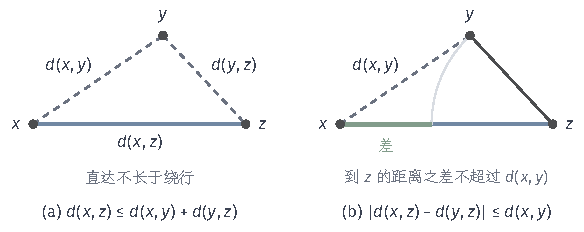
\includegraphics[width=98.972mm]{figures/02-abstract-mathematics/01-metric-and-measure/tikz/c1-triangle-inequality/figure.pdf}
  \caption{三角不等式与反向三角不等式。(a) 从$x$到$z$的直达距离（蓝色实线）不超过经中间点$y$的绕行长度（灰色虚线）。(b) 把比较点从$x$移到$y$时，到固定点$z$的两段距离之差（绿色标出的长度差）不超过移动的距离$d(x,y)$。}
  \label{fig:metric-triangle}
\end{figure}

\paragraph{集合与度量一起给出}
同一个集合可以配备不同的度量，所以度量空间是集合与度量组成的对，而不是集合本身。例如在$\mathbb R$上，除了通常距离$|x-y|$，还可以取下一小节的离散距离：任意两个不同的数距离都是$1$。在通常距离下，$1/n$与$0$的距离$1/n$越来越小；在离散距离下，这个距离始终是$1$。因此“$1/n$是否接近$0$”没有脱离度量的答案。后面凡是谈到邻近、收敛和连续，都要先说明使用的是哪个度量；在不致混淆时，才把$(X,d)$简称为$X$。

\subsection{常见度量}
\label{sec:metric-examples}

最常见的度量来自向量的范数；但度量并不要求对象能做减法，计数和路径长度同样可以给出度量。

\paragraph{由范数诱导的度量}
设$\lVert\cdot\rVert$是$\mathbb R^d$上的一个范数，即满足正定性、正齐次性$\lVert c\bm x\rVert=|c|\,\lVert\bm x\rVert$与三角不等式$\lVert\bm x+\bm y\rVert\leq\lVert\bm x\rVert+\lVert\bm y\rVert$的非负函数；常用的$\ell^1$、欧氏和最大值范数及其性质见\BookChapterRef{chap:normed-inner-product-spaces}{卷一“赋范空间与内积空间”章}。令$d(\bm x,\bm y)=\lVert\bm x-\bm y\rVert$，度量的三条要求逐条来自范数公理：正定性给出$d(\bm x,\bm y)=0\Leftrightarrow\bm x-\bm y=\bm 0$；取$c=-1$得到$\lVert\bm y-\bm x\rVert=\lVert\bm x-\bm y\rVert$，即对称性；把$\bm x-\bm z$写成$(\bm x-\bm y)+(\bm y-\bm z)$再用范数三角不等式，就得到度量的三角不等式。三种常用范数给出
\[
  \begin{aligned}
    d_1(\bm x,\bm y)&=\sum_{i=1}^d|x_i-y_i|,\qquad
    d_2(\bm x,\bm y)=\Bigl(\sum_{i=1}^d|x_i-y_i|^2\Bigr)^{1/2},\\
    d_\infty(\bm x,\bm y)&=\max_{1\leq i\leq d}|x_i-y_i|.
  \end{aligned}
\]
$d_1$把各坐标的偏差全部累加，$d_\infty$只记录最大的一个坐标偏差，$d_2$介于两者之间。

\begin{example}[同一组点的三种距离]
\label{ex:metric-three-distances}
在$\mathbb R^2$中取$\bm p=(0,0)$、$\bm q=(4,0)$、$\bm r=(3,3)$。$\bm q-\bm p=(4,0)$只有一个坐标偏差，三种距离都等于$4$。$\bm r-\bm p=(3,3)$的偏差分在两个坐标上，于是
\[
  d_1(\bm p,\bm r)=6,\qquad d_2(\bm p,\bm r)=3\sqrt2\approx4.243,\qquad d_\infty(\bm p,\bm r)=3.
\]
在$d_1$和$d_2$下$\bm q$离$\bm p$更近，在$d_\infty$下却是$\bm r$更近。图~\ref{fig:metric-three-distances}画出了三种读数：$d_1$沿坐标方向折线累加，$d_2$取直线段，$d_\infty$只看较长的那条坐标边。哪个点“更近”取决于我们怎样累计各坐标上的偏差。
\end{example}

\begin{figure}[!htbp]
  \centering
  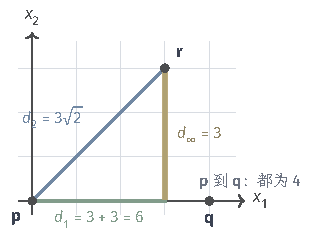
\includegraphics[width=52.871mm]{figures/02-abstract-mathematics/01-metric-and-measure/tikz/c1-three-distances/figure.pdf}
  \caption{同一组平面点在三种度量下的距离。$\bm q$与$\bm p$只在横坐标上相差$4$，三种距离都是$4$；$\bm r$与$\bm p$在两个坐标上各差$3$，$d_1$按折线累加得$6$，$d_2$取直线长度$3\sqrt2$，$d_\infty$只取较大的坐标差$3$。}
  \label{fig:metric-three-distances}
\end{figure}

\paragraph{不需要减法的度量}
在任意非空集合$X$上令$d(x,y)=0$（$x=y$）、$d(x,y)=1$（$x\neq y$），得到\term{离散度量}（discrete metric）。前两条要求直接由定义成立；对三角不等式，若$x=z$，左边为$0$；若$x\neq z$，则$y$不可能同时等于$x$和$z$，右边至少有一项为$1$。离散度量只回答“相同或不同”，不衡量差别大小，常用来构造反例。

对长度为$m$的两个二进制串$x=x_1\cdots x_m$与$y=y_1\cdots y_m$，\term{Hamming距离}（Hamming distance）定义为不同位置的个数$d_H(x,y)=\#\{i:x_i\neq y_i\}$，其中$\#$表示集合的元素个数。例如$d_H(10110,11100)=2$，两串在第2、4位不同。三角不等式逐位检查：若$x_i\neq z_i$，则$x_i\neq y_i$与$y_i\neq z_i$至少有一个成立，所以$x$与$z$不同的位置都被计入右边两项中的至少一项。这里用的是逐坐标比较，而不是对串做减法。

设$\mathcal G=(V,E)$是无权、无向的连通图，令$d_{\mathcal G}(u,v)$为从$u$到$v$的路径所含边数的最小值，即\term{最短路距离}（shortest-path distance）；最短路的计算见\BookChapterRef{chap:graph-optimization}{卷一“图上的组合优化”章}。连通性保证每对顶点之间都有路径，最小值是有限的非负整数；分离性来自“长度为零的路径只能停在原地”，对称性来自无向图中路径可以反向走。三角不等式靠路径拼接：把$u$到$w$的最短路径接上$w$到$v$的最短路径，得到一条长度为$d_{\mathcal G}(u,w)+d_{\mathcal G}(w,v)$的从$u$到$v$的通路，而最短路距离不超过任何通路的长度。若图不连通，不同连通分量的顶点之间没有路径，按惯例记为$+\infty$；这不是本章意义下取有限值的度量，此时应把讨论限制在一个连通分量上。

\subsection{子空间度量}
\label{sec:metric-subspace}

研究常常只涉及原空间的一部分对象，例如区间$[0,1]$中的实数，或单位圆周上的点。这时最自然的做法是保留原来的距离，只缩小可以取的点。

\begin{definition}[子空间度量]
\label{def:metric-subspace}
设$(X,d)$是度量空间，$A\subseteq X$非空。$d$在$A\times A$上的限制$d_A(x,y)=d(x,y)$（$x,y\in A$）称为$A$上的\term{子空间度量}（subspace metric），$(A,d_A)$称为$(X,d)$的子空间。
\end{definition}

$A$中的任意三点也是$X$中的点，所以三条要求直接从$d$继承，$d_A$确实是度量。限制之后，两点之间的距离数值不变，变化的只是可以选取的点的范围。下一节会看到，这个范围的变化足以改变“一点附近”的含义。

\paragraph{区间与圆周}
对区间$A=[0,1]\subseteq\mathbb R$，子空间距离仍是$|s-t|$，与端点是否属于$A$无关。对单位圆周$S^1=\{\bm p\in\mathbb R^2:\lVert\bm p\rVert_2=1\}$，子空间距离是欧氏距离$\lVert\bm p-\bm q\rVert_2$，也就是连接两点的弦长。若$\bm p,\bm q$所夹的圆心角为$\theta\in[0,\pi]$，弦长为$2\sin(\theta/2)$，而沿圆周行走的最短弧长是$\theta$。例如$\bm p=(1,0)$、$\bm q=(-1,0)$时，弦长为$2$，弧长为$\pi$。弧长同样满足度量的三条要求，但它是在圆周上重新规定的距离，并不是欧氏距离的限制。“限制定义域”与“重新规定距离”是两种不同的操作，得到的度量空间也不同。

\subsection{有限乘积度量}
\label{sec:metric-product}

描述一个样本可能同时需要几个分量，例如一个实数特征和一个二进制串。若每个分量所在的集合都已有度量，可以用各分量的距离组合出整体距离。

\begin{definition}[有限乘积度量]
\label{def:metric-product}
设$(X_1,d_1),\dots,(X_m,d_m)$是度量空间，$X=X_1\times\cdots\times X_m$。对$x=(x_1,\dots,x_m)$与$y=(y_1,\dots,y_m)$，令
\[
  \rho_1(x,y)=\sum_{i=1}^m d_i(x_i,y_i),\qquad
  \rho_\infty(x,y)=\max_{1\leq i\leq m}d_i(x_i,y_i).
\]
二者都称为$X$上的\term{乘积度量}（product metric）。
\end{definition}

验证只需逐坐标使用三角不等式。分离性：$\rho_1(x,y)=0$或$\rho_\infty(x,y)=0$都意味着每个$d_i(x_i,y_i)=0$，即每个坐标相同；对称性由每个$d_i$对称得到。对三角不等式，每个坐标都有$d_i(x_i,z_i)\leq d_i(x_i,y_i)+d_i(y_i,z_i)$，对$i$求和得到$\rho_1$的三角不等式；对右边分别放大为两个最大值，再对左边取最大值，得到$\rho_\infty$的三角不等式。

若各分量的单位或重要性不同，可以取固定权重$w_i>0$，令$\rho_w(x,y)=\sum_iw_id_i(x_i,y_i)$，验证方法相同。权重必须严格为正：若$w_1=0$，则只有第一坐标不同的两点距离为零，分离性失败，得到的是下一小节的伪度量。

\paragraph{两种乘积度量的比较}
对任意$x,y\in X$，和式中每一项都不超过最大项，而最大项本身是和式中的一项，所以
\begin{equation}
\label{eq:metric-product-bounds}
  \rho_\infty(x,y)\leq\rho_1(x,y)\leq m\,\rho_\infty(x,y).
\end{equation}
这组界说明，两个度量在相差常数倍的意义下给出同样的误差控制：一个趋于零当且仅当另一个趋于零。它还给出每个坐标与整体之间的关系$d_i(x_i,y_i)\leq\rho_\infty(x,y)$，后面判断逐坐标收敛、连续和完备都要用到它。常数$m$随坐标个数增长，所以这组界只适用于有限乘积；无限多个坐标的乘积需要另作设计。

\subsection{伪度量与商度量}
\label{sec:metric-pseudometric}

有些比较规则只看对象的一部分特征。例如只比较平面上两点的横坐标，令$p(\bm x,\bm y)=|x_1-y_1|$。这个规则非负、对称且满足三角不等式，但$(0,0)$与$(0,1)$的距离为零：两点不同，只是当前规则无法区分它们。

\begin{definition}[伪度量]
\label{def:metric-pseudometric}
设$X$非空。若$p:X\times X\to[0,\infty)$对任意$x,y,z\in X$满足$p(x,x)=0$、$p(x,y)=p(y,x)$与$p(x,z)\leq p(x,y)+p(y,z)$，就称$p$为$X$上的\term{伪度量}（pseudometric）。
\end{definition}

伪度量只把分离性中的“$p(x,y)=0\Rightarrow x=y$”去掉，其余要求全部保留。上面的横坐标规则就是$\mathbb R^2$上的伪度量；前一小节零权重的乘积距离也是伪度量。要从伪度量得到真正的度量，可以把相互之间距离为零的对象看成同一个新对象。

\paragraph{零距离等价类}
在伪度量空间中规定$x\sim y$当且仅当$p(x,y)=0$。这是等价关系：$p(x,x)=0$给出自反性，$p$的对称性给出对称性；若$x\sim y$且$y\sim z$，三角不等式给出$0\leq p(x,z)\leq p(x,y)+p(y,z)=0$，于是$x\sim z$，传递性成立。等价关系与商集见\BookChapterRef{chap:sets-functions-and-proofs}{卷一“集合、关系与映射”章}。记$x$所在的等价类为$[x]$，全部等价类组成的商集记为$X/{\sim}$。

\paragraph{商度量}
在商集上希望令$\bar p([x],[y])=p(x,y)$。一个等价类有许多代表元，这个数值必须先证明与代表元的选择无关。设$x\sim x'$、$y\sim y'$，三角不等式给出
\[
  p(x,y)\leq p(x,x')+p(x',y')+p(y',y)=p(x',y'),
\]
交换两组代表元的角色又得到$p(x',y')\leq p(x,y)$，所以$p(x,y)=p(x',y')$，$\bar p$是良定义的。非负性、对称性与三角不等式直接由$p$在代表元上的相应性质得到。分离性也恢复了：$\bar p([x],[y])=0$当且仅当$p(x,y)=0$，即$x\sim y$，亦即$[x]=[y]$。于是$\bar p$是$X/{\sim}$上的度量，称为\term{商度量}（quotient metric）。

\begin{example}[只比较横坐标]
\label{ex:metric-quotient-projection}
对$p(\bm x,\bm y)=|x_1-y_1|$，点$(a,b)$的等价类是竖直线$\{(a,t):t\in\mathbb R\}$。映射$[(a,b)]\mapsto a$把等价类一一对应到实数，并且$\bar p([(a,b)],[(c,e)])=|a-c|$，所以商空间就是带通常距离的实轴。图~\ref{fig:metric-pseudometric-quotient}画出了这个过程。商化并没有恢复被忽略的纵坐标，只是让新空间中的点恰好对应当前规则能够区分的对象。后面讨论函数空间时，“几乎处处相等的函数看作同一元素”也是这种构造。
\end{example}

\begin{figure}[!htbp]
  \centering
  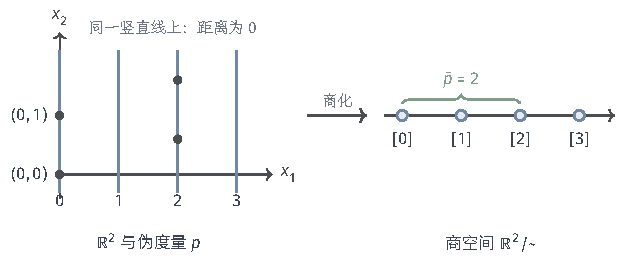
\includegraphics[width=104.916mm]{figures/02-abstract-mathematics/01-metric-and-measure/tikz/c1-pseudometric-quotient/figure.pdf}
  \caption{伪度量$p(\bm x,\bm y)=|x_1-y_1|$与商度量。左侧同一条竖直线上的点（如$(0,0)$与$(0,1)$）相互距离为零，构成一个等价类；右侧每条竖直线成为实轴上的一个点，两类之间的距离是横坐标之差，例如$|2-0|=2$。}
  \label{fig:metric-pseudometric-quotient}
\end{figure}

\section{开闭集与邻近关系}
\label{sec:metric-open-closed}

度量给出的是两点之间的数值。要谈“一点附近”“集合的边缘”“用少数点代表整个空间”，需要把这些数值组织成关于集合的判断。本节先用开球描述一点附近允许怎样移动，再由此定义开集与闭集，接着用内部、闭包与边界刻画点相对集合的位置，最后讨论能否用可数个代表点逼近空间中的每一点。本节始终固定一个度量空间$(X,d)$。

\subsection{开球与邻域}
\label{sec:metric-balls}

在实轴上，“$x$离$a$不到$r$”就是$x\in(a-r,a+r)$。一般度量空间中没有区间，但同样可以把与中心距离小于$r$的点收集起来。

\begin{definition}[开球与邻域]
\label{def:metric-open-ball}
对$a\in X$与$r>0$，集合$B(a,r)=\{x\in X:d(x,a)<r\}$称为以$a$为中心、$r$为半径的\term{开球}（open ball）。若$V\subseteq X$包含某个开球$B(a,r)$，就称$V$是$a$的一个\term{邻域}（neighborhood）。
\end{definition}

定义中的不等号是严格的，半径必须为正，因此中心本身总在球内。邻域只要求在$a$周围留出一个球的余量：实轴上的$[0,1]$是$1/2$的邻域，因为$B(1/2,1/2)=(0,1)\subseteq[0,1]$；它却不是$0$的邻域，因为每个$(-r,r)$都含有负数。

\paragraph{球的形状由度量决定}
“球”只是一个名称，它的形状完全由度量决定。在$\mathbb R^2$中，单位球$B(\bm 0,1)$在$d_2$下是圆盘内部，在$d_\infty$下是边与坐标轴平行的正方形内部$\{\bm x:|x_1|<1,|x_2|<1\}$，在$d_1$下是以四个坐标轴上的点$(\pm1,0)$、$(0,\pm1)$为顶点的菱形内部。由$\lVert\bm x\rVert_\infty\leq\lVert\bm x\rVert_2\leq\lVert\bm x\rVert_1$，三个单位球依次嵌套：$d_1$的菱形最小，$d_\infty$的正方形最大，见图~\ref{fig:metric-unit-balls}。在离散度量下，半径不超过$1$的球只含中心一个点，与“圆”毫无相似之处。

\begin{figure}[!htbp]
  \centering
  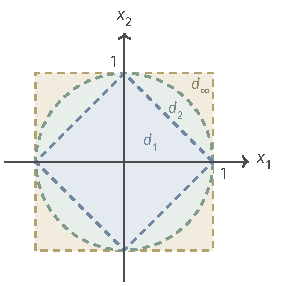
\includegraphics[width=48.055mm]{figures/02-abstract-mathematics/01-metric-and-measure/tikz/c1-unit-balls/figure.pdf}
  \caption{$\mathbb R^2$中以原点为中心的单位开球在三种度量下的形状。最内的菱形是$d_1$单位球，中间的圆盘是$d_2$单位球，最外的正方形是$d_\infty$单位球；虚线边界不属于开球。嵌套顺序对应$\lVert\bm x\rVert_\infty\leq\lVert\bm x\rVert_2\leq\lVert\bm x\rVert_1$：距离读数越大，同一半径的球越小。}
  \label{fig:metric-unit-balls}
\end{figure}

\paragraph{球内每点都有更小的球}
若$y\in B(a,r)$，令$\rho=r-d(y,a)>0$。对任意$z\in B(y,\rho)$，三角不等式给出$d(z,a)\leq d(z,y)+d(y,a)<\rho+d(y,a)=r$，所以
\begin{equation}
\label{eq:metric-ball-inside-ball}
  B(y,\rho)\subseteq B(a,r).
\end{equation}
也就是说，开球中的每一点自己也有一个留在球内的小球，这是下一小节证明“开球是开集”的依据。

\paragraph{相对开球}
设$A\subseteq X$配备子空间度量。为区分所在空间，把$A$中的开球记为$B_A(a,r)$，把$X$中的开球记为$B_X(a,r)$。对$a\in A$与$r>0$，
\begin{equation}
\label{eq:metric-relative-ball}
  B_A(a,r)=A\cap B_X(a,r),
\end{equation}
因为两边都恰好由“属于$A$且与$a$的距离小于$r$”的点组成，而子空间中的距离数值与$X$中相同。取$A=[0,1]\subseteq\mathbb R$与端点$0$，当$0<r\leq1$时，$B_A(0,r)=[0,1]\cap(-r,r)=[0,r)$。于是$[0,1/2)$在$A$中是$0$的邻域，在$\mathbb R$中却不是。图~\ref{fig:metric-relative-ball}画出了这个交集。判断邻域时，必须先说明当前所在的空间。

\begin{figure}[!htbp]
  \centering
  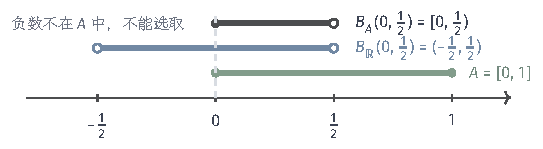
\includegraphics[width=91.934mm]{figures/02-abstract-mathematics/01-metric-and-measure/tikz/c1-relative-ball/figure.pdf}
  \caption{子空间中的相对开球。环境空间$\mathbb R$中的球$B_{\mathbb R}(0,r)=(-r,r)$（蓝色）伸到负半轴，而负数不属于子空间$A=[0,1]$（绿色）；二者的交集就是$A$中的球$B_A(0,r)=[0,r)$，它包含端点$0$。图中取$r=1/2$。}
  \label{fig:metric-relative-ball}
\end{figure}

\subsection{开集与闭集}
\label{sec:metric-open-sets}

邻域描述的是单个点。若一个集合是其中每一点的邻域，集合中的点无论在哪里，都可以向各个方向稍作移动而不离开它。

\begin{definition}[开集与闭集]
\label{def:metric-open-closed}
若对每个$x\in U$都存在$r>0$使$B(x,r)\subseteq U$，就称$U\subseteq X$为\term{开集}（open set）。若$X\setminus F$是开集，就称$F\subseteq X$为\term{闭集}（closed set）。
\end{definition}

半径可以随点改变，越靠近边缘的点可用的球越小。由式~\eqref{eq:metric-ball-inside-ball}，每个开球都是开集。空集没有需要检查的点，所以是开集；$X$包含它的每个球，所以也是开集。二者互为补集，因此它们同时也是闭集。

\begin{theorem}[开集与闭集的运算]
\label{thm:metric-open-operations}
任意多个开集的并是开集，有限多个开集的交是开集；任意多个闭集的交是闭集，有限多个闭集的并是闭集。
\end{theorem}

\begin{proof}
设$\{U_\alpha\}$是一族开集，$x\in\bigcup_\alpha U_\alpha$。则$x$属于某个$U_\beta$，存在$r>0$使$B(x,r)\subseteq U_\beta\subseteq\bigcup_\alpha U_\alpha$，所以并集是开集。

设$U_1,\dots,U_k$是开集，$x\in\bigcap_{i=1}^kU_i$。对每个$i$取$r_i>0$使$B(x,r_i)\subseteq U_i$，令$r=\min_ir_i$。由于只有有限个正数，$r>0$，而且$B(x,r)\subseteq B(x,r_i)\subseteq U_i$对每个$i$成立，所以$B(x,r)\subseteq\bigcap_iU_i$。

闭集的两条结论由补集关系得到：$X\setminus\bigcap_\alpha F_\alpha=\bigcup_\alpha(X\setminus F_\alpha)$是开集的并，$X\setminus\bigcup_{i=1}^kF_i=\bigcap_{i=1}^k(X\setminus F_i)$是有限个开集的交。
\end{proof}

证明中“有限”的作用在于取最小值时得到正数；对无限多个半径，下确界可能是零。例如每个$(-1/n,1/n)$都是$\mathbb R$中的开集，它们的交却是$\{0\}$，不是开集，因为$0$的每个球都含有非零数。同理，每个$[1/n,1]$都是闭集，它们的并$(0,1]$却不是闭集：补集$(-\infty,0]\cup(1,\infty)$在点$0$处没有留在其中的球。

\paragraph{开与闭不是互斥的两类}
“不开”不意味着“闭”。$X$与$\varnothing$既开又闭；实轴上的$[0,1)$既不开也不闭：$0\in[0,1)$没有留在其中的球，所以它不是开集；$1$在补集中，但每个$B(1,r)$都含有$[0,1)$中的点，所以补集不是开集。

\paragraph{子空间中的开集与闭集}
开与闭还取决于所在空间。由式~\eqref{eq:metric-relative-ball}可以把子空间中的开集化为环境空间的开集。

\begin{lemma}[子空间的开集与闭集]
\label{lem:metric-relative-open}
设$A\subseteq X$配备子空间度量。$U\subseteq A$是$A$中的开集，当且仅当存在$X$中的开集$V$使$U=A\cap V$；$F\subseteq A$是$A$中的闭集，当且仅当存在$X$中的闭集$C$使$F=A\cap C$。
\end{lemma}

\begin{proof}
若$U=A\cap V$且$V$在$X$中开，对$x\in U$取$r>0$使$B_X(x,r)\subseteq V$，则$B_A(x,r)=A\cap B_X(x,r)\subseteq A\cap V=U$，所以$U$在$A$中开。反过来，若$U$在$A$中开，对每个$x\in U$取$r_x>0$使$B_A(x,r_x)\subseteq U$，令$V=\bigcup_{x\in U}B_X(x,r_x)$。$V$是开球的并，在$X$中开；并且$A\cap V=\bigcup_{x\in U}B_A(x,r_x)$，它包含每个$x\in U$，又包含于$U$，所以等于$U$。

对闭集，$F$在$A$中闭当且仅当$A\setminus F$在$A$中开，即$A\setminus F=A\cap V$对某个$X$中的开集$V$成立；这又等价于$F=A\cap(X\setminus V)$，其中$X\setminus V$在$X$中闭。
\end{proof}

例如在子空间$A=[0,1]$中，$[0,1/2)=A\cap(-1,1/2)$与$(1/2,1]=A\cap(1/2,2)$都是开集，尽管它们在$\mathbb R$中都不是开集；$[0,1/2]=A\cap[-1,1/2]$是$A$中的闭集。$A$本身在$A$中既开又闭，这与它在$\mathbb R$中只闭不开并不矛盾。

\subsection{内部、闭包与边界}
\label{sec:metric-closure}

同一族开球还可以对单个点相对集合的位置分类：点可能深入集合内部，可能紧贴集合，也可能同时贴着集合与它的补集。

\begin{definition}[内部、闭包与边界]
\label{def:metric-closure}
设$A\subseteq X$。若存在$r>0$使$B(x,r)\subseteq A$，称$x$为$A$的内点，全部内点组成$A$的\term{内部}（interior），记作$A^\circ$。若对每个$r>0$都有$B(x,r)\cap A\neq\varnothing$，称$x$为$A$的闭包点，全部闭包点组成$A$的\term{闭包}（closure），记作$\overline A$。若对每个$r>0$，$B(x,r)$既与$A$相交又与$X\setminus A$相交，称$x$为$A$的边界点，全部边界点组成$A$的\term{边界}（boundary），记作$\partial A$。
\end{definition}

三个定义的区别在量词：内点要求“存在一个球”留在集合内，闭包点要求“每个球”都碰到集合，边界点要求“每个球”同时碰到两侧。按定义$A^\circ\subseteq A\subseteq\overline A$，因为$x\in A$时每个球都含有$x$本身。图~\ref{fig:metric-interior-closure-boundary}画出了三类位置。

\begin{figure}[!htbp]
  \centering
  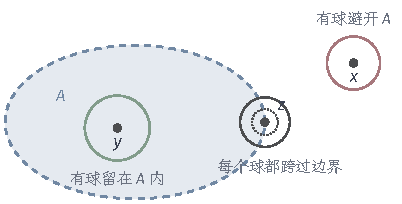
\includegraphics[width=68.104mm]{figures/02-abstract-mathematics/01-metric-and-measure/tikz/c1-interior-closure-boundary/figure.pdf}
  \caption{点相对集合$A$（浅蓝区域，虚线边界不属于$A$）的三种位置。内点$y$有一个完全落在$A$中的球；边界点$z$的每个球都同时碰到$A$与补集，它在$\overline A$中却可以不属于$A$；点$x$有一个完全避开$A$的球，所以$x\notin\overline A$。}
  \label{fig:metric-interior-closure-boundary}
\end{figure}

\paragraph{边界等于闭包去掉内部}
$x\notin A^\circ$恰好表示没有球留在$A$中，即每个球都碰到$X\setminus A$。所以边界点就是“既是闭包点、又不是内点”的点：
\begin{equation}
\label{eq:metric-boundary}
  \partial A=\overline A\setminus A^\circ.
\end{equation}
在$\mathbb R$中，$(0,1)$与$[0,1]$的内部都是$(0,1)$，闭包都是$[0,1]$，边界都是$\{0,1\}$：边界点可以属于集合，也可以不属于集合。有理数集$\mathbb Q$的情形更极端：每个区间都同时含有有理数和无理数，所以$\mathbb Q^\circ=\varnothing$、$\overline{\mathbb Q}=\mathbb R$、$\partial\mathbb Q=\mathbb R$。

\paragraph{闭包是闭集}
若$x\notin\overline A$，存在$r>0$使$B(x,r)\cap A=\varnothing$。对$y\in B(x,r)$，取$\rho=r-d(x,y)$，由式~\eqref{eq:metric-ball-inside-ball}，$B(y,\rho)\subseteq B(x,r)$也避开$A$，所以$y\notin\overline A$。于是$X\setminus\overline A$包含其每一点的一个球，是开集。由此得到：$A$是闭集当且仅当$A=\overline A$。若$A$闭而$x\notin A$，则$x$属于开集$X\setminus A$，有一个避开$A$的球，$x\notin\overline A$，故$\overline A\subseteq A$；反过来，$A=\overline A$时$A$就是闭集。对内部有对称的结论：$A^\circ$是开集，$A$开当且仅当$A=A^\circ$；论证只需把“避开$A$”换成“留在$A$内”。

\paragraph{点到集合的距离}
“每个球都碰到$A$”还可以写成一个数值条件。对非空集合$A$，定义点$x$到$A$的距离
\begin{equation}
\label{eq:metric-distance-to-set}
  d(x,A)=\inf_{a\in A}d(x,a).
\end{equation}
它是有限的非负数，因为任取$a_0\in A$都有$0\leq d(x,A)\leq d(x,a_0)$。由下确界的定义，对任意$\varepsilon>0$都有$a\in A$使$d(x,a)<d(x,A)+\varepsilon$。

\begin{lemma}[距离为零与闭包]
\label{lem:metric-distance-closure}
设$A\subseteq X$非空。则$x\in\overline A$当且仅当$d(x,A)=0$。
\end{lemma}

\begin{proof}
若$d(x,A)=0$，对每个$r>0$，由下确界的逼近性质有$a\in A$使$d(x,a)<r$，即$B(x,r)\cap A\neq\varnothing$，所以$x\in\overline A$。反过来，若$x\in\overline A$，对每个$r>0$有$a\in B(x,r)\cap A$，于是$d(x,A)\leq d(x,a)<r$；$r$任意，故$d(x,A)=0$。
\end{proof}

距离为零只说明$x$紧贴$A$，并不说明$x\in A$：$d(0,(0,1))=0$，而$0\notin(0,1)$。下确界也不一定由$A$中的某个“最近点”达到：$d(2,(0,1))=1$，但对每个$a\in(0,1)$都有$|2-a|>1$。什么条件能保证最近点存在，要等到第~\ref{sec:metric-continuous-maps}节讨论紧致集上的连续函数时回答。

\subsection{稠密集与可分空间}
\label{sec:metric-separable}

计算中只能存储有理数，却可以把任何实数逼近到任意精度。这说明一个较小的集合可以“代表”整个空间：它不必包含每一点，但必须与每一点任意接近。

\begin{definition}[稠密集与可分空间]
\label{def:metric-separable}
若$\overline D=X$，就称$D\subseteq X$在$X$中\term{稠密}（dense）。若$X$存在可数的稠密子集，就称$X$是\term{可分}（separable）的。
\end{definition}

按闭包的定义，$D$稠密等价于每个开球$B(x,r)$都与$D$相交：无论指定哪个位置$x$和哪个精度$r$，$D$中总有一点在该精度内代表$x$。可分性的要求更强，它要求同一套可数个代表点服务所有位置和所有精度。可数集合的概念见\BookChapterRef{chap:cardinality}{卷一“基数”章}。

\paragraph{实轴与离散空间}
在通常距离下，任意区间$(x-r,x+r)$都含有有理数，所以$\mathbb Q$在$\mathbb R$中稠密，而$\mathbb Q$可数，$\mathbb R$是可分的；同理，$\mathbb Q^d$在$(\mathbb R^d,d_2)$中稠密，因为对每个坐标取误差小于$r/\sqrt d$的有理数，所得点的欧氏误差小于$r$。另一方面，在不可数集合（例如$\mathbb R$本身）上取离散度量，每个单点集都是开球$B(x,1/2)=\{x\}$，稠密集必须与每个单点相交，只能是全空间，因而不可数，空间不可分。两个例子使用同一个底集$\mathbb R$，只因度量不同，可分性就不同。可分也不意味着空间本身可数：$\mathbb R$不可数，却有可数稠密子集$\mathbb Q$。

图~\ref{fig:metric-unit-balls}中的球形状和本节的相对球已经表明，邻近结构由度量和所在空间共同决定。下一节用这套邻近结构研究点列：给定精度后，点列的项最终能否都落进某个球内。

\section{点列收敛与完备性}
\label{sec:metric-convergence-completeness}

实数列$a_n\to a$的含义是误差$|a_n-a|$趋于零。把绝对值换成一般距离，就得到度量空间中的收敛。但这只回答了一类问题：已经有一个候选极限，检查点列是否逼近它。迭代求解、逐次逼近等问题往往事先不知道极限在哪里，只能观察点列内部的项是否越来越接近。本节先建立收敛和它与闭集的关系，再研究后一类问题，并说明怎样把缺失的极限补进空间。

\subsection{点列的收敛}
\label{sec:metric-convergence}

\begin{definition}[点列的收敛]
\label{def:metric-convergence}
设$(x_n)$是$X$中的点列，$x\in X$。若$d(x_n,x)\to0$，即对任意$\varepsilon>0$存在$N$使$n\geq N$时$d(x_n,x)<\varepsilon$，就称$(x_n)$\term{收敛}（converge）到$x$，记作$x_n\to x$，称$x$为它的极限。
\end{definition}

用开球的语言说，$x_n\to x$表示无论球$B(x,\varepsilon)$多小，点列从某项起都留在球中。实数列的情形见\BookChapterRef{chap:limits-continuity}{卷一“极限与连续”章}，那里的误差$|a_n-a|$在这里换成了$d(x_n,x)$。定义要求极限$x$属于当前空间$X$；如果所谓的极限在$X$之外，那么在$X$中这一列不收敛。

\paragraph{极限的基本性质}
三条基本性质都由三角不等式得到，区别在于各自控制的量。第一，极限唯一：若$x_n\to x$且$x_n\to y$，则$0\leq d(x,y)\leq d(x,x_n)+d(x_n,y)\to0$，故$d(x,y)=0$，$x=y$。第二，收敛列有界：取$\varepsilon=1$得到$N$，则对任意$n$，$d(x_n,x)\leq\max\{1,d(x_1,x),\dots,d(x_{N-1},x)\}$，所有项都落在以$x$为中心的一个有限半径球内。第三，子列保持原极限：若$n_1<n_2<\cdots$，则$n_k\geq k$，所以$k\geq N$时$d(x_{n_k},x)<\varepsilon$。

\paragraph{有限乘积中的收敛}
在有限乘积$X=X_1\times\cdots\times X_m$上取乘积度量$\rho_\infty$或$\rho_1$。由式~\eqref{eq:metric-product-bounds}，$d_i(x_{n,i},x_i)\leq\rho_\infty(x_n,x)\leq\rho_1(x_n,x)\leq\sum_{i=1}^md_i(x_{n,i},x_i)$，其中$x_{n,i}$表示$x_n$的第$i$个坐标。左边的不等式说明整体收敛推出每个坐标收敛；右边的不等式说明各坐标收敛时，有限个趋于零的数之和也趋于零，从而整体收敛。所以在有限乘积中，整体收敛与逐坐标收敛等价，且与选$\rho_1$还是$\rho_\infty$无关。$\mathbb R^d$上$d_1$与$d_\infty$下的收敛都等价于逐坐标收敛；由$d_\infty\leq d_2\leq d_1$，$d_2$下的收敛也是如此。

\paragraph{极限可能不在当前空间中}
取子空间$X=(0,1)$与点列$x_n=1/(n+1)$。在环境空间$\mathbb R$中，$x_n\to0$；但$0\notin X$，而极限唯一，所以$(x_n)$在$X$中没有极限。点列本身没有改变，改变的是允许作为极限的点。

\subsection{闭包与闭集的序列判据}
\label{sec:metric-sequential-closure}

闭包用“每个球都碰到集合”定义，这是关于所有半径的条件。点列把这些半径排成一列$1/n$，于是闭包点可以用集合内的点逐项逼近。

\begin{lemma}[闭包的序列判据]
\label{lem:metric-sequential-closure}
设$A\subseteq X$。则$x\in\overline A$当且仅当存在$A$中的点列$(a_n)$使$a_n\to x$。
\end{lemma}

\begin{proof}
设$x\in\overline A$。对每个$n$，球$B(x,1/n)$与$A$相交，从中取一点$a_n$，则$d(a_n,x)<1/n\to0$。反过来，设$a_n\in A$且$a_n\to x$。对任意$r>0$，存在$n$使$d(a_n,x)<r$，即$a_n\in B(x,r)\cap A$，所以每个球都与$A$相交，$x\in\overline A$。
\end{proof}

由第~\ref{sec:metric-closure}小节，$A$闭当且仅当$\overline A\subseteq A$。结合引理~\ref{lem:metric-sequential-closure}，得到闭集的序列判据：$A$是闭集，当且仅当$A$中的点列只要在$X$中收敛，其极限就属于$A$。例如$[0,1]$在$\mathbb R$中闭，而$(0,1]$不闭，因为$1/n\in(0,1]$收敛到$0\notin(0,1]$。

这个判据只承诺保留已经存在的极限，并不保证点列有极限。$\mathbb Q$在$\mathbb Q$自身中是闭集（全空间总是闭的），但下面会看到，$\mathbb Q$中有项彼此越来越近却没有极限的点列。要讨论极限的存在，需要一个不预先指定候选极限的判据。

\subsection{柯西列与完备性}
\label{sec:metric-cauchy}

用逐次逼近求解时，我们只能看到已经算出的项。若从某项起任意两项都足够接近，就有理由期望点列趋于某个极限；但这需要空间里确实有那个极限。

\begin{definition}[柯西列与完备空间]
\label{def:metric-complete}
若对任意$\varepsilon>0$存在$N$，使$m,n\geq N$时$d(x_m,x_n)<\varepsilon$，就称$(x_n)$为\term{柯西列}（Cauchy sequence）。若$X$中的每个柯西列都收敛到$X$中的某点，就称$(X,d)$是\term{完备}（complete）的，也称完备度量空间。
\end{definition}

柯西条件只涉及点列自身的项，不涉及任何候选极限。收敛列一定是柯西列：若$x_n\to x$，对$\varepsilon>0$取$N$使$n\geq N$时$d(x_n,x)<\varepsilon/2$，则$m,n\geq N$时$d(x_m,x_n)\leq d(x_m,x)+d(x,x_n)<\varepsilon$。反过来不一定成立，结论取决于空间。

\begin{example}[有理数中不收敛的柯西列]
\label{ex:metric-rational-cauchy}
令$q_n$为$\sqrt2$的十进制展开截到小数点后第$n$位，即$q_0=1$、$q_1=1.4$、$q_2=1.41$、$q_3=1.414$、$q_4=1.4142$，以此类推。每个$q_n$都是有理数，并且$q_n\leq\sqrt2<q_n+10^{-n}$。当$m\geq n$时，$q_m$与$q_n$的前$n$位相同，所以$0\leq q_m-q_n<10^{-n}$，$(q_n)$是$\mathbb Q$中（通常距离下）的柯西列。在$\mathbb R$中$q_n\to\sqrt2$，而$\sqrt2$是无理数；由极限唯一性，$(q_n)$在$\mathbb Q$中没有极限。所以$\mathbb Q$不完备。图~\ref{fig:metric-rational-cauchy}画出了这些项向$\sqrt2$处的“空缺”聚拢的情形。
\end{example}

\begin{figure}[!htbp]
  \centering
  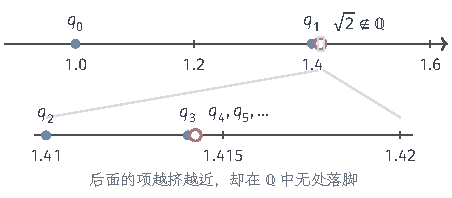
\includegraphics[width=76.616mm]{figures/02-abstract-mathematics/01-metric-and-measure/tikz/c1-rational-cauchy/figure.pdf}
  \caption{有理数中不收敛的柯西列。上方数轴上的蓝点是$\sqrt2$的十进制截断$1,\ 1.4,\ 1.41,\ 1.414$，空心圆标出$\sqrt2\approx1.41421$，它不属于$\mathbb Q$；下方放大$[1.41,1.42]$一段，可见后面的项继续向空心圆聚拢。从第$n$项起任意两项相差不到$10^{-n}$，但在$\mathbb Q$中找不到它们的极限。}
  \label{fig:metric-rational-cauchy}
\end{figure}

\paragraph{实数与欧氏空间的完备性}
实数在通常距离下是完备的，这正是卷一“极限与连续”章中的柯西收敛准则，它依赖实数的确界性质。由此可以得到$\mathbb R^d$的完备性：若$(\bm x_n)$在$d_2$下是柯西列，由$|x_{m,i}-x_{n,i}|\leq d_2(\bm x_m,\bm x_n)$，每个坐标都是实数柯西列，各自收敛到某个$x_i$；令$\bm x=(x_1,\dots,x_d)$，由上一小节，逐坐标收敛推出$d_2(\bm x_n,\bm x)\to0$。同样的论证适用于$d_1$与$d_\infty$。

\paragraph{完备子集与闭子集}
完备性与闭性之间有两个方向不同的结论，前者需要环境空间完备，后者对任意度量空间成立。

\begin{theorem}[完备性与闭集]
\label{thm:metric-complete-closed}
设$A\subseteq X$配备子空间度量。
\begin{enumerate}
  \item 若$X$完备且$A$在$X$中闭，则$A$完备。
  \item 若$A$完备，则$A$在$X$中闭。
\end{enumerate}
\end{theorem}

\begin{proof}
(1) 设$(a_n)$是$A$中的柯西列。子空间距离与$X$中的距离相同，所以它也是$X$中的柯西列，由$X$完备，存在$x\in X$使$a_n\to x$。$A$闭，由闭集的序列判据，$x\in A$，所以$(a_n)$在$A$中收敛。

(2) 设$a_n\in A$且在$X$中$a_n\to x$。收敛列是柯西列，所以$(a_n)$是$A$中的柯西列；$A$完备，存在$a\in A$使$a_n\to a$。在$X$中极限唯一，故$x=a\in A$。由闭集的序列判据，$A$闭。
\end{proof}

于是$[0,1]$在通常距离下完备，而$(0,1)$不完备：后者在$\mathbb R$中不闭，由结论(2)不可能完备。结论(1)中的完备性假设不能省去：$\mathbb Q$在$\mathbb Q$中闭，却不完备。

\paragraph{有限乘积的完备性}
设$(X_i,d_i)$都完备，$X=X_1\times\cdots\times X_m$取$\rho_\infty$。若$(x_n)$是$X$中的柯西列，由$d_i(x_{m,i},x_{n,i})\leq\rho_\infty(x_m,x_n)$，每个坐标列都是$X_i$中的柯西列，收敛到某个$x_i\in X_i$；再由逐坐标收敛等价于整体收敛，$x_n\to(x_1,\dots,x_m)$。所以有限个完备空间的乘积仍完备，对$\rho_1$亦然。上一段$\mathbb R^d$的完备性是它的特例。

\subsection{度量空间的完备化}
\label{sec:metric-completion}

$\mathbb Q$的柯西列“想要”收敛到的点，正是实数。能否对一般度量空间做同样的事：用柯西列代表缺失的极限，构造一个完备空间，使原空间稠密地放在其中，且原有距离不变？答案是肯定的，构造恰好用到第~\ref{sec:metric-pseudometric}小节的商度量。

\paragraph{用柯西列代表新点}
设$\mathcal C$是$X$中全部柯西列组成的集合。对$(x_n),(y_n)\in\mathcal C$，由反向三角不等式~\eqref{eq:metric-reverse-triangle}使用两次，
\[
  \begin{aligned}
    \bigl|d(x_m,y_m)-d(x_n,y_n)\bigr|
    &\leq\bigl|d(x_m,y_m)-d(x_n,y_m)\bigr|\\
    &\quad+\bigl|d(x_n,y_m)-d(x_n,y_n)\bigr|\\
    &\leq d(x_m,x_n)+d(y_m,y_n).
  \end{aligned}
\]
右边在$m,n\to\infty$时趋于零，所以$\bigl(d(x_n,y_n)\bigr)$是实数柯西列。由实数的完备性，极限
\[
  D\bigl((x_n),(y_n)\bigr)=\lim_{n\to\infty}d(x_n,y_n)
\]
存在。$D$非负、对称，并且对三列逐项写出$d(x_n,z_n)\leq d(x_n,y_n)+d(y_n,z_n)$后取极限，得到三角不等式。但两列不同的柯西列可能有$D=0$，例如$(1/n)$与$(-1/n)$，所以$D$只是$\mathcal C$上的伪度量。按第~\ref{sec:metric-pseudometric}小节，把$D=0$的柯西列识别为同一点，得到商集$\widehat X=\mathcal C/{\sim}$及其上的度量$\hat d$。两列的距离趋于零，意味着它们“想要趋于同一点”，识别它们正符合这一直观。

\paragraph{原空间的等距嵌入}
对$x\in X$，常值列$(x,x,\dots)$是柯西列，令$\iota(x)$为它的等价类。则$\hat d(\iota(x),\iota(y))=\lim_nd(x,y)=d(x,y)$，所以$\iota$保持距离，原空间连同它的度量被原样放进$\widehat X$。$\iota(X)$在$\widehat X$中稠密：设$\xi\in\widehat X$由柯西列$(x_n)$代表，对$\varepsilon>0$取$N$使$m,n\geq N$时$d(x_m,x_n)<\varepsilon$，则对$m\geq N$，$\hat d(\iota(x_m),\xi)=\lim_nd(x_m,x_n)\leq\varepsilon$。

\begin{theorem}[完备化]
\label{thm:metric-completion}
$(\widehat X,\hat d)$是完备度量空间，$\iota:X\to\widehat X$保持距离，且$\iota(X)$在$\widehat X$中稠密。称$\widehat X$为$X$的\term{完备化}（completion）。
\end{theorem}

\begin{proof}
度量性与嵌入的两条性质已在上面证明，只剩完备性。设$(\xi_k)$是$\widehat X$中的柯西列。由稠密性，对每个$k$取$x_k\in X$使$\hat d(\iota(x_k),\xi_k)<1/k$。因为$\iota$保持距离，
\[
  d(x_k,x_l)=\hat d(\iota(x_k),\iota(x_l))<\frac1k+\hat d(\xi_k,\xi_l)+\frac1l,
\]
右边在$k,l\to\infty$时趋于零，所以$(x_k)$是$X$中的柯西列，它代表$\widehat X$中的一点$\xi$。最后，
\[
  \hat d(\xi_k,\xi)\leq\hat d(\xi_k,\iota(x_k))+\hat d(\iota(x_k),\xi)<\frac1k+\lim_{l\to\infty}d(x_k,x_l).
\]
对$\varepsilon>0$，当$k$充分大时，$1/k<\varepsilon$，且对一切充分大的$l$有$d(x_k,x_l)<\varepsilon$，所以右边小于$2\varepsilon$。因此$\xi_k\to\xi$。
\end{proof}

这一构造的要点是：保留原来的距离，并稠密地补入全部缺失的极限。对$X=\mathbb Q$，把有理柯西列$(q_n)$所代表的点对应到它在$\mathbb R$中的极限：$D=0$的两列有相同的实数极限，所以这个对应良定义；$|\lim q_n-\lim r_n|=\lim|q_n-r_n|$说明它保持距离；每个实数都是其十进制截断的极限，所以它是满射。于是$\widehat{\mathbb Q}$与$\mathbb R$之间有保持距离的双射。对已经完备的$X$，每个柯西列都已有极限，$\iota$是满射，完备化不增加新点。完备化在保持距离的意义下唯一，证明需要把等距映射从稠密子集延拓到整个空间，这里不展开。

\section{紧致性}
\label{sec:metric-compactness}

实轴上的闭区间有两条重要性质：其中的数列总有收敛子列，连续函数在其上取得最大值和最小值。开区间$(0,1)$和整条实轴都没有这些性质。本节寻找一般度量空间中与“闭区间”对应的条件。它的核心是有限性：无论精度多高，集合都能由有限个小球控制。我们先从覆盖的角度提出这一要求，再把它与收敛子列、完备性联系起来。

\subsection{有界集与全有界集}
\label{sec:metric-totally-bounded}

“集合不太大”最直接的说法是：它能装进一个有限半径的球中。

\begin{definition}[有界集]
\label{def:metric-bounded}
若存在$a\in X$与$R<\infty$使$A\subseteq B(a,R)$，就称$A\subseteq X$是\term{有界}（bounded）的。非空集合$A$的\term{直径}（diameter）定义为$\operatorname{diam}A=\sup_{x,y\in A}d(x,y)$。
\end{definition}

两种说法等价：若$A\subseteq B(a,R)$，三角不等式给出$d(x,y)\leq d(x,a)+d(a,y)<2R$，所以$\operatorname{diam}A\leq2R$；反过来，若$\operatorname{diam}A<\infty$，任取$a\in A$，则$A\subseteq B(a,\operatorname{diam}A+1)$。

有界只控制集合的总体范围，不控制集合的内部能否在细尺度下被少量信息描述。离散度量下的无限集合$X$直径为$1$，因而有界；但用半径$1/2$的球覆盖它时，每个球只含一个点，需要无限多个球。下面的定义要求每个尺度都只需有限个球。

\begin{definition}[全有界与$\varepsilon$网]
\label{def:metric-totally-bounded}
设$A\subseteq X$，$\varepsilon>0$。若有限集$\{a_1,\dots,a_k\}\subseteq A$满足$A\subseteq\bigcup_{i=1}^kB(a_i,\varepsilon)$，就称它是$A$的一个有限$\varepsilon$网（finite $\varepsilon$-net），不指明精度时简称\term{有限网}。若对每个$\varepsilon>0$，$A$都有有限$\varepsilon$网，就称$A$是\term{全有界}（totally bounded）的。
\end{definition}

$\varepsilon$网中的点是在精度$\varepsilon$下代表$A$的有限个样本：$A$中每一点都与某个代表点相距不到$\varepsilon$。代表点的个数和位置可以随$\varepsilon$改变，精度越高通常需要越多代表点，但对每个精度都必须是有限个。图~\ref{fig:metric-epsilon-net}画出了同一个集合在两种精度下的网。

\begin{figure}[!htbp]
  \centering
  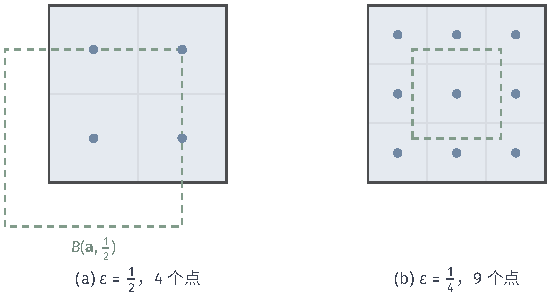
\includegraphics[width=93.169mm]{figures/02-abstract-mathematics/01-metric-and-measure/tikz/c1-epsilon-net/figure.pdf}
  \caption{正方形$[0,1]^2$在$d_\infty$下的有限$\varepsilon$网。把正方形等分为小格，蓝点取在各小格中心，小格中的点与该格中心的$d_\infty$距离至多为半个格宽。(a) $\varepsilon=1/2$时用$4$个点$\bigl((2i-1)/4,(2j-1)/4\bigr)$，格内距离至多$1/4<1/2$；虚线正方形是其中一个球$B(\bm a,1/2)$。(b) $\varepsilon=1/4$时用$9$个点$\bigl((2i-1)/6,(2j-1)/6\bigr)$，格内距离至多$1/6<1/4$。精度提高时代表点增多，但始终是有限个。}
  \label{fig:metric-epsilon-net}
\end{figure}

\paragraph{全有界推出有界与可分}
全有界比有界强。取一个有限$1$网$\{a_1,\dots,a_k\}$，任意$x,y\in A$分别落在某个$B(a_i,1)$与$B(a_j,1)$中，于是$d(x,y)<2+\max_{i,j}d(a_i,a_j)$，$A$有界。全有界还推出$A$（作为子空间）可分：对每个$n$取一个有限$1/n$网$F_n$，令$D=\bigcup_nF_n$，它是可数个有限集的并，因而可数。对任意$x\in A$与$r>0$，取$n>1/r$，$F_n$中有一点与$x$相距小于$1/n<r$，所以$D$在$A$中稠密。

\paragraph{三个要求的区别}
两个反例说明这些蕴含不能反过来。无限离散空间有界，但对$\varepsilon=1/2$没有有限网，因而不全有界。通常距离下的$\mathbb R$可分（有可数稠密集$\mathbb Q$），却无界，也就不全有界。有界控制总体范围，可分要求一套可数代表服务于所有精度，全有界则要求每个精度下只需有限个代表；三者各自约束不同的东西。

\subsection{开覆盖与紧致集}
\label{sec:metric-open-cover}

全有界允许我们为每个精度挑选最方便的一组球。有些论证中，球不是我们挑的，而是别人给定的一族开集，例如“每一点各自有一个让函数变化不大的邻域”。紧致性要求：无论给定怎样的开覆盖，都能从中选出有限个成员完成覆盖。

\begin{definition}[紧致集]
\label{def:metric-compact}
若一族开集$\{U_\alpha\}_{\alpha\in I}$满足$X=\bigcup_{\alpha\in I}U_\alpha$，就称它是$X$的一个\term{开覆盖}（open cover）。若$X$的每个开覆盖都有有限子族$U_{\alpha_1},\dots,U_{\alpha_k}$仍覆盖$X$，就称度量空间$X$是\term{紧致}（compact）的。若子集$K\subseteq X$配备子空间度量后是紧致的，就称$K$是紧致集（或紧集）。
\end{definition}

由引理~\ref{lem:metric-relative-open}，$K$中的开集都形如$K\cap V$，$V$在$X$中开。所以$K$紧致，等价于：每一族满足$K\subseteq\bigcup_\alpha V_\alpha$的$X$中的开集都有有限子族仍覆盖$K$。定义中的“有限子覆盖”必须从给定的覆盖中挑选，不能另换一组更方便的开集；正是这一点使紧致性比全有界强。

\paragraph{紧致集全有界且闭}
把全部半径为$\varepsilon$的球$\{B_K(x,\varepsilon):x\in K\}$作为开覆盖代入定义，有限子覆盖的中心就是一个有限$\varepsilon$网，所以紧致集全有界。紧致集还在任何环境空间中都是闭集。设$x\in X\setminus K$。对每个$y\in K$，令$r_y=d(x,y)/2>0$，开球$B(y,r_y)$覆盖$K$，取有限子覆盖$B(y_1,r_{y_1}),\dots,B(y_k,r_{y_k})$，令$r=\min_ir_{y_i}>0$。若$z\in B(x,r)\cap B(y_i,r_{y_i})$，则$d(x,y_i)\leq d(x,z)+d(z,y_i)<r+r_{y_i}\leq2r_{y_i}=d(x,y_i)$，矛盾；所以$B(x,r)$与$K$不交。外点都有避开$K$的球，$K$闭。

\begin{example}[全有界而不紧致]
\label{ex:metric-open-interval-cover}
$(0,1)$在通常距离下全有界：对$\varepsilon>0$，取有限个间距小于$\varepsilon$的点即可。但$(0,1)$不紧致。令$U_n=(1/n,1)$（$n\geq2$），每一点$x\in(0,1)$在$n>1/x$时属于$U_n$，所以$\{U_n\}$覆盖$(0,1)$。任取有限个$U_{n_1},\dots,U_{n_k}$，它们的并是$(1/N,1)$，其中$N=\max_in_i$，它漏掉了$(0,1/N]$中的点。图~\ref{fig:metric-open-cover-interval}画出了这个覆盖。用有限个小球覆盖$(0,1)$并不困难，难点在于这个给定覆盖的成员越来越靠近$0$而永远不包含它附近的全部点。
\end{example}

\begin{figure}[!htbp]
  \centering
  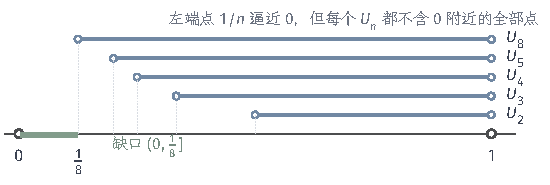
\includegraphics[width=93.105mm]{figures/02-abstract-mathematics/01-metric-and-measure/tikz/c1-open-cover/figure.pdf}
  \caption{开区间$(0,1)$的一个没有有限子覆盖的开覆盖。各条蓝色线段是$U_n=(1/n,1)$，$n=2,3,4,5,8$，它们的左端点$1/n$逐渐逼近$0$却不到达$0$；任取有限个成员，并集是某个$(1/N,1)$，在$0$附近留下绿色标出的缺口$(0,1/N]$。}
  \label{fig:metric-open-cover-interval}
\end{figure}

无限离散空间提供了另一类反例：它闭（作为全空间）且有界，但全部单点开球$\{\{x\}\}$组成开覆盖，任何有限子族只覆盖有限个点，所以不紧致。在一般度量空间中，“闭且有界”不足以推出紧致。

\subsection{紧致性的序列刻画}
\label{sec:metric-sequential-compactness}

闭区间上“数列有收敛子列”的性质也可以作为紧致性的定义。在度量空间中，它与开覆盖的定义等价。

\begin{definition}[序列紧致]
\label{def:metric-sequentially-compact}
若$K$中的每个点列都有在$K$中收敛的子列，就称$K\subseteq X$是\term{序列紧致}（sequentially compact）的。
\end{definition}

\begin{theorem}[紧致性的序列刻画]
\label{thm:metric-compact-sequential}
度量空间的子集$K$紧致，当且仅当它序列紧致。
\end{theorem}

\begin{proof}
\emph{紧致推出序列紧致。}设$K$紧致，$(x_n)$是$K$中的点列。先证明存在$y\in K$，使每个球$B(y,r)$都含有点列中下标无限多的项。若不然，每个$y\in K$都有半径$r_y>0$，使$B(y,r_y)$只含有限个下标$n$的$x_n$。这些球覆盖$K$，取有限子覆盖$B(y_1,r_{y_1}),\dots,B(y_k,r_{y_k})$。每个$x_n$都在其中某个球内，而每个球只容纳有限个下标，于是下标总数有限，与点列有无限多个下标矛盾。

再由这样的$y$构造收敛子列。取$n_1$使$x_{n_1}\in B(y,1)$；设已取$n_1<\cdots<n_k$，由于$B(y,1/(k+1))$含有下标无限多的项，可以取$n_{k+1}>n_k$使$x_{n_{k+1}}\in B(y,1/(k+1))$。于是$d(x_{n_k},y)<1/k\to0$，子列在$K$中收敛到$y$。

\emph{序列紧致推出紧致。}设$K$序列紧致。第一步证明$K$全有界。若对某个$\varepsilon>0$没有有限$\varepsilon$网，任取$x_1\in K$；设已取$x_1,\dots,x_n$，它们不是$\varepsilon$网，所以有$x_{n+1}\in K$不在$\bigcup_{i\leq n}B(x_i,\varepsilon)$中。所得点列两两距离至少为$\varepsilon$，它的任何子列都不是柯西列，也就不收敛，与序列紧致矛盾。

第二步证明：对$K$的任意开覆盖$\{U_\alpha\}$，存在$\delta>0$，使每个$x\in K$的球$B_K(x,\delta)$都包含于某个$U_\alpha$。若不然，对每个$n$都有$x_n\in K$，使$B_K(x_n,1/n)$不包含于任何$U_\alpha$。取子列$x_{n_k}\to x\in K$。$x$属于某个$U_\beta$，又因$U_\beta$在$K$中开，有$r>0$使$B_K(x,r)\subseteq U_\beta$。取$k$充分大，使$d(x_{n_k},x)<r/2$且$1/n_k<r/2$。对$z\in B_K(x_{n_k},1/n_k)$有$d(z,x)<1/n_k+r/2<r$，所以$B_K(x_{n_k},1/n_k)\subseteq B_K(x,r)\subseteq U_\beta$，矛盾。

第三步完成覆盖。由第一步取有限$\delta$网$\{a_1,\dots,a_m\}$，由第二步每个$B_K(a_i,\delta)$包含于某个$U_{\alpha_i}$。这些球覆盖$K$，所以$U_{\alpha_1},\dots,U_{\alpha_m}$覆盖$K$。
\end{proof}

第二步得到的$\delta$称为该覆盖的\term{Lebesgue数}（Lebesgue number）：只要观察范围小于$\delta$，就不必担心跨越覆盖成员的边界。整个证明反复使用距离：用$1/k$半径的球选子列，用两两距离判断子列不是柯西列，用三角不等式比较两个球。对没有度量的一般拓扑空间，紧致与序列紧致可以不等价，本章不讨论那种情形。

\subsection{完备与全有界判据}
\label{sec:metric-complete-totally-bounded}

开覆盖条件难以直接验证。下面的判据把紧致性拆成两个分别容易检查的条件：完备性保证柯西列有极限，全有界性保证能抽出柯西子列。

\begin{theorem}[紧致的完备全有界判据]
\label{thm:metric-compact-complete-tb}
度量空间$K$紧致，当且仅当$K$完备且全有界。
\end{theorem}

\begin{proof}
设$K$紧致。全有界已在第~\ref{sec:metric-open-cover}小节证明。对完备性，设$(x_n)$是$K$中的柯西列。由定理~\ref{thm:metric-compact-sequential}，有子列$x_{n_k}\to x\in K$。对$\varepsilon>0$取$N$使$m,n\geq N$时$d(x_m,x_n)<\varepsilon/2$，再取$k$使$n_k\geq N$且$d(x_{n_k},x)<\varepsilon/2$，则$n\geq N$时$d(x_n,x)\leq d(x_n,x_{n_k})+d(x_{n_k},x)<\varepsilon$。所以整个柯西列收敛到$x$。

反过来，设$K$完备且全有界，$(x_n)$是$K$中的点列。用有限个半径$1$的球覆盖$K$，其中至少有一个球含有下标无限多的项，记这些下标的集合为$I_1$。再用有限个半径$1/2$的球覆盖$K$，其中某个球含有$\{x_n:n\in I_1\}$中下标无限多的项，记这些下标为$I_2\subseteq I_1$。如此继续，得到无限下标集$I_1\supseteq I_2\supseteq\cdots$，其中$I_j$对应的项都落在同一个半径$1/j$的球中。取$n_1\in I_1$，再依次取$n_j\in I_j$且$n_j>n_{j-1}$。当$k,l\geq j$时，$x_{n_k}$与$x_{n_l}$都属于$I_j$所对应的球，故$d(x_{n_k},x_{n_l})<2/j$。子列$(x_{n_j})$是柯西列，由完备性在$K$中收敛。于是$K$序列紧致，由定理~\ref{thm:metric-compact-sequential}，$K$紧致。
\end{proof}

用这一判据重看前面的例子：$(0,1)$全有界但不完备，无限离散空间完备（其中的柯西列从某项起为常数）但不全有界，二者都不紧致；$[0,1]$完备且全有界，因而紧致。

\paragraph{欧氏空间中的闭有界集}
在$\mathbb R^d$中，有界与全有界一致，于是判据简化为熟悉的形式。

\begin{theorem}[欧氏空间的闭有界判据]
\label{thm:metric-heine-borel}
在$(\mathbb R^d,d_2)$中，子集$K$紧致当且仅当它闭且有界。
\end{theorem}

\begin{proof}
紧致集闭且有界已在第~\ref{sec:metric-open-cover}小节证明。反过来，设$K$闭且有界，则存在$M$使$K\subseteq[-M,M]^d$。$\mathbb R^d$完备而$K$闭，由定理~\ref{thm:metric-complete-closed}，$K$完备。对全有界，给定$\varepsilon>0$，取正整数$s$使边长$h=2M/s<\varepsilon/\sqrt d$，把$[-M,M]^d$等分为$s^d$个边长为$h$的闭小立方体。每个小立方体中两点的欧氏距离至多为$h\sqrt d<\varepsilon$。在每个与$K$相交的小立方体中取一点$a_Q\in K$，得到至多$s^d$个点；$K$中任一点所在的小立方体也含有对应的$a_Q$，二者距离小于$\varepsilon$。所以这些点组成$K$的有限$\varepsilon$网。由定理~\ref{thm:metric-compact-complete-tb}，$K$紧致。
\end{proof}

证明中有限维出现在网格的计数$s^d$上：维数固定时，网格点数有限。特别地，$\mathbb R$中的闭区间$[a,b]$紧致，闭区间上数列有收敛子列的性质成为定理~\ref{thm:metric-compact-sequential}的特例。在一般度量空间（包括后面要讨论的函数空间）中，闭有界集不一定紧致，必须回到“完备且全有界”来判断。

\section{连续映射}
\label{sec:metric-continuous-maps}

前面几节研究一个空间内部的点和集合。现在固定两个度量空间$(X,d_X)$、$(Y,d_Y)$和一个映射$f:D\to Y$，其中$D\subseteq X$配备子空间度量，问输入的小误差能否保证输出的小误差。本节先定义函数极限与连续性，再按“容差是否随位置变化”“输出误差能否被输入误差的固定倍数控制”区分一致连续与Lipschitz条件，最后研究紧致定义域给连续映射带来的结论。

\subsection{极限与连续性}
\label{sec:metric-limits-continuity}

讨论$x\to a$时$f(x)$的行为，要求$a$附近确实有$D$中的点可以取。若$a\in X$的每个球$B(a,r)$都含有$D$中异于$a$的点，就称$a$是$D$的\term{聚点}（accumulation point）。聚点本身不必属于$D$，例如$0$是$(0,1)$的聚点。

\begin{definition}[函数极限]
\label{def:metric-function-limit}
设$a$是$D$的聚点，$L\in Y$。若对任意$\varepsilon>0$存在$\delta>0$，使$x\in D$且$0<d_X(x,a)<\delta$时$d_Y(f(x),L)<\varepsilon$，就称$x\to a$时$f(x)$的极限为$L$，记作$\lim_{x\to a}f(x)=L$。
\end{definition}

条件$0<d_X(x,a)$排除了基点本身，所以极限只看$a$周围的取值，与$f(a)$是否有定义、取什么值无关。聚点条件保证了极限唯一：若$L$与$L'$都是极限，对$\varepsilon>0$取两个$\delta$中较小者，由聚点条件存在满足$0<d_X(x,a)<\delta$的$x\in D$，于是$d_Y(L,L')\leq d_Y(L,f(x))+d_Y(f(x),L')<2\varepsilon$；$\varepsilon$任意，故$L=L'$。若$a$不是聚点，满足$0<d_X(x,a)<\delta$的$x$可能根本不存在，定义中的条件对任何$L$都空洞地成立，这时不谈极限。

\begin{definition}[连续映射]
\label{def:metric-continuous}
设$a\in D$。若对任意$\varepsilon>0$存在$\delta>0$，使$x\in D$且$d_X(x,a)<\delta$时$d_Y(f(x),f(a))<\varepsilon$，就称$f$在$a$处\term{连续}（continuous）。若$f$在$D$的每一点都连续，就称$f$是连续映射。
\end{definition}

连续性只在定义域中的点讨论，输出目标就是$f(a)$。当$a\in D$又是$D$的聚点时，连续等价于$\lim_{x\to a}f(x)=f(a)$。若$a\in D$是孤立点，即某个球$B(a,r)$中除$a$外没有$D$中的点，取$\delta=r$，满足$d_X(x,a)<\delta$的$x$只有$a$本身，条件自动成立，所以$f$在孤立点处连续；这里用的是$x=a$本身，而不是空洞地宣称有一个穿孔极限。

\paragraph{序列判据}
连续性也可以用点列检查，这在证明中常常更方便。

\begin{theorem}[连续性的序列判据]
\label{thm:metric-sequential-continuity}
$f$在$a\in D$处连续，当且仅当对$D$中每个满足$x_n\to a$的点列，都有$f(x_n)\to f(a)$。
\end{theorem}

\begin{proof}
设$f$在$a$处连续，$x_n\to a$。对$\varepsilon>0$取连续性中的$\delta$，再取$N$使$n\geq N$时$d_X(x_n,a)<\delta$，则$n\geq N$时$d_Y(f(x_n),f(a))<\varepsilon$。反过来，若$f$在$a$处不连续，则存在$\varepsilon>0$，使对每个$\delta=1/n$都有$x_n\in D$满足$d_X(x_n,a)<1/n$而$d_Y(f(x_n),f(a))\geq\varepsilon$。于是$x_n\to a$，但$f(x_n)$不收敛到$f(a)$。
\end{proof}

\paragraph{开集原像判据与复合}
对整个映射，连续性还可以写成关于集合的条件，不必逐点选取$\delta$。

\begin{theorem}[开集原像判据]
\label{thm:metric-open-preimage}
$f:D\to Y$连续，当且仅当对$Y$中每个开集$V$，原像$f^{-1}(V)=\{x\in D:f(x)\in V\}$是$D$中的开集。若$f:D\to Y$与$g:Y\to Z$都连续，则$g\circ f$连续。
\end{theorem}

\begin{proof}
设$f$连续，$V$在$Y$中开，$a\in f^{-1}(V)$。取$\varepsilon>0$使$B_Y(f(a),\varepsilon)\subseteq V$，再取连续性中的$\delta$，则$B_D(a,\delta)$中的点都映入$B_Y(f(a),\varepsilon)\subseteq V$，即$B_D(a,\delta)\subseteq f^{-1}(V)$。所以原像是$D$中的开集。反过来，对$a\in D$与$\varepsilon>0$，开球$B_Y(f(a),\varepsilon)$的原像是含$a$的开集，其中有某个$B_D(a,\delta)$，这正是$a$处连续的定义。复合的结论由原像判据直接得到：$(g\circ f)^{-1}(W)=f^{-1}(g^{-1}(W))$，对开集$W$，$g^{-1}(W)$开，再取$f$的原像仍开。
\end{proof}

三种刻画各有用途：$\varepsilon$-$\delta$定义适合具体的误差估计，序列判据适合与收敛子列结合，原像判据只涉及集合运算。第二章定义可测映射时，会把“开集的原像是开集”改为“可测集的原像是可测集”，这里的原像判据就是它的具体参照。

\subsection{一致连续}
\label{sec:metric-uniform-continuity}

连续性的定义中，$\delta$可以依赖基点$a$。对$f(x)=x^2$在$a$处取$\varepsilon=1$，最大的可用半径是$\delta(a)=\sqrt{a^2+1}-|a|$，它满足$(|a|+\delta)^2=a^2+1$。$a=1$时$\delta=\sqrt2-1\approx0.414$，$a=3$时$\delta=\sqrt{10}-3\approx0.162$，$|a|$越大，$\delta$越小，并且$\delta(a)=1/(\sqrt{a^2+1}+|a|)\to0$。图~\ref{fig:metric-uniform-continuity}(a)画出了这一现象。若要求一个$\delta$同时适用于所有点，就得到更强的条件。

\begin{definition}[一致连续]
\label{def:metric-uniform-continuity}
若对任意$\varepsilon>0$存在$\delta>0$，使所有满足$d_X(x,y)<\delta$的$x,y\in D$都有$d_Y(f(x),f(y))<\varepsilon$，就称$f$在$D$上\term{一致连续}（uniformly continuous）。
\end{definition}

与逐点连续相比，两个定义的差别只在量词次序：逐点连续是“对每个$a$和$\varepsilon$，存在$\delta$”，$\delta$可以随$a$变化；一致连续是“对每个$\varepsilon$，存在一个$\delta$适用于全部点对”。

\begin{example}[$x^2$在不同定义域上]
\label{ex:metric-square-uniform}
在$\mathbb R$上，$x^2$不一致连续：取$x_n=n$、$y_n=n+1/n$，则$|x_n-y_n|=1/n\to0$，而$|y_n^2-x_n^2|=2+1/n^2>2$，所以对$\varepsilon=2$找不到统一的$\delta$。在$[-M,M]$上，$|x^2-y^2|=|x+y|\,|x-y|\leq2M|x-y|$，取$\delta=\varepsilon/(2M)$即可，所以$x^2$一致连续。同一个公式，定义域不同，结论不同。
\end{example}

\begin{figure*}[!htbp]
  \centering
  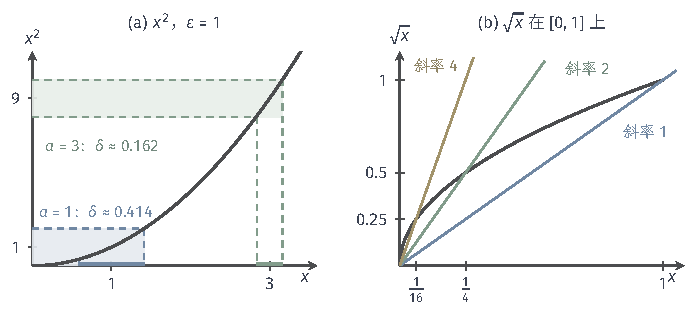
\includegraphics[width=116.695mm]{figures/02-abstract-mathematics/01-metric-and-measure/tikz/c1-uniform-continuity/figure.pdf}
  \caption{连续性中容差随位置的变化。(a) $f(x)=x^2$，取输出容差$\varepsilon=1$：在$a=1$处输入可以偏离$\sqrt2-1\approx0.414$，在$a=3$处只能偏离$\sqrt{10}-3\approx0.162$，曲线越陡，可用的输入区间越窄，在全实轴上没有统一的$\delta$。(b) $f(x)=\sqrt x$在$[0,1]$上：过点$(t,\sqrt t)$与原点的割线斜率$1/\sqrt t$在$t\to0$时无界，图中画出$t=1,\ 1/4,\ 1/16$三条割线，斜率依次为$1,\ 2,\ 4$；不存在统一的Lipschitz常数，但$\sqrt x$在$[0,1]$上仍一致连续。}
  \label{fig:metric-uniform-continuity}
\end{figure*}

\paragraph{一致连续映射保持柯西列}
若$f$一致连续而$(x_n)$是$D$中的柯西列，对$\varepsilon>0$取一致连续的$\delta$，再取$N$使$m,n\geq N$时$d_X(x_m,x_n)<\delta$，则$d_Y(f(x_m),f(x_n))<\varepsilon$，所以$(f(x_n))$是柯西列。逐点连续做不到这一点：$f(x)=1/x$在$(0,1)$上连续，柯西列$1/(n+1)$的像$n+1$却不是柯西列。另一方面，保持柯西列不等于输出有极限：恒等映射$(0,1)\to(0,1)$一致连续，柯西列$1/(n+1)$的像仍是它自己，在陪域$(0,1)$中没有极限。输出极限是否存在取决于陪域是否完备。

\subsection{Lipschitz映射}
\label{sec:metric-lipschitz}

一致连续只保证存在统一的$\delta$，没有说明$\delta$与$\varepsilon$的数量关系。很多误差估计需要更具体的结论：输出误差不超过输入误差的固定倍数。

\begin{definition}[Lipschitz映射]
\label{def:metric-lipschitz}
若存在常数$L\geq0$，使所有$x,y\in D$都满足
\[
  d_Y(f(x),f(y))\leq L\,d_X(x,y),
\]
就称$f$是\term{Lipschitz映射}（Lipschitz map），$L$称为Lipschitz常数。若每个$a\in D$都有半径$r_a>0$与常数$L_a$，使上式在$D\cap B(a,r_a)$上以$L_a$成立，就称$f$\term{局部Lipschitz}（locally Lipschitz）。
\end{definition}

全局Lipschitz推出一致连续：$L>0$时取$\delta=\varepsilon/L$，$L=0$时$f$为常值，任取$\delta$即可。局部Lipschitz推出连续：在$a$处取$\delta=\min\{r_a,\varepsilon/(L_a+1)\}$，则$d_X(x,a)<\delta$时$d_Y(f(x),f(a))\leq L_a\delta<\varepsilon$。局部常数$L_a$可以随$a$无限增大，这时没有全局常数。由反向三角不等式~\eqref{eq:metric-reverse-triangle}，对固定的$z$，$x\mapsto d_X(x,z)$是Lipschitz常数为$1$的映射；同样，由式~\eqref{eq:metric-distance-to-set}定义的$x\mapsto d_X(x,A)$也是$1$-Lipschitz的：对任意$a\in A$，$d_X(x,A)\leq d_X(x,a)\leq d_X(x,y)+d_X(y,a)$，对$a$取下确界得$d_X(x,A)\leq d_X(x,y)+d_X(y,A)$，交换$x,y$即得。

\paragraph{三种条件的区分}
两个例子说明三种条件确实不同。$\sqrt x$在$[0,1]$上一致连续：对$0\leq y\leq x$，$(\sqrt x-\sqrt y)^2\leq(\sqrt x-\sqrt y)(\sqrt x+\sqrt y)=x-y$，所以$|\sqrt x-\sqrt y|\leq\sqrt{|x-y|}$，取$\delta=\varepsilon^2$即可。但它不是Lipschitz映射：$|\sqrt t-\sqrt0|/|t-0|=1/\sqrt t$在$t\to0$时无界，见图~\ref{fig:metric-uniform-continuity}(b)。$x^2$在$\mathbb R$上局部Lipschitz：在$B(a,1)$中$|x^2-y^2|\leq(2|a|+2)|x-y|$；但例~\ref{ex:metric-square-uniform}已经说明它不一致连续，更不是全局Lipschitz。于是在固定定义域和两端度量时，
\[
  \begin{gathered}
    \text{Lipschitz}\Longrightarrow\text{一致连续}\Longrightarrow\text{连续},\\
    \text{Lipschitz}\Longrightarrow\text{局部Lipschitz}\Longrightarrow\text{连续},
  \end{gathered}
\]
各个反向蕴含都不成立。改变定义域或度量后，这些判断需要重新检查。

\subsection{紧致集上的连续映射}
\label{sec:metric-compact-continuous}

第~\ref{sec:metric-compactness}节的紧致性与本节的连续性结合，可以回答两个前面留下的问题：连续函数何时取到最值，下确界$d(x,A)$何时由最近点达到；还能说明紧致定义域上逐点连续何时升级为一致连续。

\begin{theorem}[连续像保持紧致]
\label{thm:metric-compact-image}
若$K$紧致而$f:K\to Y$连续，则$f(K)$是$Y$中的紧致集。特别地，若$K$非空，连续函数$f:K\to\mathbb R$在$K$上取得最大值和最小值。
\end{theorem}

\begin{proof}
设$\{V_\alpha\}$是$Y$中覆盖$f(K)$的一族开集。由定理~\ref{thm:metric-open-preimage}，每个$f^{-1}(V_\alpha)$是$K$中的开集，它们覆盖$K$。由紧致性，有限个$f^{-1}(V_{\alpha_i})$（$i=1,\dots,k$）覆盖$K$，于是$V_{\alpha_1},\dots,V_{\alpha_k}$覆盖$f(K)$。

对实值函数，$f(K)$是$\mathbb R$中的非空紧致集，因而有界且闭。令$s=\sup f(K)<\infty$，由上确界的性质，对每个$n$有$f(K)$中的点大于$s-1/n$，所以$s\in\overline{f(K)}=f(K)$，即存在$x^\star\in K$使$f(x^\star)=s$。最小值同理。
\end{proof}

\paragraph{最近点的存在}
对固定点$x\in X$，映射$a\mapsto d(x,a)$是$1$-Lipschitz的，因而连续。若$A$是非空紧致集，由定理~\ref{thm:metric-compact-image}，它在某个$a^\star\in A$处取到最小值，即$d(x,a^\star)=d(x,A)$：最近点存在。这回答了第~\ref{sec:metric-closure}小节的问题：在$d(2,(0,1))=1$的例子中，$(0,1)$不紧致，下确界没有达到；换成紧致的$[0,1]$，最近点$1$就存在。最近点不一定唯一：原点到单位圆周$S^1$上每一点的距离都是$1$，每一点都是最近点。

\paragraph{连续升级为一致连续}
第~\ref{sec:metric-uniform-continuity}小节中，$x^2$在$\mathbb R$上找不到统一容差，是因为基点可以无限远离原点。紧致定义域排除了这种情形。

\begin{theorem}[紧致集上的一致连续]
\label{thm:metric-compact-uniform}
若$K$紧致而$f:K\to Y$连续，则$f$在$K$上一致连续。
\end{theorem}

\begin{proof}
若不然，存在$\varepsilon>0$，使对每个$\delta=1/n$都有$x_n,y_n\in K$满足$d_X(x_n,y_n)<1/n$而$d_Y(f(x_n),f(y_n))\geq\varepsilon$。由定理~\ref{thm:metric-compact-sequential}，取子列$x_{n_k}\to x\in K$。由$d_X(y_{n_k},x)\leq d_X(y_{n_k},x_{n_k})+d_X(x_{n_k},x)\to0$，也有$y_{n_k}\to x$。由$f$在$x$处连续及序列判据，$f(x_{n_k})\to f(x)$且$f(y_{n_k})\to f(x)$，于是$d_Y(f(x_{n_k}),f(y_{n_k}))\leq d_Y(f(x_{n_k}),f(x))+d_Y(f(x),f(y_{n_k}))\to0$，与它始终不小于$\varepsilon$矛盾。
\end{proof}

这一定理给出统一的容差，但不给出Lipschitz常数：$\sqrt x$在紧致的$[0,1]$上连续，因而一致连续，却不是Lipschitz映射。它也解释了例~\ref{ex:metric-square-uniform}：$[-M,M]$紧致，$x^2$在其上一致连续；$\mathbb R$不紧致，结论不再成立。

\section{度量空间的比较}
\label{sec:metric-comparison}

上一节固定映射，研究它的连续性；本节反过来，用映射比较两个度量空间：如果两个空间之间有一个足够好的对应，一侧的柯西列、完备性和开集能否搬到另一侧？比较的强弱取决于对应保留了什么。等距与双Lipschitz映射双向控制距离的数值，同胚只要求双向连续。同一底集上的两个度量，也可以借恒等映射按这两种要求比较。

\subsection{等距与双Lipschitz映射}
\label{sec:metric-bilipschitz}

最强的比较是距离完全不变。把平面上的图形平移或旋转，所有两点距离都保持不变；把一个空间放进它的完备化，原有距离也不变。

\begin{definition}[等距与双Lipschitz映射]
\label{def:metric-bilipschitz}
设$f:D\to Y$，$D\subseteq X$。若存在常数$0<c\leq C<\infty$，使所有$x,y\in D$满足
\begin{equation}
\label{eq:metric-bilipschitz}
  c\,d_X(x,y)\leq d_Y(f(x),f(y))\leq C\,d_X(x,y),
\end{equation}
就称$f$为\term{双Lipschitz映射}（bi-Lipschitz map）。$c=C=1$，即$d_Y(f(x),f(y))=d_X(x,y)$时，称$f$为\term{等距映射}（isometry）。
\end{definition}

上界说明$f$是Lipschitz映射，控制正向误差。下界有两个作用：若$f(x)=f(y)$，则$c\,d_X(x,y)\leq0$，于是$x=y$，所以$f$是单射；并且逆映射$f^{-1}:f(D)\to D$满足$d_X(f^{-1}(u),f^{-1}(v))\leq c^{-1}d_Y(u,v)$，是常数为$1/c$的Lipschitz映射。逆映射只在实际像$f(D)$上有定义；只有当$f$还是满射时，才能说它在整个$Y$上可逆。

\begin{example}[有限维范数之间的恒等映射]
\label{ex:metric-identity-bilipschitz}
在$\mathbb R^d$上，对每个$\bm x$有$\lVert\bm x\rVert_2\leq\lVert\bm x\rVert_1\leq\sqrt d\,\lVert\bm x\rVert_2$，其中右边一式来自Cauchy--Schwarz不等式$\sum_i|x_i|\cdot1\leq\bigl(\sum_ix_i^2\bigr)^{1/2}\sqrt d$。所以恒等映射$(\mathbb R^d,d_2)\to(\mathbb R^d,d_1)$是双Lipschitz映射，$c=1$，$C=\sqrt d$。$d=2$时，取$\bm x=(1,1)$，$\lVert\bm x\rVert_1=2=\sqrt2\,\lVert\bm x\rVert_2$，上界取等号，这个常数不能再小。
\end{example}

\paragraph{双Lipschitz映射保留的性质}
由式~\eqref{eq:metric-bilipschitz}，$d_X(x_m,x_n)$与$d_Y(f(x_m),f(x_n))$同时趋于零，所以$(x_n)$是$D$中的柯西列当且仅当$(f(x_n))$是$f(D)$中的柯西列，$x_n\to x$当且仅当$f(x_n)\to f(x)$。由此，$D$完备当且仅当$f(D)$完备：若$D$完备，$f(D)$中的柯西列$(f(x_n))$对应$D$中的柯西列$(x_n)$，它收敛到某个$x\in D$，于是$f(x_n)\to f(x)\in f(D)$；反方向对逆映射作同样论证。全有界性也相互对应：$\{a_1,\dots,a_k\}$是$D$的$\varepsilon$网时，$\{f(a_1),\dots,f(a_k)\}$是$f(D)$的$C\varepsilon$网；反过来，$f(D)$的$\varepsilon$网对应$D$的$\varepsilon/c$网。这些比较都针对实际像$f(D)$；若$f$不是满射，陪域$Y$中$f(D)$以外的部分不受约束。

图~\ref{fig:metric-bilipschitz-homeo}(a)用例~\ref{ex:metric-identity-bilipschitz}中的常数画出了双Lipschitz映射的特点：输出距离被夹在两条过原点的直线之间。

\subsection{同胚与度量的比较}
\label{sec:metric-homeomorphism}

很多问题只关心收敛与开集，不关心误差的比例。例如判断一个点列是否收敛、一个集合是否开，只需知道哪些点“任意接近”，不必知道接近的速度。

\begin{definition}[同胚]
\label{def:metric-homeomorphism}
若双射$h:X\to Y$与它的逆映射$h^{-1}:Y\to X$都连续，就称$h$为\term{同胚}（homeomorphism），称$X$与$Y$同胚。
\end{definition}

由开集原像判据，同胚把$X$的开集恰好对应到$Y$的开集：$U$在$X$中开时，$h(U)=(h^{-1})^{-1}(U)$在$Y$中开，反之亦然。由序列判据，$x_n\to x$当且仅当$h(x_n)\to h(x)$。所以同胚保留开集、闭集、闭包、收敛与连续性这些只依赖开集的结构。双Lipschitz双射的两个方向都是Lipschitz映射，因而都连续，必为同胚；反之则不然，下面的例子说明同胚不必保持距离的比例。

\paragraph{同一底集上的两种度量}
若$d$与$d'$是同一集合$X$上的两个度量，恒等映射$(X,d)\to(X,d')$是同胚，当且仅当两个度量给出相同的开集；这时称两个度量\term{拓扑等价}（topologically equivalent）。若恒等映射还是双Lipschitz的，即存在$0<c\leq C$使$c\,d\leq d'\leq C\,d$，就称它们\term{强等价}（strongly equivalent）。例~\ref{ex:metric-identity-bilipschitz}说明$d_1$与$d_2$强等价；第~\ref{sec:metric-definition}节的$\rho_1$与$\rho_\infty$由式~\eqref{eq:metric-product-bounds}也强等价。而$\mathbb R$上的通常距离与离散度量不拓扑等价：$\{0\}$在离散度量下开，在通常距离下不开。这里只讨论度量诱导的开集，不展开一般拓扑空间的公理体系。

\begin{example}[logit同胚与完备性]
\label{ex:metric-logit}
令$h:(0,1)\to\mathbb R$，$h(x)=\ln\dfrac{x}{1-x}$，两端都取通常距离。它是严格单调的连续双射，逆映射是$\sigma(t)=1/(1+\mathrm e^{-t})$，也连续，所以$h$是同胚。$(0,1)$不完备，$\mathbb R$完备；同胚没有保留完备性。原因在于$h$不是双Lipschitz映射：柯西列$x_n=1/(n+1)$的像$h(x_n)=\ln\dfrac{1/(n+1)}{n/(n+1)}=-\ln n$满足$|h(x_{2n})-h(x_n)|=\ln2$，对任何$N$都有相距$\ln2$的两项，所以$(h(x_n))$不是柯西列。具体地，$h(x_1),\dots,h(x_4)$依次为$0,\ -0.693,\ -1.099,\ -1.386$，而$x_1,\dots,x_4$之间的距离越来越小。图~\ref{fig:metric-bilipschitz-homeo}(b)画出了这种拉伸：同胚保留“哪些点列收敛”，却可以把一列趋向缺失端点的柯西列拉成无界的点列。
\end{example}

\begin{figure*}[!htbp]
  \centering
  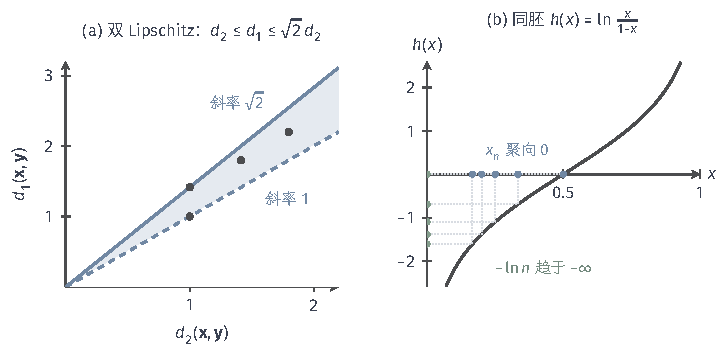
\includegraphics[width=123.261mm]{figures/02-abstract-mathematics/01-metric-and-measure/tikz/c1-bilipschitz-homeo/figure.pdf}
  \caption{双Lipschitz映射与同胚的区别。(a) 恒等映射$(\mathbb R^2,d_2)\to(\mathbb R^2,d_1)$：横轴为输入距离$d_2$，纵轴为输出距离$d_1$，所有点对都落在斜率$1$与$\sqrt2$两条直线之间的蓝色楔形中，输出误差与输入误差相差不超过常数倍。(b) logit同胚$h(x)=\ln(x/(1-x))$：横轴上的蓝点$x_n=1/(n+1)$（$n=1,\dots,5$）向$0$聚拢，构成柯西列，纵轴上的像$-\ln n$却越拉越远并趋于$-\infty$。}
  \label{fig:metric-bilipschitz-homeo}
\end{figure*}

这个例子同时说明，完备性不是只由开集决定的性质：$\mathbb R$上的通常距离$|s-t|$与$d'(s,t)=|\sigma(s)-\sigma(t)|$给出相同的开集（$\sigma:\mathbb R\to(0,1)$是同胚），但$(\mathbb R,|\cdot|)$完备，而在$d'$下点列$t_n=n$满足$d'(t_m,t_n)=|\sigma(m)-\sigma(n)|\to0$，是柯西列，却没有极限：若在$d'$下$t_n\to t$，则$\sigma(n)\to\sigma(t)<1$，与$\sigma(n)\to1$矛盾。讨论完备性、全有界性以及下一节的压缩条件时，必须指明所用的度量；只说“拓扑相同”不够。

\section{压缩映射与不动点}
\label{sec:metric-contraction}

章首的迭代$x^{(t+1)}=x^{(t)}/2+1$想求的是方程$x=x/2+1$的解。很多方程都可以写成$x=T(x)$的形式，再从一个初值出发反复应用$T$。本节把前面的工具用在同一个构造问题上：距离控制给出误差的几何衰减，柯西列与完备性给出极限的存在，连续性验证极限确实是解。然后讨论迭代应在何时停止，以及每步计算有误差时结论怎样修改。本节用带括号的上标$x^{(t)}$表示第$t$次迭代的结果。

\subsection{压缩映射定理}
\label{sec:metric-contraction-theorem}

满足$T(x^\star)=x^\star$的点$x^\star$称为$T$的\term{不动点}（fixed point）。迭代能否找到不动点，取决于$T$是否一致地拉近任意两点。

\begin{definition}[压缩映射]
\label{def:metric-contraction}
设$(X,d)$是度量空间，$T:X\to X$。若存在常数$0\leq q<1$，使所有$x,y\in X$都满足$d(T(x),T(y))\leq q\,d(x,y)$，就称$T$为\term{压缩映射}（contraction mapping），$q$称为压缩常数。
\end{definition}

压缩映射是Lipschitz常数小于$1$的自映射：它把$X$映回$X$自身，所以迭代可以无限进行下去；它对所有点对使用同一个$q$，所以每一步都至少把距离缩小到原来的$q$倍。

\begin{theorem}[压缩映射定理]
\label{thm:metric-contraction}
设$(X,d)$是非空完备度量空间，$T:X\to X$是压缩常数为$q$的压缩映射。则$T$有唯一的不动点$x^\star$，并且对任意初值$x^{(0)}\in X$，迭代$x^{(t+1)}=T(x^{(t)})$收敛到$x^\star$。
\end{theorem}

\begin{proof}
\emph{相邻差几何衰减。}由压缩条件，
\[
  d(x^{(t+1)},x^{(t)})=d\bigl(T(x^{(t)}),T(x^{(t-1)})\bigr)\leq q\,d(x^{(t)},x^{(t-1)}),
\]
反复使用得到$d(x^{(t+1)},x^{(t)})\leq q^t\,d(x^{(1)},x^{(0)})$。

\emph{迭代列是柯西列。}对$s>t$，沿中间各项用三角不等式，再对几何级数求和：
\begin{equation}
\label{eq:metric-contraction-tail}
  \begin{aligned}
    d(x^{(s)},x^{(t)})&\leq\sum_{k=t}^{s-1}d(x^{(k+1)},x^{(k)})
    \leq\sum_{k=t}^{s-1}q^k\,d(x^{(1)},x^{(0)})\\
    &\leq\frac{q^t}{1-q}\,d(x^{(1)},x^{(0)}).
  \end{aligned}
\end{equation}
因为$0\leq q<1$，右边在$t\to\infty$时趋于零，且与$s$无关，所以$(x^{(t)})$是柯西列。

\emph{极限存在且是不动点。}$X$完备，所以存在$x^\star\in X$使$x^{(t)}\to x^\star$。压缩映射是Lipschitz映射，因而连续，由序列判据$T(x^{(t)})\to T(x^\star)$。而$T(x^{(t)})=x^{(t+1)}\to x^\star$，由极限唯一，$T(x^\star)=x^\star$。

\emph{唯一性。}若$T(y^\star)=y^\star$，则$d(x^\star,y^\star)=d(T(x^\star),T(y^\star))\leq q\,d(x^\star,y^\star)$，即$(1-q)\,d(x^\star,y^\star)\leq0$。由$q<1$，$d(x^\star,y^\star)=0$，$x^\star=y^\star$。
\end{proof}

对$T(x)=x/2+1$，在$\mathbb R$上$|T(x)-T(y)|=|x-y|/2$，$q=1/2$，$\mathbb R$完备，所以有唯一不动点；解$x=x/2+1$得$x^\star=2$。从$x^{(0)}=0$出发，迭代依次为$0,\ 1,\ 1.5,\ 1.75,\ 1.875,\ 1.9375,\dots$，误差$|x^{(t)}-2|=2^{1-t}$每步减半。图~\ref{fig:metric-contraction}(a)用蛛网图画出了这个过程：在$y=T(x)$与$y=x$之间来回走折线，折线逐步收拢到两线的交点。

\paragraph{各条件的职责}
定理的四个条件各有作用，缺一不可。非空保证有初值可取。自映射保证每次迭代都留在$X$中。完备性提供极限：$T(x)=x/2$作为$(0,1)\to(0,1)$的映射满足$q=1/2$，迭代$x^{(t)}=2^{-t}x^{(0)}$是柯西列，但它在$\mathbb R$中的极限$0$不在$(0,1)$中，$T$在$(0,1)$上没有不动点。统一的$q<1$提供几何衰减：平移$T(x)=x+1$满足$|T(x)-T(y)|=|x-y|$，常数等于$1$，在完备的$\mathbb R$上却没有不动点。仅仅“相邻距离逐渐变小”也不够：$x^{(t)}=\sum_{k=1}^t1/k$的相邻差$1/(t+1)$趋于零，点列却趋于无穷，因为相邻差之和发散；压缩条件保证的是相邻差按几何级数衰减，其和有限。

\subsection{迭代误差与停止条件}
\label{sec:metric-contraction-error}

实际计算只能进行有限步，需要在不知道$x^\star$的情况下判断当前结果有多准确。证明中的几何尾和给出了答案。

\paragraph{先验与后验误差界}
在式~\eqref{eq:metric-contraction-tail}中令$s\to\infty$。由$d(\cdot,x^{(t)})$的连续性，左边趋于$d(x^\star,x^{(t)})$，于是得到\term{先验误差界}（a priori error bound）
\begin{equation}
\label{eq:metric-a-priori}
  d(x^{(t)},x^\star)\leq\frac{q^t}{1-q}\,d(x^{(1)},x^{(0)}).
\end{equation}
它只用第一步的位移，迭代开始前就能算出达到给定精度所需的步数。若把第$t-1$步看作新的初值，同一个估计给出$d(x^{(t)},x^\star)\leq\dfrac{q}{1-q}\,d(x^{(t)},x^{(t-1)})$，称为\term{后验误差界}（a posteriori error bound）
\begin{equation}
\label{eq:metric-a-posteriori}
  d(x^{(t)},x^\star)\leq\frac{q}{1-q}\,d(x^{(t)},x^{(t-1)}).
\end{equation}
它使用当前的相邻差，迭代过程中可以随时检查。

\begin{example}[按目标精度停止]
\label{ex:metric-contraction-stop}
对$T(x)=x/2+1$、$x^{(0)}=0$，有$q=1/2$、$d(x^{(1)},x^{(0)})=1$，先验界为$2^{1-t}$。要求误差不超过$10^{-3}$，需要$2^{t-1}\geq1000$；由$2^9=512<1000\leq1024=2^{10}$，取$t=11$，此时$x^{(11)}=1.9990234375$，误差$2^{-10}\approx0.000977$。后验界的系数$q/(1-q)=1$，例如$t=5$时$d(x^{(5)},x^{(4)})=1.9375-1.875=0.0625$，后验界为$0.0625$，而实际误差$|1.9375-2|=0.0625$。这个线性例子中两个误差界都恰好取等号。
\end{example}

\paragraph{收缩缓慢时的停止判断}
后验界中的系数$q/(1-q)$在$q$接近$1$时很大，小的相邻差可能对应大的误差。取$T(x)=0.99x+1$，它在$\mathbb R$上是$q=0.99$的压缩映射，不动点为$x^\star=100$。从$x^{(0)}=0$出发，$x^{(t)}=100(1-0.99^t)$，相邻差$d(x^{(t+1)},x^{(t)})=0.99^t$。当$t=459$时相邻差约为$0.00992$，首次小于$0.01$；而此时$x^{(460)}$的误差$100\cdot0.99^{460}\approx0.982$，几乎是相邻差的$99$倍，与后验界一致。若只凭“相邻两次变化小于$0.01$”就停止，结果会差将近$1$。先验界$100\cdot0.99^t\leq10^{-3}$要求$t\geq\ln(10^{-5})/\ln0.99\approx1145.5$，即约$1146$步，而$q=1/2$时只需$11$步。两个例子都满足定理的全部条件，定理保证收敛，却不保证收敛得快。

\subsection{带误差的压缩迭代}
\label{sec:metric-inexact-contraction}

实际计算中，$T(x^{(t)})$往往只能近似求出，例如受浮点舍入或内层迭代截断的影响。设精确映射$T$仍满足压缩条件，而实际得到的$x^{(t+1)}\in X$满足
\[
  d(x^{(t+1)},T(x^{(t)}))\leq\eta_t,
\]
其中$\eta_t\geq0$是第$t$步的执行误差。近似点必须仍在$X$中，否则压缩条件无从使用。

\paragraph{误差递推}
令$e_t=d(x^{(t)},x^\star)$。由三角不等式与$T(x^\star)=x^\star$，
\[
  e_{t+1}\leq d(x^{(t+1)},T(x^{(t)}))+d(T(x^{(t)}),T(x^\star))\leq\eta_t+q\,e_t.
\]
反复代入得到
\begin{equation}
\label{eq:metric-inexact-error}
  e_t\leq q^t e_0+\sum_{s=0}^{t-1}q^{t-1-s}\eta_s.
\end{equation}
第一项是初始误差的几何衰减，与精确迭代相同；第二项是各步新引入的误差，它们被后续步骤按$q$的幂次逐渐压缩，但不会消失。

\begin{theorem}[带误差的压缩迭代]
\label{thm:metric-inexact-contraction}
在上述设定下：(1) 若$\eta_t\leq\eta$对所有$t$成立，则$e_t\leq q^te_0+\eta/(1-q)$，从而$\limsup_{t\to\infty}e_t\leq\eta/(1-q)$；(2) 若$\eta_t\to0$，则$e_t\to0$，即$x^{(t)}\to x^\star$。
\end{theorem}

\begin{proof}
(1) 在式~\eqref{eq:metric-inexact-error}中把每个$\eta_s$放大为$\eta$，得到$\sum_{s=0}^{t-1}q^{t-1-s}\eta\leq\eta\sum_{k=0}^\infty q^k=\eta/(1-q)$。再令$t\to\infty$，$q^te_0\to0$。

(2) 设$\varepsilon>0$，取$S$使$s\geq S$时$\eta_s<\varepsilon$。对$t>S$，把和式分成$s<S$与$s\geq S$两段：
\[
  \sum_{s=0}^{t-1}q^{t-1-s}\eta_s
  \leq q^{t-S}\sum_{s=0}^{S-1}\eta_s+\varepsilon\sum_{k=0}^{\infty}q^k
  =q^{t-S}\sum_{s=0}^{S-1}\eta_s+\frac{\varepsilon}{1-q},
\]
其中第一段用了$s<S$时$q^{t-1-s}\leq q^{t-S}$。$S$固定后，第一项在$t\to\infty$时趋于零，所以$\limsup_te_t\leq\varepsilon/(1-q)$。$\varepsilon$任意，故$e_t\to0$。
\end{proof}

\begin{example}[固定执行误差]
\label{ex:metric-inexact-example}
对$T(x)=x/2+1$，设每步实际计算$x^{(t+1)}=T(x^{(t)})+0.1$，即$\eta_t=0.1$。从$x^{(0)}=0$出发，迭代依次为$0,\ 1.1,\ 1.65,\ 1.925,\ 2.0625,\ 2.13125,\dots$，收敛到$x/2+1.1=x$的解$2.2$，与精确不动点$2$相差$0.2$。定理~\ref{thm:metric-inexact-contraction}(1)给出的界$\eta/(1-q)=0.1/(1/2)=0.2$在这里恰好达到。图~\ref{fig:metric-contraction}(b)比较了精确迭代与带误差迭代的误差：前者每步减半，后者先下降，再停在$0.2$附近。
\end{example}

\begin{figure*}[!htbp]
  \centering
  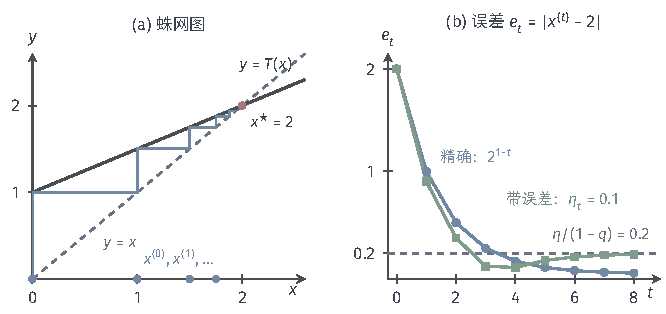
\includegraphics[width=112.691mm]{figures/02-abstract-mathematics/01-metric-and-measure/tikz/c1-contraction/figure.pdf}
  \caption{压缩迭代$T(x)=x/2+1$，初值$x^{(0)}=0$。(a) 蛛网图：从$x^{(0)}$出发竖直走到曲线$y=T(x)$，再水平走到对角线$y=x$，得到下一个迭代值；折线收拢到交点$x^\star=2$。(b) 误差$e_t=|x^{(t)}-2|$：蓝色为精确迭代，$e_t=2^{1-t}$；绿色为每步加入执行误差$0.1$的迭代，误差先下降，越过精确解后趋向$0.2$；灰色虚线是误差上界$\eta/(1-q)=0.2$。}
  \label{fig:metric-contraction}
\end{figure*}

\paragraph{带误差时的停止判断}
执行误差也改变停止判断。对任意$x\in X$，$d(x,x^\star)\leq d(x,T(x))+d(T(x),T(x^\star))\leq d(x,T(x))+q\,d(x,x^\star)$，所以$d(x,x^\star)\leq d(x,T(x))/(1-q)$。取$x=x^{(t)}$，并用$d(x^{(t)},T(x^{(t)}))\leq d(x^{(t)},x^{(t+1)})+\eta_t$，得到
\[
  e_t\leq\frac{d(x^{(t+1)},x^{(t)})+\eta_t}{1-q}.
\]
可观测的相邻差必须连同本步执行误差一起判断：在上例中，迭代停在$2.2$附近时相邻差趋于零，但$\eta_t=0.1$使右边始终不小于$0.2$，正确地提示结果并没有比$0.2$更准。本节只保留这一通用机制；线性方程组的迭代解法和最优化中的迭代算法，会在相应部分利用具体结构给出压缩常数。

\section{本章小结}
\label{sec:metric-summary}

本章从实数的绝对值、向量的范数、二进制串的Hamming距离和图的最短路距离中提炼出度量的三条要求，并说明度量是空间结构的一部分：同一集合换一个度量，球的形状、哪些点列收敛、是否可分都可能改变。距离依次提供了三层语言。开球给出邻近结构，由它定义开集、闭集、闭包与稠密；点列收敛把邻近变成可以逐项检查的误差，闭集的序列判据把两者连起来；连续映射研究误差在两个空间之间的传递，一致连续与Lipschitz条件分别要求统一的容差与统一的放大倍数。

几个“有限性”与“存在性”条件分别控制不同的对象。有界控制集合的总体范围；可分要求一套可数代表服务所有精度；全有界要求每个精度只需有限个代表；完备要求柯西列在空间内有极限；紧致要求每个给定的开覆盖都有有限子覆盖。在度量空间中，紧致等价于序列紧致，也等价于完备且全有界；只有在$\mathbb R^d$这样的有限维欧氏空间中，才可以简化为闭且有界。紧致定义域使连续函数取得最值、使最近点存在、使连续升级为一致连续，但不提供Lipschitz常数。比较两个空间时，双Lipschitz映射保留柯西列、完备性和全有界性，同胚只保留开集与收敛；logit映射表明，完备性不是由开集单独决定的。

压缩映射定理把这些结论串成一条完整的论证：统一的压缩常数使相邻差几何衰减，几何尾和使迭代列成为柯西列，完备性给出极限，连续性验证极限满足$T(x^\star)=x^\star$，压缩条件再给出唯一性。同一条尾和估计给出先验与后验误差界，带误差的版本说明执行误差会留下$\eta/(1-q)$量级的偏差。各个反例提醒我们：只观察到相邻项越来越近，或在局部看到误差缩小，都不足以断定极限存在或结果准确；每个结论都需要它的全部条件。

下一章转向另一个问题：怎样测量一个集合的大小。度量空间的开集将生成Borel集合族，为测量提供可用的集合；但距离本身并不决定集合的测度，同一个度量空间上可以有许多不同的测度。


\chapter{测度空间}
\label{chap:measure-spaces}

在前面的微积分里，我们累计一个量时，底集总是实轴或欧氏空间：长度、面积、体积已经替我们规定好“一块区域有多大”，积分就是在这套规定上累计函数。
但在机器学习中，需要累计的对象往往不是数：它们可能是词、类别、图、数据样本，或者另一个空间里的点。
这时长度和体积帮不上忙，我们必须自己回答两件事——哪些集合允许被测量，以及测量的结果是多少。
回答这两个问题的工具，就是\emph{可测结构}和\emph{测度}。

读到这里很容易把“测度”和前一章的“度量（距离）”混为一谈，因为两者都在描述空间的“大小”，名字也只差一个字。
它们其实回答完全不同的问题，最好一开始就分清楚。
\emph{度量}吃进去的是\emph{两个点}，吐出来一个距离$d(x,y)$：它衡量两点隔多远，输入空集或一个集合时没有意义，而且要求$d(x,y)=d(y,x)$、$d(x,x)=0$。
\emph{测度}吃进去的是\emph{一个集合}，吐出来这个集合的“份量”$\mu(A)$：区间给长度、一群点给总权重，但它对“两点之间多远”完全不说话。
一句话对比：度量回答“$x$和$y$离得多近”，测度回答“集合$A$有多重”。
同一个点集上可以先任选一个度量、再任选一个测度，两者互不决定——例如在实轴上，标准距离配上计数测度，或者把常走的两点间距离改小而长度测度不变，都是完全合法的。
本章的“可测空间/测度空间”只需要第一层（集合的份量）；等到讨论Wasserstein距离、开球和紧性时，才在测度之外\emph{另外}加一个度量。

\begin{figure*}[htbp]
\centering
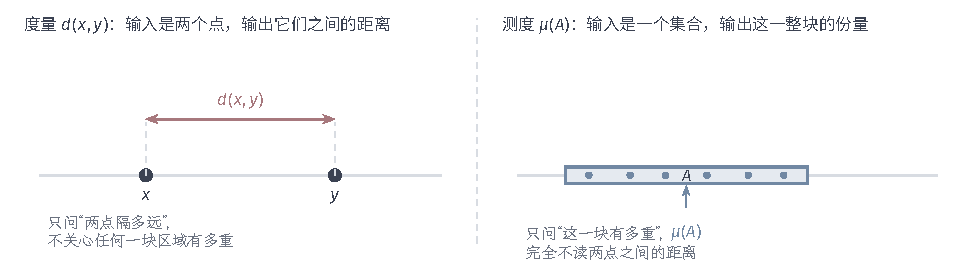
\includegraphics[width=169mm]{figures/00-shared/mathematical-preliminaries-upper/05-space-and-geometry/tikz/measure-vs-metric/figure.pdf}
\caption{度量与测度回答的是两个不同问题。度量$d(x,y)$以两个点为输入，给出它们之间的距离，并要求对称、$d(x,x)=0$、三角不等式；测度$\mu(A)$以一个集合为输入，给出这一整块的份量，并要求空集为零、可数可加。同一底集上度量与测度可以各自独立选择，互不决定。}
\label{fig:measure-vs-metric}
\end{figure*}

先看一个具体场景。
给定一批数据上的两种分布，我们会问：它们是不是一回事？如果不是，差在什么地方？
有时两种分布描述的是同一组对象，只是各部分占的比重不同：比如同一批人按两种口径统计收入。
有时它们根本描述不同空间的对象：比如一张图片和它的类别标签，需要一条规则说明图片上的“质量”怎样传到标签上。
这两类问题构成本章的两条主线。

第一条主线固定同一个空间，只比较上面的两种赋权。
我们要判断一种赋权认为是零的集合，另一种是否也认为是零；能不能找到一个密度函数，用一种赋权把另一种表示出来；以及用一个数概括两者的整体差异时，不同指标各在衡量什么。
第二条主线允许空间不同。
给定一个映射时，输入空间的质量怎样“推”到输出空间；当一个输入不只对应一个确定输出，而是按某种概率分散到若干输出时，这种规则怎样描述；如果还想知道输入与输出是怎样配对的，又要付出什么跨空间的移动代价。

\ref{sec:measure-general-structure}节先打基础，把实轴上已经熟悉的可测集合、测度、积分和乘积推广到一般空间。
\ref{sec:measure-same-space-comparison}节回到第一条主线，比较同一空间上的测度。
\ref{sec:measure-cross-space}节处理第二条主线，研究映射、测度核、联合测度和跨空间运输。
\ref{sec:measure-convergence}节再让测度随序号或时间变化，讨论一列测度怎样才算趋近、在什么条件下一定能找到收敛的子列。

这些内容不是几种互不相干的“测度种类”，而是同一套工具在回答不同问题。
确定映射其实是一种特殊的测度核：它给每个输入指派的输出测度全部集中在一个点上。
全变差、Wasserstein等差异指标也有联系：有的只看同一事件上的质量差，有的还关心两点在空间中隔得多远，我们会在相应位置把关系讲清。
概率测度在本章只是总质量恰好为$1$的测度；条件期望、Bayes公式、随机过程等需要额外概率结构的内容都留给后文，这里只建立可以反复调用的通用对象和运算。

\section{一般测度的结构与积分}
\label{sec:measure-general-structure}

在实轴和欧氏空间上，“一块区域有多大”是由长度、面积、体积直接给出的。
换到一般对象的集合后，这种天然的大小不存在了，我们要自己把测量的规则补回来。
本节做四件准备工作：先说清哪些集合允许被测量、再说明怎样给这些集合配质量；然后引入开集、闭集等拓扑概念在测量中的位置；接着把熟悉的积分搬到一般测度上；最后处理两个空间的联合结构。
这些内容在实轴上都已经出现过，这里不重复证明，重点是看清“换了底集以后，哪些结论原封不动，哪些条件必须重新声明”。

\subsection{可测结构与基本赋权}

拿到一个由任意对象组成的集合后，测量要分两步走，而且两步互不相干。
第一步决定\emph{哪些集合看得见、可以测量}，这是可测结构；第二步决定\emph{看得见的集合各自有多大}，这是测度。
同一套可见集合上可以配完全不同的质量，同一个质量的想法在更粗或更细的可见范围下也要分别讨论。
本小节先建立这两层，再给出点质量、测度混合和零测例外的说法。

\subsubsection{可测范围与子$\sigma$代数}

\paragraph{可测空间与生成结构}

设$X$是我们关心的全部对象，例如若干类别、若干样本或若干状态。
要测量它的子集，先要圈定一个“允许测量的集合族”。
为什么不能直接宣布所有子集都可测？
在实轴上已经看到，一旦允许不可数次地分割、覆盖和取极限，就会出现无法自洽赋长度的集合；因此允许范围必须满足一定封闭性，但又不能大到没有限制。

我们沿用$\sigma$代数的要求：集合族$\mathcal A\subseteq\mathcal P(X)$包含全集$X$，并且对相对补集和可数并封闭。
取补和可数并还自动带来另外几种封闭：空集属于$\mathcal A$，可数交
\[
 \bigcap_nA_n=X\setminus\bigcup_n(X\setminus A_n)
\]
属于$\mathcal A$，两个可测集的差$A\setminus B=A\cap(X\setminus B)$也属于$\mathcal A$。
换句话说，凡是能用可测集合作可数多次集合运算得到的集合，仍然允许测量。
配备了这样一个集合族以后，二元组$(X,\mathcal A)$称为\term{可测空间}（measurable space），$\mathcal A$中的集合称为\term{可测集合}（measurable set）。

实际问题里，我们往往只先点名少数几个必须能测量的集合，例如区间、矩形或某些类别，其余集合由它们“生成”。
对一族集合$\mathcal C$，包含它的$\sigma$代数可能有很多，其中最小的一个记为$\sigma(\mathcal C)$。
最小性可以这样理解：幂集$\mathcal P(X)$总是一个包含$\mathcal C$的$\sigma$代数，所有这种$\sigma$代数的交仍然包含$X$且对补集、可数并封闭，所以交出来的最小范围确实存在。
这种“只规定少数起点，再封闭出全部可测集”的做法非常省事：后面验证一个映射是否可测、两项测度是否相同，都只需在起点集合上检查，再由封闭性推广到整个$\sigma$代数。

用一个有限例子体会“可见”的含义。
在$X=\{1,2,3,4\}$上，幂集$\mathcal P(X)$允许区分每一个点；但由划分$\bigl\{\{1,2\},\{3,4\}\bigr\}$生成的$\sigma$代数只有
\[
 \bigl\{\varnothing,\{1,2\},\{3,4\},X\bigr\}.
\]
在这套范围里，“第$1$个点”单独是看不见的，能测量的只有前两个点、后两个点这两个分块。
可见集合的多少，决定了我们能在多大精度上讨论问题。

\paragraph{子$\sigma$代数与同一底集上的粗化}

有时底集不变，但我们主动“眯起眼睛”，只看其中一部分集合。
若$\mathcal G\subseteq\mathcal A$本身也是一个$\sigma$代数，就称它为\term{子σ代数}。
$(X,\mathcal G)$中的对象一个不少，仍是原来的$X$，只是可见的集合变少了。
这种操作叫粗化，它和“把底集缩小成子集$Y\subseteq X$”不同：缩小底集是扔掉一批对象，粗化只是降低对同一批对象的分辨能力。

仍以四点集合为例。
在$\mathcal A=\mathcal P(X)$下四个单点都能单独测量；换成
\[
 \mathcal G=\{\varnothing,\{1,2\},\{3,4\},X\},
\]
就只能称“前两点合起来多重”“后两点合起来多重”，再也无法分开第$1$点和第$2$点。
若原来在$\mathcal A$上有测度$\mu$，只在$\mathcal G$上读取它，记作$\mu|_{\mathcal G}$，这只是缩小赋权规则的定义域，并没有删除任何点。
后面讨论\term{条件积分}时，会专门研究“在只能看到$\mathcal G$的情况下，怎样保留各分块上的累计信息”；这里先把粗化这种结构本身建立起来。

\subsubsection{测度、混合与零测例外}

\paragraph{一般测度及有限性条件}

圈定可见集合以后，就要给每个集合配一个非负的“大小”。
设$\mu$把每个可测集映到$[0,+\infty]$。
要求它满足两条：空集的大小为$0$；把互不相交的可数个集合合并时，总大小等于各部分大小之和，即
\[
 \mu\!\left(\bigcup_{n=1}^{\infty}A_n\right)=\sum_{n=1}^{\infty}\mu(A_n).
\]
这样的$\mu$称为\term{测度}（measure），$(X,\mathcal A,\mu)$称为\term{测度空间}（measure space）。
第二条（可数可加）是测量的核心：它保证“分成几块分别称，再合起来称”，结果一致。
底集换成一般对象后，这个直觉与长度完全相同；由它还能立刻得到单调性$A\subseteq B\Rightarrow\mu(A)\leq\mu(B)$和可数次可加，证明与实轴上一样，不再重复。

后面的定理对“总质量有多大”有不同要求，这里先把三个常用名词一次分清，免得以后混淆。
若$\mu(X)<\infty$，称$\mu$为\term{有限测度}；进一步若$\mu(X)=1$，称$\mu$为\term{概率测度}，此时每个集合的质量都在$[0,1]$内。
还有一个更弱、却非常常用的条件叫$\sigma$有限，满足它的测度即\term{σ有限测度}：可以用可数个可测集$E_k$盖住$X$，使每一块的质量都有限。
三者关系是：概率测度一定有限，有限测度一定$\sigma$有限（取$E_1=X$），但反过来不成立。
自然数集上的\term{计数测度}（counting measure）给每个点质量$1$、全空间质量无穷，却能被单点集$\{1\},\ldots,\{k\}$有限地盖住；实轴上的勒贝格测度总质量无穷，但区间$[-k,k]$每一块都有限——它们都是$\sigma$有限而不有限。

集合列的连续性沿用前面的结论，但要留意有限性出现在哪里。
集合逐渐扩大时，$A_n\uparrow A$就有$\mu(A_n)\uparrow\mu(A)$，不要求任何有限性；集合逐渐缩小时，$A_n\downarrow A$要得到$\mu(A_n)\downarrow\mu(A)$，必须先有$\mu(A_1)<\infty$。
否则$(n,\infty)\downarrow\varnothing$，而每一项的勒贝格长度都是无穷，无法相减得到零。
请记住：$\sigma$有限不是所有运算的万能前提，密度表示、乘积构造和有界函数积分各自需要的条件，会在用到时分别说明。

\paragraph{加权点测度与\term{可数混合}}

最容易想象的测度，是把质量直接放在若干个点上。
固定一个点$x$（并假设$\{x\}$可测），定义
\[
 \delta_x(A)=\mathbf 1_A(x)=
 \begin{cases}1,&x\in A,\\0,&x\notin A,\end{cases}
\]
称为集中在$x$的\term{点质量}（point mass）：集合包含$x$就得质量$1$，否则得$0$。
它对应“全部重量压在一个点上”的极端赋权。

再取一列点$x_i$和非负权重$w_i\geq0$，把若干点质量加起来：
\[
 \mu=\sum_i w_i\delta_{x_i},\qquad
 \mu(A)=\sum_i w_i\,\mathbf 1_A(x_i).
\]
因为每个点属于哪些不交集合是唯一确定的，两个非负求和可以交换次序，所以$\mu$仍然可数可加；同一位置上的权重自动相加。
权重总和有限时$\mu$是有限测度，总和为$1$时就是概率测度。
这里有个细节：定义本身不要求每个单点都可测，但只要具体计算中用到$\delta_x(\{x\})=1$，就必须先确认$\{x\}\in\mathcal A$。

同样的“加权相加”还可以用在测度上。
设$\mu_i$是同一空间上的非负测度，取非负系数$a_i$，令
\[
 \mu(A)=\sum_i a_i\mu_i(A),
\]
非负级数换序保证$\mu$仍是测度。
若各$\mu_i$都是概率测度且系数和为$1$，得到的就是可数混合：以比例$a_i$在第$i$种随机规律之间随机挑选一种。
一个直观例子是
\[
 \mu=\tfrac12\,\lambda|_{[0,1]}+\tfrac12\delta_0:
\]
一半重量像水一样均匀铺在$[0,1]$上按长度分配，另一半重量全部压在点$0$上。
这样的混合提醒我们：一个测度完全可以同时拥有“连续铺开”的部分和“集中成点”的部分。

\paragraph{零测例外与完备化}

测量时，质量为零的集合允许我们忽略其中点上的例外。
可测集$N$若满足$\mu(N)=0$，称为零测集；某性质$\mu$几乎处处成立，是指不满足性质的点全部能装进某个可测零测集。
但“可以忽略”永远是相对于具体测度而言的：在勒贝格测度下单点$\{0\}$质量为零，可以忽略；在$\delta_0$下它的质量却是$1$，恰好是唯一重要的点。
还要注意例外能够合并的规模：可数个零测集的并仍是零测集，所以可数多个“几乎处处成立”的结论可以共用一个例外范围；不可数个零测集的并则没有这种保证。

另一个相关的性质是完备性。
若每个可测零集的任意子集都仍然可测，就称这个测度空间完备。
不完备时，可能有一个集合包含在零测集里，它本身却不可测——我们知道它“应当质量为零”，却无法在规则内给它赋值。
补救办法是完备化：把这些缺失的零测子集、以及它们与原可测集的并全部补进可测范围，并按外面的零包络赋零。
补进去以后，原来集合的测量值一个都不变，只是可测范围成为满足要求的最小扩展。
实轴上的具体构造前一章已经做过，这里只需理解它的作用：有了完备化，在零测集上随意改动一个函数的值，得到的函数仍然可测；否则“几乎处处相同”的两个函数可能一个可测、一个不可测。
因此使用几乎处处等价的函数时，要么挑一个可测的代表来用，要么明确进入完备化空间，不能简单地以为“反正是零测，怎样都行”。

\subsection{测度与拓扑结构}

仅有可测结构时，我们知道一个集合能否测量，却说不清它是开是闭、是远是近。
后面比较测度时，有些指标（例如全变差）完全不需要位置信息，另一些指标（例如Wasserstein）则必须知道两点之间的距离。
本小节把这两类条件分开：先说明开集怎样进入可测结构，再定义“测度集中在哪里”的\term{支持}。

\subsubsection{Borel结构与标准Borel范围}

\paragraph{从开集生成Borel结构}

当$X$本身带有拓扑（从而能谈开集、闭集）时，最自然的可测范围是让所有开集都可测，再封闭出其余集合。
这个由全体开集生成的$\sigma$代数称为Borel结构：
\[
 \mathcal B(X)=\sigma(\{U\subseteq X:U\text{ 是开集}\}).
\]
于是开集、闭集以及对它们作可数并、可数交、取补得到的集合都可测。
在实轴上，开区间都是开集，这个定义与前一章“由开区间生成$\mathcal B(\mathbb R)$”完全一致。
在离散空间里每个单点本身就是开集，所以Borel结构等于幂集；实轴的Borel结构却不等于全部子集，不可测集依然存在。
请特别注意：选定Borel结构只决定了“哪些集合可测”，它本身\emph{没有指定任何测度}；同一个$\mathcal B(\mathbb R)$上既可以放长度，也可以放正态分布或一个点质量。

选定一个\term{Borel测度}后再做完备化，可测范围还可能扩大。
例如勒贝格可测集族$=$实轴Borel集族$+$所有勒贝格零集的子集，比Borel结构更大。
因此要分清三个层次：拓扑规定开集，Borel$\sigma$代数由开集生成，完备化还要依赖具体选了哪个测度。
后文说“在标准Borel空间上成立”时，指的是中间这一层；不能不加核对地把完备化后才出现的集合代进去。

\paragraph{\term{Polish空间}与\term{标准Borel空间}}

后面的距离比较和测度分解经常需要一个“足够规整、又足够常见”的舞台，为此引入两个条件。
一个拓扑空间若既能找到可数个点稠密地铺在其中（可分，因而开集可以由可数个基本邻域拼出），又能配上一个与拓扑相容的完备度量（柯西列的极限仍落在空间内），就称为Polish空间。
这两个条件各有各的用处，用$\mathbb R$就能体会：可分保证我们谈论开集时只需一张可数的“基本邻域清单”（例如有理端点的开区间），不必面对不可数个无法逐个编号的邻域；完备保证“越走越近的点列”确实收敛到空间里的某个点，而不是收敛到空间外的一个“窟窿”。
本章用到\term{Wasserstein距离}时，就直接在“给定度量完备且可分”的空间上工作。
这两个条件谁也代替不了谁，更不可能仅仅因为“存在Borel$\sigma$代数”就自动成立：有理数集$\mathbb Q$可分但不完备（有理数列可以逼近无理数），反过来也存在完备但不可分的度量空间。

可测结构之间也能谈“本质相同”。
若双射$h:(X,\mathcal A)\to(Y,\mathcal B)$把可测集映成可测集、且可测集的原像也都可测，也就是每个$B\in\mathcal B$有$h^{-1}(B)\in\mathcal A$、每个$A\in\mathcal A$有$h(A)\in\mathcal B$，则称$h$为\term{可测同构}。
它表示两边的“可测拼图”能一一对应地拼回去，不要求保持距离或其他几何性质。
若一个可测空间能与某个Polish空间的Borel空间可测同构，就称它为标准Borel空间。
实数、欧氏空间、有限或可数离散空间，以及Polish空间的Borel子集都是常见例子。
这里只陈述这一范围并直接使用，不证明其分类定理。
关键直觉是：标准Borel保证“测度上的拼图足够规整”，后面的测度分解等结论可以用；但它不指定距离，也不保证你随手选的距离完备，几何比较仍要另给度量。

\subsubsection{支持与\term{全支撑}}

知道一个测度在哪些集合上有质量后，还想直观地说出“质量集中在空间的哪一片”。
支持就是这个“质量所在地”的精确说法，它还能解释连续函数的几乎处处相等等价于什么。

\paragraph{邻域定义的支持及其全质量}

对可分度量空间上的有限Borel测度$\mu$，定义
\[
 \operatorname{supp}\mu
  =\{x\in X:\text{每个包含 }x\text{ 的开邻域 }U\text{ 都有 }\mu(U)>0\}.
\]
换句话说，支持里的点“走到多近都躲不开质量”；支持外的点则存在一个开邻域完全没有质量。
正因为支持外的点各自被一个零质量开邻域包住，这些邻域的并仍是开集，所以支持是闭集。
支持必须由邻域定义，而不能简单说成“正质量单点的集合”——连续分布下每个单点质量都是零，支持却可以是整个区间。

支持还几乎承载了全部质量。
利用可分性给出的可数拓扑基$\{V_j\}$：对支持外的每个点，先取一个零质量开邻域，再从中选出一个包含该点的基开集。
这样支持外的全部点就被可数个零质量基开集盖住，由可数次可加性，
\[
 \mu(X\setminus\operatorname{supp}\mu)=0.
\]
这一步“先用可数基把任意覆盖变成可数覆盖”不能省略——直接把不可数个零测开集相加是不合法的。
作为对照：均匀分布在$[0,1]$上的测度，每个单点质量都是零，支持却是整个$[0,1]$；$\delta_0$每个邻域只有在含$0$时才有质量，支持就是$\{0\}$。
支持、正质量单点的集合、以及任意一个质量为全重的集合，是三个不同概念，不要混为一谈。

\paragraph{全支撑与连续函数的逐点辨认}

若支持扩到整个空间，$\operatorname{supp}\mu=X$，等价于每个非空开集都有正质量，称$\mu$具有全支撑。
这个条件有一个很实用的推论：在全支撑下，两个连续函数若几乎处处相等，就处处相等。
反证很直接。设连续函数$f,g$几乎处处相等，却在$x_0$处不同。
连续性保证差值$|f-g|$在$x_0$的某个开邻域$U$内仍然严格为正；全支撑又给$\mu(U)>0$。
于是$f\neq g$的地方有正质量，与几乎处处相等矛盾。
这说明：把连续函数看成“只差零测集”的等价类时，全支撑能帮我们找回逐点唯一的代表。

没有全支撑时结论就要打折扣。
在$\delta_0$下，$f(x)=x$与$g(x)=0$几乎处处相等（它们只在$x=0$以外不同，而那里没有质量），却显然不是同一个函数。
一般地，只要在支持上连续且相等，就足以推出几乎处处相等；但要想把结论恢复到整个空间的每一个点，才需要全支撑这类额外条件。

\subsection{一般积分的适用条件}

积分的构造思想在一般测度上并不改变：先在取值简单的函数上按集合质量加权，再用简单函数逼近一般函数。
本小节只回答三个问题：函数满足什么条件才能与可测结构配合、积分什么时候是有限实数、以及前一章的三条积分极限定理在一般空间还成不成立。

\subsubsection{\term{可测映射}与积分条件}

\paragraph{原像判据与可测复合}

函数或映射要参与测量，先要保证它不会把输出端的可测事件拉回输入端的不可测集合。
设$f:(X,\mathcal A)\to(Y,\mathcal B)$，若对每个$B\in\mathcal B$都有
\[
 f^{-1}(B)=\{x\in X:f(x)\in B\}\in\mathcal A,
\]
就称$f$可测。
这里的$f^{-1}(B)$只是“原像集合”的记号，完全不要求$f$有逆函数。

为什么只需在生成族上检查？因为取原像与集合运算可交换：
\[
 f^{-1}(Y\setminus B)=X\setminus f^{-1}(B),\qquad
 f^{-1}\!\left(\bigcup_nB_n\right)=\bigcup_nf^{-1}(B_n).
\]
只要生成$\mathcal B$的那些集合的原像都可测，反复取补和可数并以后，整个$\mathcal B$中集合的原像就都可测。
请注意这与后面的“测度唯一性”是两种推理：前者只靠原像保持集合运算，后者还要靠测度的可加性和有限性。

可测映射复合后仍可测，因为$(g\circ f)^{-1}(C)=f^{-1}(g^{-1}(C))$；连续映射在两边都取Borel结构时自然可测。
对实值函数$f:X\to\mathbb R$，判据还能进一步简化：半直线$\{t:t>a\}$随有理数$a$生成Borel结构，所以只需验证$\{f>a\}\in\mathcal A$对所有有理数$a$成立。
这就把抽象的“可测映射”接回了前一章熟悉的“可测函数”，也为后面计算推前测度和测度核铺平了道路。

\paragraph{非负积分与绝对可积条件}

对非负可测函数，积分仍按“分层称重”定义。
若简单函数$s=\sum_i a_i\mathbf 1_{A_i}$中各层$A_i$可测、两两不交，系数$a_i\geq0$有限，就令
\[
 \int_X s\,d\mu=\sum_i a_i\mu(A_i).
\]
这就是“函数在第$i$层取$a_i$，该层质量为$\mu(A_i)$，乘积相加”。
一般非负函数由简单函数从下逼近，积分取这些逼近值的上确界，允许结果为$+\infty$；二进制逼近和“积分与简单表示无关”的论证与实轴相同，不再重写。

允许函数取负值时，要拆成正负两部分：
\[
 f^+=\max\{f,0\},\qquad f^-=\max\{-f,0\},\qquad f=f^+-f^-.
\]
两部分各自作非负积分，只在它们不都为$+\infty$时才相减。
如果
\[
 \int_X|f|\,d\mu<\infty,
\]
称$f$绝对可积；这时两部分积分都有限，$\int f\,d\mu$才是一个有意义的有限实数，线性和三角不等式等性质也随之成立。
一个常用的充分条件是：在有限测度上，有界可测函数一定可积，因为
\[
 \int_X|f|\,d\mu\leq\|f\|_\infty\,\mu(X)<\infty.
\]
这套积分构造本身并不要求$\sigma$有限。
另外提醒：有正有负的是\emph{被积函数}；\ref{sec:measure-signed-total-variation}小节把测度本身允许取负值，得到的是另一个对象（有符号测度），两者不要混淆。

积分对测度的可数混合也是线性的。
若$\mu=\sum_i a_i\mu_i$且$f\geq0$可测，则
\[
 \int_X f\,d\mu=\sum_i a_i\int_X f\,d\mu_i.
\]
这个等式先对指示函数成立（就是测度定义），再对简单函数由有限可加成立，最后对一般非负函数由单调逼近成立。
对有符号$f$，只有在合成测度下绝对可积时才能这样拆开。
取点质量混合时，它退化成最直观的加权求和：
\[
 \int_X f\,d\!\left(\sum_i w_i\delta_{x_i}\right)=\sum_i w_i f(x_i).
\]
一般空间上的积分因此统一了“连续铺开”的累计和“在离散点上”的加权平均。

\subsubsection{极限操作的可测性与积分交换}

使用函数列时要把两件事分开：先问极限函数本身能不能测，再问极限符号能不能搬进积分号。
两件事各有各的条件，“每一项都可测、都可积”并不自动保证它们的任意汇总合法。

\paragraph{可数极限与不可数上确界的边界}

对可数个可测函数，阈值集合的可数并、可数交仍然可测，所以
\[
 \sup_n f_n,\quad\inf_n f_n,\quad\limsup_n f_n,\quad\liminf_n f_n
\]
都是可测函数；逐点极限存在时，极限函数也可测。
非负级数的部分和是一种特殊的可数极限，因此前面“可数混合的积分可以逐项求和”有合法的函数对象作保障。

但$\sigma$代数只对\emph{可数}次运算封闭，不可数个可测函数的逐点上确界未必可测。
实轴Borel结构上有个很说明问题的反例：取一个非Borel集合$N$，每个单点示性函数$\mathbf 1_{\{x\}}$都是可测的，但
\[
 \sup_{x\in N}\mathbf 1_{\{x\}}=\mathbf 1_N
\]
却是不可测函数。
这划出了一般规则的边界：不可数次优化或取极限要保证可测性，必须在具体场景中另加可分性、可测选择等条件，不能因为“每一项都可测”就默认其不可数汇总也可测。

\paragraph{三条积分极限规则的适用条件}

在一般测度空间中，交换积分与极限需要控制函数列。下面列出单调收敛定理、Fatou引理与控制收敛定理的适用条件；本节使用这些标准结论，不展开证明。

若非负可测函数列单调上升$f_n\uparrow f$，单调收敛定理给出
\[
 \int f_n\,d\mu\uparrow\int f\,d\mu,
\]
两边一起取$+\infty$也允许。
对任意非负可测函数列，Fatou不等式
\[
 \int\liminf_n f_n\,d\mu\leq\liminf_n\int f_n\,d\mu
\]
始终成立，它只给“先取极限”一侧的下界，甚至不要求$f_n$真的有逐点极限。
支配收敛定理则要求三个条件同时具备：$f_n$几乎处处收敛到可测的$f$、存在\emph{同一个}非负可积函数$g$、且$|f_n|\leq g$几乎处处成立；这时积分可以取有限极限，并且
\[
 \int|f_n-f|\,d\mu\to0.
\]
证明时可以把可数个“不收敛、不被支配、取无穷值”的例外合并成一个零测集，在其外使用Fatou式论证，从而避免无穷相减。
请特别注意“同一个支配函数”这个要求不能由“每个$f_n$各自可积”替代。
本小节始终固定测度、只改变被积函数；至于“测度本身变化时积分怎样收敛”，要等到\ref{sec:measure-sequence-convergence}节讨论。

\subsection{乘积结构与测度唯一性}

后面比较测度时，经常先在“矩形”这类容易计算的集合上构造或验证一个测度，再断言它在整个空间上被唯一确定；讨论两个空间的配对时，也需要联合空间的可测结构。
本小节建立三件共同工具：简单集合上的相等怎样推广到全部集合、两个测度空间怎样相乘、以及更多坐标下的柱集接口。
要先强调一点：给定两个边缘测度，乘积测度只是联合测度的一种，耦合和测度核会给出许多别的联合测度。

\subsubsection{生成族上的测度唯一性}

\paragraph{有限测度的$\pi$系统唯一性}

在半直线、矩形这类简单集合上赋值很容易，但我们真正想确定的是整个$\sigma$代数上的测度。
自然的问题是：如果在一族简单集合上两项测度取值相同，能否断定它们处处相同？
答案在一定条件下是肯定的。
若集合族$\mathcal C$对有限交封闭（$C_1,C_2\in\mathcal C\Rightarrow C_1\cap C_2\in\mathcal C$），称它为$\pi$系统；半直线和可测矩形都满足这个性质。

\begin{theorem}[$\pi$系统上的测度唯一性]
\label{thm:measure-pi-lambda-uniqueness}
设$\mathcal C$是包含$X$且生成$\mathcal A$的$\pi$系统，$\mu,\nu$是$(X,\mathcal A)$上的有限测度。
若$\mu(C)=\nu(C)$对每个$C\in\mathcal C$成立，则$\mu=\nu$在整个$\mathcal A$上成立。
\end{theorem}

“包含$X$”这一条不能漏，它保证两项测度的总质量相等。
证明的核心思路值得了解，因为它在乘积和核的构造中会反复用到。
令
\[
 \mathcal D=\{A\in\mathcal A:\mu(A)=\nu(A)\}
\]
为所有“两项测度取值相同”的集合。
因为总质量有限且相等，$A\in\mathcal D$时补集也相等：
\[
 \mu(X\setminus A)=\mu(X)-\mu(A)=\nu(X)-\nu(A)=\nu(X\setminus A).
\]
又因为测度可数可加，两两不交集合并起来后仍然相等，加上$X\in\mathcal D$，$\mathcal D$就是一个对补集和不交可数并封闭的集合族，通常叫$\lambda$系统（不必记住名字，记住它正好是“在有限测度下对补集和不交拼接保持相等”的一族集合即可）。
$\pi$—$\lambda$定理说，包含$\pi$系统$\mathcal C$的最小这种集合族恰好是$\sigma(\mathcal C)=\mathcal A$，所以全部可测集都在$\mathcal D$中。
直观上讲：在有限总质量下，只要在“积木”上对齐，整体质量、补集和不交拼接就全部对齐了。

$\sigma$有限版本要用，但必须写清共同的有限覆盖：存在$E_n\in\mathcal C$、$E_n\uparrow X$，使得$\mu(E_n)=\nu(E_n)<\infty$。
做法是先在每个$E_n$内用有限版本比较截断测度$\mu(\cdot\cap E_n)$与$\nu(\cdot\cap E_n)$，再令$n\to\infty$拼出全空间。
只知道两项测度各自$\sigma$有限、却没有同一套有限盖子，并不能保证它们在生成族上相等。

\subsubsection{有限乘积与累次积分}

\paragraph{乘积测度与一般Tonelli/Fubini接口}

要同时描述两个空间上的配对，先规定联合空间里哪些集合可测。
设$(X,\mathcal A,\mu)$与$(Y,\mathcal B,\nu)$都是$\sigma$有限测度空间。
可测矩形$A\times B$生成乘积$\sigma$代数$\mathcal A\otimes\mathcal B$；在矩形上自然定义
\[
 (\mu\otimes\nu)(A\times B)=\mu(A)\nu(B),
\]
也就是“两块质量相乘”，其中任一因子质量为零时乘积记为零。
在$\sigma$有限条件下，这个矩形赋值能唯一扩展成$\mathcal A\otimes\mathcal B$上的乘积测度$\mu\otimes\nu$。
唯一性来自矩形族是$\pi$系统、且两个因子的有限覆盖$X_k,Y_l$给出联合空间的有限矩形覆盖$X_k\times Y_l$；存在性是矩形赋权的标准扩展，前一章在欧氏空间已经构造过，这里直接引用。
但请记住：乘积测度只是“两边独立地各算各的”这一种联合方式；同样的边缘完全可以对应许多非乘积的联合测度。

当$X,Y$都是可分度量空间时，拓扑Borel结构和乘积可测结构是一致的：
\[
 \mathcal B(X\times Y)=\mathcal B(X)\otimes\mathcal B(Y).
\]
一方面坐标投影连续，开集的原像可测，所以Borel矩形都在乘积拓扑的Borel结构中；另一方面，两个可数拓扑基的矩形构成乘积拓扑的可数基，任何开集都是可数个开矩形之并。
有了这个等式，后面在联合空间上谈Borel耦合、下半连续成本和弱极限时，用的都是同一套可测集合，不会出现“事件可测性对不上”的问题。

积分换序的定理直接沿用前一章，这里只确认一般空间下的条件。
对非负的乘积可测函数$f$，Tonelli定理保证：每个截面可测，内层积分作为另一坐标的函数可测，而且两种累次积分与联合积分相等，
\[
 \int_{X\times Y}f\,d(\mu\otimes\nu)
 =\int_X\!\left(\int_Y f(x,y)\,d\nu(y)\right)d\mu(x)
 =\int_Y\!\left(\int_X f(x,y)\,d\mu(x)\right)d\nu(y),
\]
即使积分值为$+\infty$也成立——这正是非负性带来的便利，不用担心正负无穷相消。
对有符号函数，则必须先用
\[
 \int_{X\times Y}|f|\,d(\mu\otimes\nu)<\infty
\]
保证绝对可积，Fubini定理才给出有限的换序结论；而且截面可积只对几乎处处的剩余坐标成立。
特别要避免一个常见错误：只看到某一种次序下的有符号累次积分存在，不足以换序，必须先确认联合绝对积分有限。

\paragraph{乘积完备化中的截面解释}

如果$f$只在乘积测度的完备化中可测，处理截面时要小心。
可以先选一个与$f$乘积几乎处处相同、但对原乘积$\sigma$代数可测的代表$\widetilde f$，对$\widetilde f$使用上述定理。
两者的差异集包含在某个原乘积可测零集$N$内；对$\mathbf 1_N$用Tonelli可知，$N$的截面在几乎处处的剩余坐标下可测且质量为零。
这一步给出了处理$f$截面所必需的零包络，不能直接假定差异集的截面在原来的因子结构中可测。
在这些“好”坐标上，$f$与$\widetilde f$的截面只在零截面的子集上不同；必要时还要进入因子测度的完备化，才能把这个子集当作可测零集。
所以不能宣称每个截面都合法，也不能由“两个因子分别完备”推出乘积$\sigma$代数本身已经完备。
把这层细微区别交代清楚以后，后面只在条件已经核对过的场合调用换序。

\subsubsection{多坐标与柱集的接口}

两个空间的乘积可以重复进行，得到任意有限个空间的乘积；但要描述无穷多个坐标（例如一条随时间展开的轨迹），得先说清可测范围和不同维数之间怎样保持一致。
这里只建立接口，不提前讲随机过程的扩张理论。

\paragraph{有限坐标信息与相容边缘}

在乘积空间$\prod_{i\in I}X_i$上，只约束有限多个坐标的集合称为柱集；全体柱集生成这里的乘积$\sigma$代数。
每个坐标投影都可测，只依赖有限个坐标的函数也仍可用原像判据检验可测性。
设想对每个有限指标集合$J$都指定一项联合测度$\mu_J$。
它们不能各自任意指定：从较大的有限坐标集投影回$J$以后，必须恰好恢复$\mu_J$，这就是相容性。
它保证“在更粗的有限观察下看到的边缘分布”，在不同维数的赋值中保持一致。

有限维相容是构造无穷坐标测度时必须通过的检查，但仅靠它不能在任意可测空间上断言扩张存在；还需要标准Borel这类规整条件，扩张定理、路径的正则性以及随机过程解释都留给后文的概率论。
到此为止，后面比较与映射所需的可测范围、一般赋权、积分条件和联合计算工具已经备齐；下一节起，我们固定同一个可测空间，开始比较上面不同测度之间的关系。

\section{欧氏空间上的一般积分}
\label{sec:measure-euclidean-integrals}

基础数学中的区域积分用有限分割处理有界区域和连续函数。一般测度积分允许更复杂的集合、无界密度和可数极限。本节把前面建立的测度与积分用于欧氏空间，重点检查累次积分、坐标变换与参数求导各自所需的条件。

\subsection{多维测度与乘积测度}
\label{sec:comb-multidimensional-product-measure}

区域积分首先要回答“一块区域有多大”。
实轴上的长度已经由勒贝格测度给出；平面上的面积、空间中的体积也需要同样精确的定义，否则无法给边界弯曲、带有无穷多个小洞或形状不规则的区域赋予大小。
本小节先把实轴上的区间覆盖构造搬到$\mathbb R^d$，再说明把$\mathbb R^d$拆成$\mathbb R^p\times\mathbb R^q$（$d=p+q$）时，$d$维体积怎样由$p$维与$q$维的体积相乘得到。
后一点是第~\ref{sec:multivariable-iterated-integrals}节累次积分成立的测度基础。

\subsubsection{多维勒贝格测度}

\paragraph{坐标盒}

实轴上的构造从区间出发，因为区间的长度不需要另行定义。
$\mathbb R^d$中与区间对应的对象是各坐标方向上区间的笛卡尔积，称为坐标盒，例如
\[
 Q=\prod_{i=1}^d(a_i,b_i),\qquad a_i<b_i.
\]
平面上的坐标盒是各边平行于坐标轴的长方形，空间中的坐标盒是长方体。
坐标盒的体积规定为各边长之积$\operatorname{vol}(Q)=\prod_i(b_i-a_i)$，例如$(0,2)\times(0,3)$的面积为$6$。
这条规定推广了长方形面积公式，也与有限集合的计数规则$|A\times B|=|A||B|$一致：一个方向排$m$个单位格、另一个方向排$n$个单位格时，共有$mn$个单位格。
闭盒、半开盒与同端点开盒的体积相同；某一边长为零的退化盒，例如平面上的一条线段，体积为零。

\paragraph{多维勒贝格测度}

一维外测度用可数个区间覆盖集合，再取覆盖总长度的下确界。
把区间换成开坐标盒、把长度换成体积，就得到$\mathbb R^d$上的外测度
\[
 m_d^*(E)=\inf_{\substack{E\subseteq\bigcup_{n=1}^{\infty}Q_n\\
 Q_n\text{为开坐标盒}}}\sum_{n=1}^{\infty}\operatorname{vol}(Q_n),
\]
其中下确界取遍$E$的所有可数开盒覆盖。
直观上，这是用盒子从外侧包住$E$，看至少需要多少总体积。

按这个定义，线段和可数点集的面积都是零。
线段$[0,1]\times\{0\}$能被一个开盒$(-\varepsilon,1+\varepsilon)\times(-\varepsilon,\varepsilon)$覆盖，这个盒的面积$2\varepsilon(1+2\varepsilon)$可以任意小，所以线段的二维外测度为零：线段有长度，却没有面积。
把$\mathbb Q^2$的点排成一列，第$k$个点放进面积为$\varepsilon2^{-k}$的小盒，这些小盒的总面积不超过$\varepsilon$，因此$\mathbb Q^2$的二维外测度也为零，论证与实轴上可数集零测相同。

可测集采用外测度的分割要求：若集合$A\subseteq\mathbb R^d$对每个测试集合$E\subseteq\mathbb R^d$满足
$m_d^*(E)=m_d^*(E\cap A)+m_d^*(E\setminus A)$，就称$A$为$d$维勒贝格可测集。
一维情形中关于外测度的可数次可加性、可测集族构成$\sigma$代数、测度的可数可加性以及零测集子集可测的论证，只用到覆盖、取下确界和分割这几种操作，没有用到区间只有一个方向，所以把区间换成盒以后可以逐步照搬。
于是$d$维勒贝格可测集组成$\sigma$代数$\mathcal L(\mathbb R^d)$；把$m_d^*$限制在$\mathcal L(\mathbb R^d)$上，得到$d$维勒贝格测度$m_d$，其中$m_1$就是实轴上的勒贝格测度$m$。
$m_d$是完备的，即零测集的子集都可测。
需要另作核对的只有$m_d(Q)=\operatorname{vol}(Q)$，即可数个盒的覆盖不会把一个盒的体积算小；它对应一维中“区间的外测度等于其长度”的论证，这里不再重复。

常用的集合都在这个可测范围内。
坐标半空间$\{\bm x:x_i\leq t\}$的可测性与一维半直线相同：把每个覆盖盒沿超平面$x_i=t$切成两块，两块的体积之和仍是原盒的体积；坐标盒由这类半空间经取补集和可数次交、并得到，因而也可测。
每个欧氏开集又都是其中有理端点开盒的可数并：对开集中的每一点，先取一个包含该点且完全落在开集内的开盒，再把端点向内调整为有理数，使盒仍包含该点；有理端点的盒只有可数个。
因此$\mathcal L(\mathbb R^d)$包含全部开集，从而包含由全部开集（等价地，由全部开盒）生成的Borel $\sigma$代数$\mathcal B(\mathbb R^d)$；由于$m_d$完备，勒贝格范围还包含Borel零测集的全部子集。

\paragraph{平移与伸缩}

把集合$E$平移一个向量$\bm a$，每个覆盖盒也随之平移，盒的边长不变，所以$m_d(E+\bm a)=m_d(E)$。
把集合按比例$c>0$伸缩为$cE=\{c\bm x:\bm x\in E\}$时，每个覆盖盒的每条边都乘$c$，体积乘$c^d$，而$E$的覆盖与$cE$的覆盖一一对应，因此
\[
 m_d(cE)=c^dm_d(E).
\]
这正是“长度按$c$倍、面积按$c^2$倍、体积按$c^3$倍变化”的精确形式。
例如平面圆环$\{1\leq\lVert\bm x\rVert_2<2\}$放大$2^k$倍后得到$\{2^k\leq\lVert\bm x\rVert_2<2^{k+1}\}$，面积变为原来的$4^k$倍；示例~\ref{ex:region-power-function-threshold}判别幂函数的可积性时会用到这个事实。
一般线性映射对体积的放大倍数是行列式的绝对值，留到第~\ref{sec:multivariable-change-variables}节讨论。

\subsubsection{乘积测度}

累次积分要把$\mathbb R^d$看成$\mathbb R^p\times\mathbb R^q$，先在$\mathbb R^q$方向累计，再在$\mathbb R^p$方向累计。
为此需要知道$d$维体积与$p$维、$q$维体积之间的关系。
对坐标盒，答案已经包含在定义里：$d$条边长之积等于前$p$条边长之积乘后$q$条边长之积。
还需要确认两件事：对一般的Borel集合$A\subseteq\mathbb R^p$与$B\subseteq\mathbb R^q$，乘积集合$A\times B$（下文称为矩形）的体积是否仍为$m_p(A)m_q(B)$；只规定矩形的体积，能否唯一确定其余集合的$d$维体积。

\paragraph{矩形赋值的乘法规则}

矩形上的乘法规则可以先在只有有限个格子的情形中看清。
\begin{example}[有限网格上的乘积权重]
\label{ex:region-finite-product-weights}
横向分为两列，权重（可以理解为两段的长度或两组点的总质量）分别为$1,2$；纵向分为两行，权重分别为$3,4$。
规定每个格子的联合权重等于所在列、行权重之积，四个格子的权重就是$1\cdot3=3$、$2\cdot3=6$、$1\cdot4=4$、$2\cdot4=8$。
逐格相加得到总量
\[
 3+6+4+8=21=(1+2)(3+4),
\]
右侧先把两侧权重各自相加再相乘，两侧相等正是有限分配律。
先求每一行的总量$3+6=9$、$4+8=12$再相加，或先求每一列的总量$3+4=7$、$6+8=14$再相加，也都得到$21$。
\end{example}

逐格、逐行、逐列三种求和次序给出同一个总量，这就是累次积分在有限情形中的样子。
图~\ref{fig:analysis-process-product-measure-grid}把列宽和行高分别按两侧权重画成比例，格子面积因而等于乘积权重。
乘法规则只描述一种特定的联合赋权方式，一般的二元分布不必由两侧权重相乘得到。

\begin{figure}[!htbp]
 \centering
 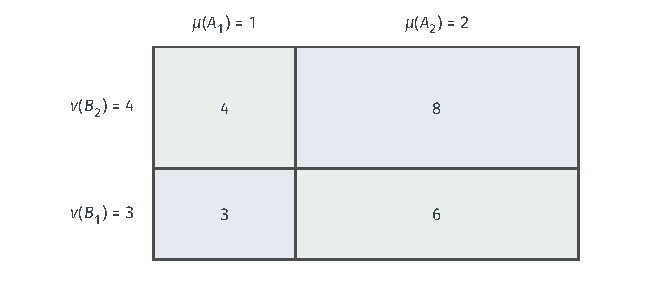
\includegraphics[width=112mm]{figures/00-shared/mathematical-preliminaries-upper/00-shared/tikz/chapter3-concept-processes/product-measure-grid.pdf}
 \caption{两列的权重分别为$1,2$（图中记为$\mu(A_1),\mu(A_2)$），两行的权重分别为$3,4$（记为$\nu(B_1),\nu(B_2)$）。四个格子的乘积权重为$3,6,4,8$，总量$21=(1+2)(3+4)$。列宽与行高按各自权重成比例，因此格子面积也按乘积成比例。这只是乘积赋权的有限示例，并非任意二维分布都满足的关系。}
 \label{fig:analysis-process-product-measure-grid}
\end{figure}

\paragraph{乘积$\sigma$代数}

矩形适合规定基本赋值，但矩形的并或补一般不再是矩形，例如两个长方形拼成的L形区域就不是矩形，因此不能只把矩形本身当作全部可测集合。
设$A\in\mathcal B(\mathbb R^p)$、$B\in\mathcal B(\mathbb R^q)$，称$A\times B$为Borel矩形。
包含全部Borel矩形的最小$\sigma$代数称为乘积$\sigma$代数，记为$\mathcal B(\mathbb R^p)\otimes\mathcal B(\mathbb R^q)$。
它和直接在$\mathbb R^{p+q}$中由开盒生成的Borel范围是同一个集合族：
\begin{equation}
 \mathcal B(\mathbb R^p)\otimes\mathcal B(\mathbb R^q)=\mathcal B(\mathbb R^{p+q}).
 \label{eq:comb-borel-product-structure}
\end{equation}

先证右侧包含于左侧。$\mathbb R^{p+q}$中的每个开盒都是$\mathbb R^p$中一个开盒与$\mathbb R^q$中一个开盒的乘积，因而是Borel矩形；每个开集又是可数个开盒的并，所以全部开集都在左侧，左侧作为$\sigma$代数就包含它们生成的$\mathcal B(\mathbb R^{p+q})$。

再证左侧包含于右侧，只需说明每个Borel矩形都是$\mathbb R^{p+q}$中的Borel集合。
考虑所有满足$A\times\mathbb R^q\in\mathcal B(\mathbb R^{p+q})$的集合$A\subseteq\mathbb R^p$。
开盒$A$使$A\times\mathbb R^q$成为开集，所以开盒都满足要求；又因为$(\mathbb R^p\setminus A)\times\mathbb R^q$是$A\times\mathbb R^q$的补集、$\bigl(\bigcup_nA_n\bigr)\times\mathbb R^q=\bigcup_n(A_n\times\mathbb R^q)$，满足要求的集合对补集和可数并封闭。
这些集合因而构成一个包含开盒的$\sigma$代数，从而包含全部$\mathcal B(\mathbb R^p)$。
同理$\mathbb R^p\times B$对每个$B\in\mathcal B(\mathbb R^q)$都是Borel集合，于是
$A\times B=(A\times\mathbb R^q)\cap(\mathbb R^p\times B)$属于$\mathcal B(\mathbb R^{p+q})$。
左侧的生成集合都在右侧，所以左侧包含于右侧。

\paragraph{乘积测度}

有了可测范围，还要为其中每个集合赋予联合的大小。对Borel矩形，所需规则就是把两个方向的测度相乘。

\begin{definition}[乘积测度]
\label{def:analysis-product-measure}
设$p,q\geq1$。在$\mathcal B(\mathbb R^p)\otimes\mathcal B(\mathbb R^q)$上，若一个测度对所有$A\in\mathcal B(\mathbb R^p)$、$B\in\mathcal B(\mathbb R^q)$满足
\begin{equation}
 (m_p\otimes m_q)(A\times B)=m_p(A)m_q(B),
 \label{eq:comb-product-measure-rectangle}
\end{equation}
就称它为$m_p$与$m_q$的\term{乘积测度}（product measure），记为$m_p\otimes m_q$，其中约定$0\cdot\infty=0$。
\end{definition}

约定$0\cdot\infty=0$有直观依据：平面上的直线$\mathbb R\times\{0\}$在横向长度无穷、纵向长度为零，它应当没有面积。
定义只规定了矩形应有的测度，还要确认这个规定能够一致地扩展到整个乘积$\sigma$代数，并且扩展只有一种。

\begin{theorem}[乘积测度的存在唯一性]
在$\mathcal B(\mathbb R^p)\otimes\mathcal B(\mathbb R^q)$上恰有一个测度满足式~\eqref{eq:comb-product-measure-rectangle}，它就是$m_{p+q}$在$\mathcal B(\mathbb R^{p+q})$上的限制。
\end{theorem}

存在性由$m_{p+q}$本身提供：对坐标盒，矩形规则就是体积的定义；从盒推进到一般Borel矩形，要利用两侧Borel集合都能被可数个盒从外侧逼近，这一步引用测度论教材\scite{math-folland1999real}。
唯一性的论证依赖两点：两个矩形的交仍是矩形；$\mathbb R^{p+q}$能被可数个有限体积的盒$(-n,n)^{p+q}$逐步填满。
两个测度若在全部矩形上取值相同，先在每个有限体积的盒内比较，再令$n\to\infty$，就能推出它们在整个乘积$\sigma$代数上相同，完整论证见同一教材。
两个一般测度空间也可以按同样的矩形规则作乘积，那时“能被可数个有限测度部分填满”成为必须单独检查的条件；其一般构造与条件已在本章前面的乘积测度中说明。

\paragraph{欧氏乘积与完备化}

上面的乘积测度只定义在Borel范围上，而区域积分使用的是更大的勒贝格范围$\mathcal L(\mathbb R^{p+q})$。
两者之间相差的只是零测集的子集：每个勒贝格可测集都能写成一个Borel集合与某个Borel零测集的子集之并\scite{math-folland1999real}。
把这些零测集的子集也补进可测范围，称为完备化；$m_{p+q}$在$\mathcal L(\mathbb R^{p+q})$上正是$m_p\otimes m_q$的完备化。

完备化不能靠先把两个因子完备化来代替：即使两个因子都取完备的勒贝格测度，它们的乘积$\sigma$代数也未必完备。
\begin{example}[勒贝格因子的乘积$\sigma$代数不完备]
\label{ex:region-product-sigma-algebra-incomplete}
取$p=q=1$，考虑由全部乘积$A\times B$（$A,B\in\mathcal L(\mathbb R)$）生成的乘积$\sigma$代数$\mathcal L(\mathbb R)\otimes\mathcal L(\mathbb R)$。

先说明其中每个集合$E$在每个$x$处的截面$E_x=\{y:(x,y)\in E\}$都勒贝格可测。
截面都可测的集合组成的族包含全部乘积$A\times B$，因为$(A\times B)_x$是$B$或$\varnothing$。取截面与取补集、可数并可以交换次序：$(\mathbb R^2\setminus E)_x=\mathbb R\setminus E_x$，$\bigl(\bigcup_nE_n\bigr)_x=\bigcup_n(E_n)_x$；所以这个族是$\sigma$代数，从而包含整个乘积$\sigma$代数。

再取一个勒贝格不可测集$S\subseteq\mathbb R$，令$E=\{0\}\times S$。
$E$包含在直线$\{0\}\times\mathbb R$中。这条直线是乘积$\{0\}\times\mathbb R$，乘积测度给它的值为$m(\{0\})m(\mathbb R)=0\cdot\infty=0$，所以$E$是乘积测度下零测集的子集；在完备的勒贝格范围$\mathcal L(\mathbb R^2)$中，$E$可测且零测。
但$E$在$x=0$处的截面是不可测集$S$，所以$E$不属于乘积$\sigma$代数。
\end{example}

因此下面陈述累次积分时，要分清函数对Borel范围可测，还是只对勒贝格范围可测；后者的结论需要附加“几乎处处”。

\subsection{区域积分的定义与可积性}
\label{sec:multivariable-riemann-lebesgue}

测度确定区域有多大，被积函数确定各位置贡献多少。
现在把一元可测函数与勒贝格积分的定义搬到$\mathbb R^d$上：改变的是输入空间和所用的测度，积分的构造步骤不变。

\subsubsection{多元可测函数}

累计函数值时，要把输入按函数值分层，例如取值在$[u,v)$之间的位置组成一层，这一层的贡献约为函数值乘该层的体积。
只有每一层都能测量，这种累计才有意义。
与一元情形一样，只需检查所有阈值集合$\{f>a\}$，因为$\{f\geq u\}=\bigcap_n\{f>u-1/n\}$、$\{u\leq f<v\}=\{f\geq u\}\setminus\{f\geq v\}$等集合都能由阈值集合经可数次集合运算得到。
\begin{definition}[多元可测函数]
设$D\in\mathcal L(\mathbb R^d)$。函数$f:D\to\overline{\mathbb R}$称为勒贝格可测函数，是指对每个$a\in\mathbb R$，集合
\[
 \{\bm x\in D:f(\bm x)>a\}
\]
都属于$\mathcal L(\mathbb R^d)$。若这些集合都属于$\mathcal B(\mathbb R^d)$，则称$f$为Borel可测函数。
\end{definition}

连续函数都可测：若$f$在$D$上连续，阈值集合$\{f>a\}$是开区间$(a,\infty)$的原像，因而相对于$D$开，可写为$D$与某个欧氏开集之交；$D$与开集都可测，所以阈值集合可测。
连续性只是可测性的充分条件：$\mathbb I_{\mathbb Q^d}$处处不连续，却是可测函数，因为它的阈值集合在$a<0$、$0\leq a<1$、$a\geq1$时分别是全空间、$\mathbb Q^d$和$\varnothing$，而可数集$\mathbb Q^d$零测，因而可测。

关于和、积、绝对值、最大最小值以及逐点极限保持可测性的论证只用到阈值集合的可数运算，在$\mathbb R^d$上照样成立。
例如分段给出的函数$f=g\mathbb I_{D_1}+h\mathbb I_{D_2}$，只要$g,h$在$\mathbb R^d$上连续、$D_1,D_2$可测，就是可测函数。
向量值函数的积分按分量进行，每个分量都是本节讨论的标量函数；例如质心的每个坐标都是一个标量区域积分与总质量之比。

\subsubsection{区域积分的定义}

\paragraph{非负标量函数的积分}

先累计非负贡献，就不会遇到正负无穷相消。
可测简单函数在每个可测小块上取常值，其积分等于各块的常值乘该块测度再求和；一般非负函数仍由下方的简单函数逼近。
\begin{definition}[区域上非负可测函数的积分]
设$D\in\mathcal L(\mathbb R^d)$，$f:D\to[0,\infty]$可测。定义
\[
 \int_D f\,\mathrm dm_d
 =\sup_{\substack{0\leq s\leq f\\s\text{为可测简单函数}}}
 \int_D s\,\mathrm dm_d.
\]
若$s=\sum_{j=1}^n c_j\mathbb I_{E_j}$，其中$E_j\subseteq D$可测、两两不交且$c_j\geq0$，则$\int_Ds\,\mathrm dm_d=\sum_jc_jm_d(E_j)$，约定$0\cdot\infty=0$。
\end{definition}

把$f$看成薄片的面密度，就能读出这个定义的含义。
满足$0\leq s\leq f$的简单函数把区域分成有限块，并在每块上用一个不超过真实密度的常数代替密度，所以$\int_Ds$是总质量的一个偏小估计；对所有这样的估计取上确界，就得到总质量。

也可以从体积来读：$c_j\mathbb I_{E_j}$对应以$E_j$为底、高为$c_j$的柱体$E_j\times[0,c_j)$，由乘积测度的矩形规则，它的$(d+1)$维体积就是$c_jm_d(E_j)$。
于是$\int_Ds$是排在$f$的图像下方的一组柱体的总体积，上确界则是图像下方整个区域的体积；第~\ref{sec:multivariable-iterated-integrals}节会用Tonelli定理把这个读法写成等式。

这个积分可以取$+\infty$，例如$f\equiv1$在整个平面上的积分是平面的面积$+\infty$。
在全空间上把$f$作零延拓，就有
$\int_Df\,\mathrm dm_d=\int_{\mathbb R^d}f\mathbb I_D\,\mathrm dm_d$，其中$f\mathbb I_D$在$D$内等于$f$、在$D$外取零；以后在区域上积分，都可以看成对零延拓后的函数在全空间上积分。
区域不必是矩形，定义也不要求它的边界零测；这与黎曼积分先用矩形网格逼近区域的做法不同。

\paragraph{有符号标量函数的积分}

函数可以取正负值时，例如带电薄片上既有正电荷也有负电荷，应先分别累计正负贡献：$f^+=\max\{f,0\}$给出正电荷的密度，$f^-=\max\{-f,0\}$给出负电荷的密度，净电荷是两者总量之差。
与一元情形相同，为了让这个差是一个普通的有限数，要求绝对值的总贡献有限。
\begin{definition}[区域上可测函数的积分]
设$D\in\mathcal L(\mathbb R^d)$，$f:D\to\overline{\mathbb R}$可测。若
\begin{equation}
 \int_D|f|\,\mathrm dm_d<\infty,
 \label{eq:multivariable-lebesgue-integrability}
\end{equation}
称$f$在$D$上勒贝格可积，并定义
\[
 \int_Df\,\mathrm dm_d=\int_Df^+\,\mathrm dm_d-\int_Df^-\,\mathrm dm_d.
\]
\end{definition}

由于$|f|=f^++f^-$，条件~\eqref{eq:multivariable-lebesgue-integrability}同时保证正负两部分的积分都有限，相减不会出现$\infty-\infty$。
这个条件不成立时，至少有一部分积分为无穷；若两部分都为无穷，两者之差没有意义，也就不能用相减定义勒贝格积分。

条件~\eqref{eq:multivariable-lebesgue-integrability}还保证$f$几乎处处取有限值。
集合$N=\{|f|=\infty\}$对每个$M>0$满足$M\mathbb I_N\leq|f|$，所以$Mm_d(N)\leq\int_D|f|$对所有$M$成立，只能$m_d(N)=0$；在$N$上把无穷值改成零，不改变积分。

与黎曼积分相比，这一定义不要求函数在细小的网格块上接近常数。
例如$\mathbb I_{\mathbb Q^d}$在单位立方体上不黎曼可积：每个小盒中都既有有理点又有无理点，上和恒为$1$而下和恒为$0$；但它的勒贝格积分为零，因为可数集的$d$维测度为零。

\paragraph{Riemann积分与勒贝格积分的一致性}
现在可以比较前面定义的经典积分与这里的勒贝格积分。两种理论在共同范围内一致：若有界函数$g$在闭盒上Riemann可积，则它勒贝格可积，两种积分相等。先取一列逐次加细的网格，使网格趋细且上下和之差趋于零。按半开小盒约定，相应下、上阶梯函数逐点夹住$g$，两者分别递增和递减，差的勒贝格积分趋于零。差的逐点极限非零的点组成零测集：对任意$\eta>0$，差的极限不小于$\eta$的集合，其测度不超过每一级差的积分除以$\eta$，因此为零。零测集之外，上下阶梯函数收敛到同一个值，而被夹住的$g$也等于这个值；在零测集内的值由勒贝格测度的完备性处理，于是$g$可测。

上下阶梯函数的勒贝格积分正是下、上和。上下和之差趋于零，故被夹在中间的勒贝格积分只能等于Riemann极限。对Jordan区域上的零延拓也同样成立。反过来，勒贝格可积并不保证Riemann可积，前述$\mathbb I_{\mathbb Q^2}$在盒上的勒贝格积分为零，就是一个区别。

\paragraph{二重积分与多重积分}

二维时把上述积分写为
\[
 \iint_Df(x,y)\,\mathrm dx\,\mathrm dy=\int_Df\,\mathrm dm_2;
\]
三维中常记为$\iiint_Df\,\mathrm dV$；$d$维时统一写作
\[
 \int_Df(\bm x)\,\mathrm d\bm x=\int_Df\,\mathrm dm_d.
\]
“二重”或“多重”表示输入维数，并不表示已经选择了逐坐标的计算次序。
例如$f\equiv3$、$D=[0,1]\times[0,2]$时，积分为$3m_2(D)=6$：密度处处为$3$、面积为$2$的薄片，总质量为$6$。

当$0<m_d(D)<\infty$且$f$可积时，
\[
 \frac{1}{m_d(D)}\int_Df\,\mathrm dm_d
\]
称为$f$在$D$上的平均值。
它是一个常数，用它代替$f$铺满整个$D$，总累计不变。上例的平均值为$3$。

\subsubsection{可积性的判别}

按定义，可测函数$f$在$D$上可积，意思是非负积分$\int_D|f|\,\mathrm dm_d$有限。
这个非负积分总有定义，只是可能等于$+\infty$；判别可积性因此只需回答一个问题：$|f|$在$D$上的总累计是有限还是无穷。
直接从上确界定义计算这个量往往不现实，下面三种做法都用更容易得到的量来估计它：用函数的上界乘区域的测度；用一列测度有限的递增子区域逼近$D$，看这些子区域上的累计是否有共同上界；与一个已知是否可积的函数逐点比较。

若$f$有界且$D$的测度有限，第一种做法立即给出有限上界。
由此可见，累计变为无穷只能是因为$f$无界（例如在某些位置附近无界），或者$D$的测度无穷；后两种做法正是为这两种情形准备的。

\paragraph{有界函数且有界区域}

设区域$D$有界，从而$m_d(D)<\infty$（更一般地，只要$m_d(D)<\infty$即可），$f$可测且$|f|\leq M<\infty$几乎处处成立。
这时$|f|\leq M\mathbb I_D$几乎处处成立，由非负积分的单调性，
\[
 \int_D|f|\,\mathrm dm_d\leq M m_d(D)<\infty.
\]
物理上，总质量不超过最大密度乘面积。
由有限维闭有界集上连续函数的有界性，闭有界集上的连续函数有界，所以闭有界区域上的连续函数可积。

这一判别只用到有界性，不要求函数能连续地延伸到区域的边界。
\begin{example}[开正方形上剧烈振荡的有界函数可积]
\label{ex:region-bounded-oscillation}
在开正方形$(0,1)^2$上令$f(x,y)=\sin\bigl(1/(xy)\bigr)$。
$f$在开正方形上连续，因而可测。
它不能连续延拓到闭正方形：固定$x=t\in(0,1)$，令$y\downarrow0$，则$1/(ty)\to+\infty$，$f(t,y)$在$-1$与$1$之间无穷次振荡，没有极限。
所以闭有界集上的极值定理不能直接使用。
但$|f|\leq1$且$m_2\bigl((0,1)^2\bigr)=1$，由上面的估计，
\[
 \int_{(0,1)^2}|f|\,\mathrm dm_2\leq1,
\]
所以$f$在$(0,1)^2$上可积。
\end{example}

这个判别不适用于两类情形：函数无界，或区域的测度无穷。
在这两类情形中，可积与不可积都可能发生。
无界函数仍可能可积，示例~\ref{ex:region-power-function-threshold}将说明$\lVert\bm x\rVert_2^{-1}$在平面单位圆盘上可积；无限测度区域上的有界函数则未必可积，例如$f\equiv1$在整个平面上积分为无穷。
判断这两类情形需要更细的估计。

\paragraph{无界函数或无限区域}

处理无界函数或无限区域时，可以先避开麻烦的位置。
取一列递增的可测集合$D_1\subseteq D_2\subseteq\cdots$，使$\bigcup_nD_n=D$，并让每个$D_n$避开函数无界的位置、只占有限测度；例如函数只在原点附近无界时，可取$D_n=D\cap\{1/n\leq\lVert\bm x\rVert_2\leq n\}$。
这时每个$\int_{D_n}|f|$通常可以用有界函数在有限测度区域上的估计确认有限。
由于$0\leq|f|\mathbb I_{D_n}\uparrow|f|\mathbb I_D$，单调收敛定理给出
\[
 \int_D|f|\,\mathrm dm_d
 =\lim_{n\to\infty}\int_{D_n}|f|\,\mathrm dm_d
 =\sup_n\int_{D_n}|f|\,\mathrm dm_d.
\]
因此$f$在$D$上可积，当且仅当截断累计$\int_{D_n}|f|$有一个与$n$无关的有限上界。
这说明递增截断下的非负积分有界，当且仅当整个区域上的非负积分有限；这一论证只用单调收敛，不依赖维数。
只知道每个截断累计分别有限还不够，必须检查它们是否共同有界。

截断累计也可以改写成级数。
把区域拆成两两不交的“壳层”$A_k=D_k\setminus D_{k-1}$（$D_0=\varnothing$），由积分的区域可加性，
$\int_D|f|=\sum_k\int_{A_k}|f|$，可积性就化为一个非负级数是否收敛。

只依赖半径的函数适合用壳层估计。
下面按半径成倍增长划分壳层，判别平面幂函数在原点附近和远处的可积性。
\begin{example}[平面幂函数$\lVert\bm x\rVert_2^{-p}$的可积阈值]
\label{ex:region-power-function-threshold}
设$p>0$，$f(\bm x)=\lVert\bm x\rVert_2^{-p}$，$\bm x\in\mathbb R^2\setminus\{\bm 0\}$。按半径成倍增长的圆环
\[
 A_k=\{\bm x\in\mathbb R^2:2^k\leq\lVert\bm x\rVert_2<2^{k+1}\},\qquad k\in\mathbb Z
\]
把$\mathbb R^2\setminus\{\bm 0\}$分成两两不交的壳层。

记$\alpha=m_2(A_0)$。它是一个有限正数：$A_0$含有小盒，又含于盒$(-2,2)^2$。
由伸缩性质，$A_k=2^kA_0$，所以$m_2(A_k)=4^k\alpha$。
在$A_k$上$2^{-(k+1)p}<\lVert\bm x\rVert_2^{-p}\leq2^{-kp}$，乘以$m_2(A_k)$得到
\[
 2^{-p}\alpha\,2^{k(2-p)}\leq\int_{A_k}\lVert\bm x\rVert_2^{-p}\,\mathrm d\bm x\leq\alpha\,2^{k(2-p)}.
\]

单位圆外由$k=0,1,2,\ldots$的壳层组成，各壳层的贡献与公比为$2^{2-p}$的几何级数同阶，累计有限当且仅当$p>2$。
单位圆内（去掉原点）由$k=-1,-2,\ldots$的壳层组成；令$j=-k$，各壳层的贡献与$2^{j(p-2)}$同阶，累计有限当且仅当$p<2$。
因此$\lVert\bm x\rVert_2^{-p}$在单位圆盘上可积当且仅当$p<2$，在单位圆外可积当且仅当$p>2$；$p=2$时两侧都不可积，在整个平面上则对任何$p>0$都不可积。
\end{example}

在$\mathbb R^d$中把面积因子$4^k$换成$2^{kd}$，同样的计算给出阈值$d$；$d=1$时恢复一元幂函数积分的阈值$1$。
这个阈值比较的是两种速度：靠近原点时，函数按$r^{-p}$增大，而半径约为$r$的壳层的体积按$r^d$缩小；远离原点时，函数按$r^{-p}$减小，壳层的体积按$r^d$增大。
第~\ref{sec:multivariable-change-variables}节将用极坐标直接计算圆环上的积分，验证这里的结论（示例~\ref{ex:region-polar-power-check}）。

确认可积以后，截断积分还能用来计算有符号积分。
由$|f\mathbb I_{D_n}|\leq|f|$，支配收敛定理给出$\int_{D_n}f\to\int_Df$，误差不超过$\int_{D\setminus D_n}|f|$，所以无论选哪一列递增区域，都得到同一个值。

缺少绝对可积性时，截断极限可能依赖区域的选法。
\begin{example}[截断极限依赖截断方式]
\label{ex:region-truncation-dependence}
在平面上令$f(x,y)=1$（$x>0$），$f(x,y)=-1$（$x\leq0$）。
取正方形$D_n=(-n,n)^2$时，右半部分与左半部分的面积都是$2n^2$，正负贡献恰好抵消，每个$\int_{D_n}f=0$。
取偏向右侧的长方形$D_n'=(-n,2n)\times(-n,n)$时，右侧部分面积为$4n^2$，左侧部分面积为$2n^2$，所以$\int_{D_n'}f=2n^2\to+\infty$。
两列截断都递增地填满整个平面，极限却分别是$0$和$+\infty$。
\end{example}

例中$\int|f|=+\infty$，两种截断的不同极限都不能当作$f$的积分。
截断只能用来计算已经确认绝对可积的函数的积分。

\paragraph{比较判别：可积上界与不可积下界}

有了一族可积性已知的函数，就可以把新函数与它们逐点比较，而不必每次重新做壳层计算。
比较有两个方向，都来自非负积分的单调性：
\begin{itemize}
 \item 若存在非负可积函数$H$，使$|f|\leq H$在$D$上几乎处处成立，则$\int_D|f|\leq\int_DH<\infty$，$f$可积；
 \item 若存在非负可测函数$g$，使$|f|\geq g$在$D$上几乎处处成立且$\int_Dg=+\infty$，则$\int_D|f|=+\infty$，$f$不可积。
\end{itemize}
比较只需在可能出问题的位置进行：先用区域可加性把$D$拆成函数有界且测度有限的部分和“原点附近”“远处”等部分，前者用有界判别，其余部分再与幂函数比较。

远处的比较看函数衰减得有多快。
\begin{example}[远处与$r^{-3}$和$r^{-2}$比较]
\label{ex:region-comparison-at-infinity}
记$r=\lVert\bm x\rVert_2$，其中$\bm x=(x,y)$。

函数$f(x,y)=\cos(xy)/(1+x^2+y^2)^{3/2}$在整个平面上可积。
在单位圆盘内$|f|\leq1$，用有界判别；在单位圆外$|f|\leq(1+r^2)^{-3/2}\leq r^{-3}$，而由示例~\ref{ex:region-power-function-threshold}，$p=3>2$的幂函数在圆外可积。

函数$g(x,y)=1/(1+x^2+y^2)$在整个平面上不可积。
在单位圆外$1+r^2\leq2r^2$，所以$g\geq r^{-2}/2$，而$p=2$的幂函数在圆外累计无穷。
\end{example}

一元的$1/(1+x^2)$在实轴上可积，二元的类似函数却不可积。
原因在于远处可用的范围增长得更快：半径为$R$的圆盘面积按$R^2$增长，而区间$[-R,R]$的长度只按$R$增长。

原点附近的比较同样只看奇点处的增长速度。
\begin{example}[原点附近的对数奇点与平方倒数奇点]
\label{ex:region-comparison-near-origin}
仍记$r=\lVert\bm x\rVert_2$，在单位圆盘$\{r\leq1\}$上考察两个在原点附近无界的函数。

$\log(x^2+y^2)=2\log r$在$r\downarrow0$时趋于$-\infty$。
函数$t\mapsto t|\log t|$在$(0,1)$上的最大值为$1/e$，在$t=1/e$处取到，所以$0<r<1$时
\[
 |\log r^2|=2|\log r|\leq\frac2e\,r^{-1}.
\]
与$p=1<2$的幂函数比较，可知$\log(x^2+y^2)$在单位圆盘上可积。

$(x^2+2y^2)^{-1}$满足$x^2+2y^2\leq2(x^2+y^2)=2r^2$，所以$(x^2+2y^2)^{-1}\geq r^{-2}/2$。
与$p=2$的幂函数比较，可知它在单位圆盘上不可积。
\end{example}

找不到合适的比较函数时，还可以用第~\ref{sec:multivariable-iterated-integrals}节的Tonelli定理把$\int_D|f|$化为累次积分直接计算，再判断它是否有限。

\subsection{区域积分的基本性质}

多维区域积分仍由非负简单函数逼近构造，只是测度使用$m_d$。
一般测度空间上的单调收敛定理、Fatou引理、支配收敛定理以及下面各条积分性质，证明都只用到简单函数逼近、测度的可数可加性和这些结论之间的推导，不依赖输入只有一个坐标，因此在$\mathbb R^d$上可以直接使用。
下面固定可测区域$D$，各有符号公式均要求所列函数在相应区域上绝对可积，微元统一写为$\mathrm dm_d$。

\paragraph{加法}

若$f,g$在$D$上可积，则$f+g$也可积，且
\[
 \int_D(f+g)\,\mathrm dm_d=\int_Df\,\mathrm dm_d+\int_Dg\,\mathrm dm_d.
\]
绝对可积性由$|f+g|\leq|f|+|g|$保证，相加公式由一般勒贝格积分的线性给出。
物理上，两种物质叠放在同一块薄片上时，总质量等于两种物质的质量之和。

\paragraph{减法}

若$f,g$在$D$上可积，则
\[
 \int_D(f-g)\,\mathrm dm_d=\int_Df\,\mathrm dm_d-\int_Dg\,\mathrm dm_d.
\]
这里两项都是有限数，因此不会出现无穷减无穷。

\paragraph{数乘}

若$c\in\mathbb R$且$f$在$D$上可积，则$cf$可积，并满足
\[
 \int_Dcf\,\mathrm dm_d=c\int_Df\,\mathrm dm_d.
\]
系数只改变各位置的标量贡献，不改变积分区域及其测度；例如把密度的单位从千克换成克，总质量的数值同样乘$1000$。

\paragraph{区域可加性}

若$f$在有限个或可数个两两不交的可测集合$D_j$之并上可积，则
\[
 \int_{\bigcup_jD_j}f\,\mathrm dm_d=\sum_j\int_{D_j}f\,\mathrm dm_d.
\]
也就是说，把一块区域分成若干块分别累计再相加，与整体累计相同。
有限并直接来自指示函数的分解，可数并使用一般积分的区域可加性；绝对可积性保证右侧级数绝对收敛。

两块区域允许重叠时，只需扣除被重复计入的交集：
\[
 \int_{A\cup B}f\,\mathrm dm_d
 =\int_Af\,\mathrm dm_d+\int_Bf\,\mathrm dm_d-\int_{A\cap B}f\,\mathrm dm_d.
\]
这由$\mathbb I_{A\cup B}=\mathbb I_A+\mathbb I_B-\mathbb I_{A\cap B}$得到。
若沿连续函数的图像这类曲线或曲面把区域切成几块，公共边界是零测集（第~\ref{sec:multivariable-iterated-integrals}节用Tonelli定理证明这一点），重叠部分不影响积分，因此可以直接把各块的积分相加。

\paragraph{单调性}

若$f,g$在$D$上可积且$f\leq g$几乎处处成立，则
\[
 \int_Df\,\mathrm dm_d\leq\int_Dg\,\mathrm dm_d.
\]
特别地，$a\leq f\leq b$几乎处处成立且$0<m_d(D)<\infty$时，有$a\,m_d(D)\leq\int_Df\leq b\,m_d(D)$，即平均值落在$[a,b]$内。
同一估计也给出忽略一小块区域$E$时的误差上界：若在$E$上$|f|\leq M$，则舍去$E$造成的误差$\bigl|\int_Ef\bigr|$不超过$Mm_d(E)$。

\paragraph{绝对值不等式}

可积函数满足
\[
 \left|\int_Df\,\mathrm dm_d\right|\leq\int_D|f|\,\mathrm dm_d.
\]
它来自$-|f|\leq f\leq|f|$和积分单调性。左侧允许正负贡献相消，右侧不允许，因此净量的大小不超过总量。

由于零测集贡献为零，上述所有性质都允许在零测集上修改有限函数值；测度的完备性保证这种修改保持可测。

\subsection{累次积分}
\label{sec:multivariable-iterated-integrals}

直接从定义计算区域积分往往不现实。
求一块面包的体积时，可以先把它切成平行的薄片，每片的体积约为截面面积乘片厚，再把所有薄片的体积相加。
同样，求薄片的总质量时，可以先沿每一条竖线累计质量，得到这条竖线上的“线密度”，再沿横向累计各条竖线的贡献。
这种“先在每个截面上累计，再累计截面”的计算称为累次积分，它把一次$d$维累计化成几次低维累计。
累次积分是否等于区域积分，要检查非负性或绝对可积性；交换累计次序也不只是调换微分记号的位置。

\subsubsection{截面与累次积分}

把$\mathbb R^d$写成$\mathbb R^p\times\mathbb R^q$，点写成$(\bm x,\bm y)$，其中$\bm x\in\mathbb R^p$、$\bm y\in\mathbb R^q$；最常见的是$p=q=1$。
对$f:\mathbb R^p\times\mathbb R^q\to\overline{\mathbb R}$，固定$\bm x$所得的函数$f_{\bm x}(\bm y)=f(\bm x,\bm y)$称为关于$\bm y$的截面。
区域$D$上的函数先作零延拓，截面就在$D$的截面$D_{\bm x}=\{\bm y:(\bm x,\bm y)\in D\}$以外取零；例如单位圆盘在$x\in[-1,1]$处的截面是区间$[-\sqrt{1-x^2},\sqrt{1-x^2}]$。

若各截面的积分有意义，所得关于$\bm x$的函数的积分也有意义，则
\[
 \int_{\mathbb R^p}\left(\int_{\mathbb R^q}f(\bm x,\bm y)\,\mathrm d\bm y\right)\mathrm d\bm x
\]
称为先对$\bm y$、再对$\bm x$的累次积分。
内层积分把$\bm x$视为固定的数，算出截面$D_{\bm x}$上的总量；外层积分再把这些截面总量按$\bm x$累计。
交换两组变量的角色，就得到先对$\bm x$、再对$\bm y$的累次积分。
两种次序是否相等，以及它们是否等于区域积分，不能由记号推出，要由下面的定理判断。

有限网格上的这种计算就是先求每行的加权和，再把各行的结果相加；示例~\ref{ex:region-finite-product-weights}和图~\ref{fig:analysis-process-product-measure-grid}中两种次序都得到$21$。
那里的联合权重是两侧权重之积；二元概率分布何时能写成两个边缘分布的乘积，即独立性问题，可参考\BookChapterRef{chap:probability-theory}{卷2《数学准备：概率、因果与决策》的“随机变量与概率基础”章}。

\subsubsection{累次积分的成立条件}

下面先对Borel可测函数陈述结论，这时每个截面都Borel可测。
若函数只对勒贝格范围$\mathcal L(\mathbb R^{p+q})$可测，就可能出现示例~\ref{ex:region-product-sigma-algebra-incomplete}中的现象：该例中集合$E$的指示函数勒贝格可测，却在零面积的直线$x=0$上取不可测的截面。
因此对勒贝格可测函数，截面的可测性和内层积分都只对几乎每个坐标成立。

\paragraph{非负可测函数的累次积分}

非负贡献不会因相消而改变总量，因此允许总积分为无穷。
Tonelli定理说明，对非负函数，两种次序的累次积分都等于区域积分。
\begin{theorem}[Tonelli定理]
\label{thm:analysis-tonelli-fubini}
设$p,q\geq1$，$f:\mathbb R^p\times\mathbb R^q\to[0,\infty]$为Borel可测函数。则每个截面$\bm y\mapsto f(\bm x,\bm y)$与$\bm x\mapsto f(\bm x,\bm y)$都Borel可测，两个内层积分函数
\[
 \bm x\longmapsto\int_{\mathbb R^q}f(\bm x,\bm y)\,\mathrm d\bm y,\qquad
 \bm y\longmapsto\int_{\mathbb R^p}f(\bm x,\bm y)\,\mathrm d\bm x
\]
也分别Borel可测，且
\[
 \begin{aligned}
 \int_{\mathbb R^{p+q}}f\,\mathrm dm_{p+q}
 &=\int_{\mathbb R^p}\left(\int_{\mathbb R^q}f(\bm x,\bm y)\,\mathrm d\bm y\right)\mathrm d\bm x\\
 &=\int_{\mathbb R^q}\left(\int_{\mathbb R^p}f(\bm x,\bm y)\,\mathrm d\bm x\right)\mathrm d\bm y.
 \end{aligned}
\]
三个积分允许共同取$+\infty$。若$f$只是勒贝格可测，上述等式仍成立，但截面只对几乎每个$\bm x$（相应地，几乎每个$\bm y$）勒贝格可测，内层积分函数只在几乎处处有定义，且是勒贝格可测函数。
\end{theorem}

\paragraph{绝对可积函数的累次积分}

有符号函数不能只依靠逐行或逐列的有限值来保证换序。
先对$|f|$应用非负版本，确认整个区域上的绝对贡献有限，就能排除正负无穷相消。
\begin{theorem}[Fubini定理]
\label{thm:analysis-fubini-integrable}
设$f:\mathbb R^p\times\mathbb R^q\to\overline{\mathbb R}$勒贝格可测，并满足
$\int_{\mathbb R^{p+q}}|f|\,\mathrm dm_{p+q}<\infty$。
则截面$f_{\bm x}$对几乎每个$\bm x$可积，另一方向的截面也对几乎每个$\bm y$可积。
把内层积分函数在相应例外集上置为零后，它们分别可积，并且
\[
 \begin{aligned}
 \int_{\mathbb R^{p+q}}f\,\mathrm dm_{p+q}
 &=\int_{\mathbb R^p}\left(\int_{\mathbb R^q}f(\bm x,\bm y)\,\mathrm d\bm y\right)\mathrm d\bm x\\
 &=\int_{\mathbb R^q}\left(\int_{\mathbb R^p}f(\bm x,\bm y)\,\mathrm d\bm x\right)\mathrm d\bm y.
 \end{aligned}
\]
三个积分都是有限值。若$f$是Borel可测函数，例外集以外的截面也都是Borel可测函数。
\end{theorem}

若$f$在零测集上取无穷值，可先把那些值改成零再处理有符号积分；定义有符号积分时已经说明，绝对积分有限时这个集合零测，改值不影响积分。

两个定理的证明可分为集合与函数两层，这里只给出依赖路线，不把矩形上的核对当作完整证明。
集合层从矩形出发。
对矩形指示函数$\mathbb I_{A\times B}$，固定$\bm x$后的内层积分是$\mathbb I_A(\bm x)m_q(B)$，外层积分是$m_p(A)m_q(B)$，由乘积测度的矩形规则，它也等于$m_{p+q}(A\times B)$；有限可加性把这个结论推广到有限个不交矩形之并。
从这些集合推进到乘积$\sigma$代数中的任意Borel集合，需要测度论的扩张论证，不是仅靠每个矩形上的等式便能完成，完整论证见\scite{math-folland1999real}。

函数层沿用积分的构造步骤。
集合层的结论就是指示函数的结论，经线性组合推广到非负简单函数，再取简单函数列$s_n\uparrow f$，由单调收敛推广到任意非负Borel可测函数，得到Tonelli定理。
对勒贝格可测函数，先找一个与它几乎处处相等的Borel可测函数，二者的差异包含在一个Borel零测集$N$中；对$\mathbb I_N$用Tonelli定理得$\int m_q(N_{\bm x})\,\mathrm d\bm x=m_{p+q}(N)=0$，所以几乎每个截面$N_{\bm x}$零测，修改不影响内层积分。
若$f$绝对可积，则对$f^+$和$f^-$分别应用Tonelli定理；绝对积分有限保证两部分不会出现无穷减无穷，相减即得Fubini定理。
对两个更一般的测度作乘积时，Tonelli与Fubini定理在相应的有限覆盖条件下同样成立，前面的乘积测度已经给出了相应条件。

两个定理合起来给出一个实用的判别。
先对$|f|$应用Tonelli定理：只要任意一种次序的非负累次积分$\int\left(\int|f|\,\mathrm d\bm y\right)\mathrm d\bm x$有限，区域绝对积分就有限；随后才能对$f$使用Fubini定理，在两种次序之间自由切换。

Tonelli定理也把“积分等于图像下方的体积”写成了等式。
设$f:\mathbb R^d\to[0,\infty]$为Borel可测函数，令$\Gamma=\{(\bm x,t)\in\mathbb R^d\times\mathbb R:0\leq t<f(\bm x)\}$为图像下方的区域。
若$0\leq t<f(\bm x)$，就能取有理数$r$使$t<r<f(\bm x)$，所以
$\Gamma=\bigcup_{r\in\mathbb Q,\,r>0}\bigl(\{f>r\}\times[0,r)\bigr)$是可数个Borel矩形之并，是Borel集合。
对$\mathbb I_\Gamma$先沿$t$方向积分，固定$\bm x$时的截面是区间$[0,f(\bm x))$，长度为$f(\bm x)$，于是
\[
 m_{d+1}(\Gamma)=\int_{\mathbb R^d}\left(\int_{\mathbb R}\mathbb I_\Gamma(\bm x,t)\,\mathrm dt\right)\mathrm d\bm x=\int_{\mathbb R^d}f\,\mathrm dm_d.
\]

同样的截面论证说明图像本身没有体积。
设$f$是有限值Borel函数，它的图像$\{(\bm x,f(\bm x))\}$是Borel函数$(\bm x,t)\mapsto t-f(\bm x)$的零点集，因而是Borel集合；图像在每个$\bm x$处的截面只有一个点，长度为零，由Tonelli定理，图像是$(d+1)$维零测集。
例如圆周由上下两个半圆的图像组成，因此面积为零；把区域沿这类曲线切开时，边界确实不影响积分。

\subsubsection{累次积分的计算}

设$R=[a,b]\times[c,d]$，其中$a<b$、$c<d$，且$f$在$R$上连续。
连续函数在闭有界矩形上有界，因而在$R$上绝对可积，Fubini定理保证可以先按一个坐标累计、再按另一个坐标累计，且两种次序给出同一结果：
\[
 \begin{aligned}
 \int_R f(x,y)\,\mathrm d(x,y)
 &=\int_a^b\left(\int_c^d f(x,y)\,\mathrm dy\right)\mathrm dx\\
 &=\int_c^d\left(\int_a^b f(x,y)\,\mathrm dx\right)\mathrm dy.
 \end{aligned}
\]
左侧是一次区域累计，右侧两个累次积分是具体的逐次计算。这里的连续性也满足前面由Riemann和推出累次积分的条件；勒贝格框架给出了更一般的适用范围。

计算内层积分时，另一个坐标当作常数。
\begin{example}[矩形上$x+y$的两种累次积分]
\label{ex:region-rectangle-iterated}
令$f(x,y)=x+y$，$R=[0,1]\times[0,2]$，$f$在$R$上连续。先对$y$积分，
\[
 \int_0^1\left[xy+\frac{y^2}{2}\right]_{y=0}^{y=2}\,\mathrm dx
 =\int_0^1(2x+2)\,\mathrm dx=3.
\]
内层运算把$x$视为固定数，结果$2x+2$是竖线$\{x\}\times[0,2]$上的累计，再交给外层积分。
先对$x$积分，则
\[
 \int_0^2\left[\frac{x^2}{2}+xy\right]_{x=0}^{x=1}\,\mathrm dy
 =\int_0^2\left(\frac12+y\right)\mathrm dy=3,
\]
两种次序给出同一结果。区域面积为$2$，所以$f$在$R$上的平均值为$3/2$。
\end{example}

一般区域先作零延拓。
若区域写为$D=\{(x,y):a\leq x\leq b,\ \alpha(x)\leq y\leq\beta(x)\}$，其中上下边界$\alpha\leq\beta$在$[a,b]$上连续，则$D$是闭集，固定$x$的截面是区间$[\alpha(x),\beta(x)]$。
因此对$D$上非负可测或可积的$f$，以下等式成立；对一般勒贝格可测函数，内层截面积分按前述定理在几乎每个$x$处理解：
\[
 \iint_Df\,\mathrm dx\,\mathrm dy=\int_a^b\left(\int_{\alpha(x)}^{\beta(x)}f(x,y)\,\mathrm dy\right)\mathrm dx.
\]
内积分的上下限$\alpha(x),\beta(x)$正是截面的两个端点。改变积分次序时，应改为固定$y$、重新描述同一个区域的横截面。

同一个区域可以有两种截面描述，换序时两套上下限都要从区域本身读出。
\begin{example}[三角形区域上交换积分次序]
\label{ex:region-triangle-order-swap}
令$D=\{(x,y):0\leq y\leq x\leq1\}$，在$D$上累计常数$1$。
固定$x\in[0,1]$时，纵截面是$0\leq y\leq x$，先对$y$积分得到
\[
 \int_0^1\left(\int_0^x1\,\mathrm dy\right)\mathrm dx=\int_0^1x\,\mathrm dx=\frac12.
\]
固定$y\in[0,1]$时，同一区域的横截面是$y\leq x\leq1$，先对$x$积分得到
\[
 \int_0^1\left(\int_y^11\,\mathrm dx\right)\mathrm dy=\int_0^1(1-y)\,\mathrm dy=\frac12.
\]
两种次序都给出三角形的面积$1/2$。
\end{example}

若只交换微分记号而保留原来的上下限，所描述的就不再是同一个区域。
图~\ref{fig:analysis-process-region-slicing-orders}把这两种切片画在同一个区域上，突出换序时内层上下限也要改变。
\begin{figure*}[!htbp]
 \centering
 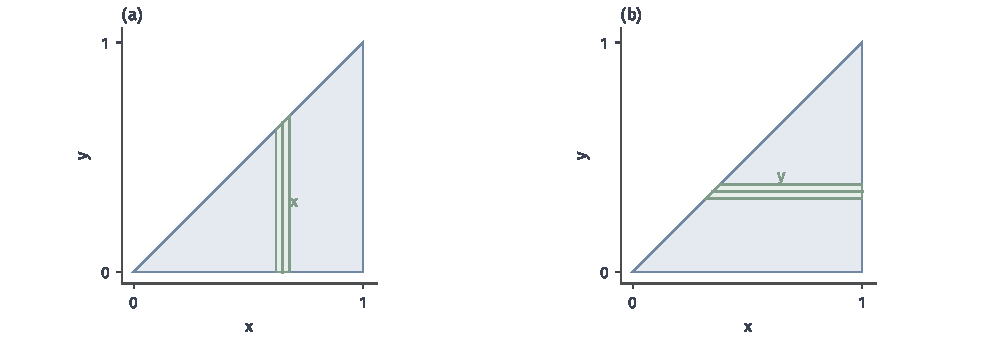
\includegraphics[width=169.0mm]{figures/00-shared/mathematical-preliminaries-upper/00-shared/matplotlib/chapter3-concept-processes/region-slicing-orders.pdf}
 \caption{$D=\{0\leq y\leq x\leq1\}$在两图完全相同。(a) 固定$x$，纵截面为$0\leq y\leq x$；(b) 固定$y$，横截面为$y\leq x\leq1$。绿色窄条仅示意一次切片，图中的条宽不充当实际微元。两种累计$1$都得面积$1/2$；换序依据非负性或绝对可积性，而非图形本身。}
 \label{fig:analysis-process-region-slicing-orders}
\end{figure*}

换序有时决定一个积分能否算出来。
\begin{example}[换序计算含$e^{y^2}$的累次积分]
\label{ex:region-exp-square-order-swap}
考虑
\[
 \int_0^1\left(\int_x^1e^{y^2}\,\mathrm dy\right)\mathrm dx.
\]
内层的$e^{y^2}$没有初等原函数，按原次序无法用原函数直接计算。
积分区域是闭三角形$\{(x,y):0\leq x\leq y\leq1\}$，被积函数在其上连续，因而绝对可积，可以交换次序。
固定$y\in[0,1]$时，横截面是$0\leq x\leq y$，于是
\[
 \int_0^1\left(\int_0^ye^{y^2}\,\mathrm dx\right)\mathrm dy
 =\int_0^1ye^{y^2}\,\mathrm dy
 =\frac{e-1}{2}.
\]
\end{example}

内层对$x$积分时$e^{y^2}$是常数，只产生截面长度$y$，而这个因子$y$恰好使外层积分有原函数$\frac12e^{y^2}$。

\subsubsection{积分换序的适用边界}

非负函数没有正负相消，累计可以为无穷；绝对可积函数允许取正负值，但正负两部分的累计各自有限。
两者都缺失时，两种累计次序可能以不同方式配对正负贡献，交换次序就可能改变结果，甚至一个次序收敛而另一个次序发散。

最直观的例子来自双重级数。
设$a_{i,j}$（$i,j\geq1$）是一个无穷矩阵，在第一象限上令
$f(x,y)=a_{i,j}$于$(x,y)\in[i-1,i)\times[j-1,j)$，即每个边长为$1$的方格上取对应的矩阵元素。
对$x\in[i-1,i)$，截面积分$\int_0^\infty f(x,y)\,\mathrm dy=\sum_ja_{i,j}$是第$i$行的和（在各项非负或该行绝对收敛时）；再对$x$积分，就得到“先行后列”的累次和$\sum_i\sum_ja_{i,j}$。
另一种次序同理给出$\sum_j\sum_ia_{i,j}$，而$\int|f|\,\mathrm dm_2=\sum_{i,j}|a_{i,j}|$。

因此，Tonelli定理说明非负双重级数可以任意交换求和次序，Fubini定理说明绝对收敛的双重级数也可以这样做。
缺少绝对收敛时，即使每一行、每一列的和都有限，两种次序也可能给出不同的结果。

\begin{example}[行列各自可加仍不足以换序]
\label{ex:analysis-iterated-sum-failure}
令$a_{i,j}=\mathbb I\{j=i\}-\mathbb I\{j=i+1\}$（$i,j\geq1$），并按上面的方格构造第一象限上的阶梯函数$f$。
每一行只有一个$1$和一个$-1$，故$\sum_j a_{i,j}=0$；
第一列只有$a_{1,1}=1$，和为$1$；第$j\geq2$列有$a_{j,j}=1$与$a_{j-1,j}=-1$，和为$0$。于是
\[
 \sum_{i=1}^{\infty}\left(\sum_{j=1}^{\infty}a_{i,j}\right)=0,
 \qquad
 \sum_{j=1}^{\infty}\left(\sum_{i=1}^{\infty}a_{i,j}\right)=1,
\]
即$f$的两种累次积分分别为$0$和$1$。
两种累次积分都有有限值，却不相等。每行的绝对值和为$2$，所以$\int|f|\,\mathrm dm_2=+\infty$，
正负部分也各为无穷。失效的是Fubini定理的绝对可积条件，而非某一行的计算规则。
\end{example}

图~\ref{fig:vol1-add-fubini-cancellation-grid}显示这个例子的两条对角线。
逐行求和时，每个$+1$与同一行右侧的$-1$配对；逐列求和时，每个$-1$与同一列下方的$+1$配对，第一列的$+1$则没有配对对象。
由于绝对和无穷，Fubini定理不能保证这两种配对给出同一结果。
\begin{figure}[!htb]
  \centering
  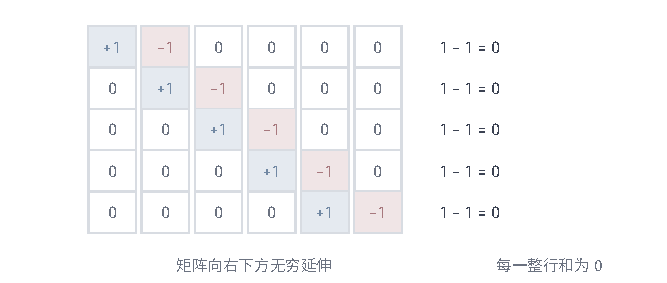
\includegraphics[width=112mm]{figures/00-shared/mathematical-preliminaries-upper/00-shared/tikz/mathematical-language-combinatorics-analysis-optimization-comprehension-additions/fubini-cancellation-grid.pdf}
  \caption{无穷矩阵$a_{i,j}=\mathbb I\{j=i\}-\mathbb I\{j=i+1\}$的左上角，展示前五行、前六列，矩阵向右下方继续；每个单元格也可看成第一象限中边长为$1$的方格。每一整行的和为$0$；第一整列的和为$1$，其他整列的和为$0$。蓝、红单元分别为$+1,-1$，每行绝对和为$2$，因而无穷矩阵不绝对可加。}
  \label{fig:vol1-add-fubini-cancellation-grid}
\end{figure}

连续函数也会出现同样的现象。
\begin{example}[$(x^2-y^2)/(x^2+y^2)^2$的两种累次积分不同]
\label{ex:region-rational-non-fubini}
在$(0,1)^2$上取
\[
 f(x,y)=\frac{x^2-y^2}{(x^2+y^2)^2}.
\]
直接求导可得$\partial_y\bigl(y/(x^2+y^2)\bigr)=f(x,y)$，所以固定$x>0$时
\[
 \int_0^1f(x,y)\,\mathrm dy=\left[\frac{y}{x^2+y^2}\right]_{y=0}^{y=1}=\frac{1}{1+x^2},
\]
再对$x$积分得到$\pi/4$。
由于$f(y,x)=-f(x,y)$，先对$x$积分时内层结果是$-1/(1+y^2)$，这一次序得到$-\pi/4$。

两个结果不同，原因仍是绝对可积性失效。
在$0<y<x$处$f>0$，所以
\[
 \int_0^1|f(x,y)|\,\mathrm dy\geq\int_0^xf(x,y)\,\mathrm dy=\left[\frac{y}{x^2+y^2}\right]_{y=0}^{y=x}=\frac{1}{2x},
\]
而$\int_0^11/(2x)\,\mathrm dx=+\infty$，由Tonelli定理，$\int_{(0,1)^2}|f|\,\mathrm dm_2=+\infty$。
\end{example}

在极坐标下$|f|=|\cos2\theta|/r^2$，这正是示例~\ref{ex:region-power-function-threshold}中$p=2$的临界幂次：原点附近正负两部分各自累计无穷。

\subsection{区域积分的换元}
\label{sec:multivariable-change-variables}

累次积分保留原坐标，只改变累计次序。
换元则用一个向量值映射$T$改变位置的坐标表示，例如用半径与角度描述圆盘中的点。
换坐标以后，函数要按新坐标重写，每个小块的体积也要重新计算：参数空间中大小相同的小块，映到原空间后可能大小不同。

\subsubsection{换元公式与适用条件}

\paragraph{体积的局部缩放}

一元换元$x=T(t)$中，参数的小区间$[t,t+\Delta t]$被映成长约$|T'(t)|\Delta t$的小区间，因子$|T'(t)|$记录长度的缩放。
多元换元要把参数空间中的小块换成体积，先看线性映射。
方阵$\bm A$把单位正方体映成由$\bm A$的各列张成的平行多面体，其体积为$|\det\bm A|$；更一般地，对任意可测集合$E$都有$m_d(\bm AE)=|\det\bm A|\,m_d(E)$\scite{math-folland1999real}。

几个特例可以直接核对。
对角矩阵$\operatorname{diag}(a_1,\ldots,a_d)$分别伸缩各坐标，体积比例为$\prod_j|a_j|$，这正是坐标盒的体积规则。
正交矩阵（旋转与反射）保持距离，不改变图形的形状和大小，行列式为$\pm1$。
剪切矩阵$\begin{bmatrix}1&s\\0&1\end{bmatrix}$把正方形推成等底等高的平行四边形，面积不变，行列式也等于$1$。
公式取行列式的绝对值，是因为反射这类改变定向的映射行列式为负，而体积必须非负。

对可微的非线性映射$T$，在一点$\bm x$附近有$T(\bm x+\bm h)=T(\bm x)+\bm J_T(\bm x)\bm h+o(\lVert\bm h\rVert_2)$，其中$\bm J_T$是Jacobian矩阵。局部线性近似可参考\BookChapterRef{chap:multivariate-calculus}{卷一“多元函数微分”章}。
于是以$\bm x$为角、边长为$\varepsilon$的小方块$Q$，被$T$映成一个近似的平行多面体，其体积约为$|\det\bm J_T(\bm x)|\varepsilon^d$。

设$g$是原空间中的密度。用小方块$Q_k$铺满参数区域，记$\bm x_k$为$Q_k$的一个角，每块映成的小块$T(Q_k)$中的质量约为
\[
 g(T(\bm x_k))\,m_d(T(Q_k))\approx g(T(\bm x_k))|\det\bm J_T(\bm x_k)|\varepsilon^d.
\]
对$k$求和后，左侧的和近似原空间中的总质量，右侧的和近似参数空间中函数$g(T(\bm x))|\det\bm J_T(\bm x)|$的积分。
因此$g\circ T\,|\det\bm J_T|$是“每单位参数体积所含的质量”：它把原空间中按单位体积计的密度，换算成按参数小块计的密度。

这个局部说明还不是整个积分公式的证明。
整体上还必须控制每块的近似误差在加总以后趋于零，并且确保$T$把每个点只覆盖一次：若两个参数小块映到同一块正体积区域，那里的质量就会被计算两次。

\paragraph{勒贝格积分的换元}

开集之间的$C^1$微分同胚同时满足这两项要求：连续可微保证局部的体积规则，双射保证全局只覆盖一次。
定理直接对勒贝格可测函数陈述，连续被积函数是其特例。
\begin{theorem}[区域积分的换元公式]
设$U,V\subseteq\mathbb R^d$为开集，$T:U\to V$为$C^1$双射，逆映射也为$C^1$，且$\det\bm J_T$处处非零。
对任意非负勒贝格可测函数$g:V\to[0,\infty]$，有
\begin{equation}
 \int_Vg(\bm y)\,\mathrm d\bm y
 =\int_Ug(T(\bm x))|\det\bm J_T(\bm x)|\,\mathrm d\bm x,
 \label{eq:measurable-change-variables}
\end{equation}
允许共同值为$+\infty$。若$g$有符号且在$V$上绝对可积，则变换后的函数也绝对可积，等式仍成立并取有限值。
\end{theorem}

这类变换及其逆在定义域的每个闭有界子集上满足Lipschitz条件，因而把零测集映为零测集。
所以勒贝格可测函数$g$与$T$复合后仍勒贝格可测：Borel集合的原像仍是Borel集合，零测集的原像仍是零测集，而每个勒贝格可测集都是Borel集合与零测集子集之并。

一般定理先建立可测集合的体积变换$m_d(T(E))=\int_E|\det\bm J_T|$，再从指示函数进入简单函数，最后以单调逼近得到非负函数的公式；有符号情形对$|g|$、$g^+$和$g^-$分别应用非负结论即可。
这里说明的是证明的依赖关系，集合层的体积变换定理引用测度论教材\scite{math-folland1999real}，不把逐点线性化当作完整证明。

若只在可测子区域$D\subseteq U$上积分，对$V$中的函数$g\mathbb I_{T(D)}$应用同一公式，即得
\begin{equation}
 \int_{T(D)}g(\bm y)\,\mathrm d\bm y
 =\int_Dg(T(\bm x))|\det\bm J_T(\bm x)|\,\mathrm d\bm x.
 \label{eq:analysis-multivariate-change-variables}
\end{equation}
这里不另加有界或边界零测的要求；所需条件仍是非负可测，或者有符号且绝对可积。

常用坐标在原点、坐标轴或角度的接缝处不是微分同胚，例如极坐标在原点处所有角度都对应同一点。
若在参数区域和原区域中各去掉一个零测集以后，参数化成为开集之间的$C^1$微分同胚，就可以先在剩下的范围内换元，再补回零测集，因为零测集对积分没有贡献。
若参数化在正测度区域上重复覆盖，则不能直接使用这个单次覆盖版本。

\subsubsection{常用坐标变换}

\paragraph{极坐标}

圆盘的边界用直角坐标描述时，积分上下限会含平方根。
以半径$r$和角度$\theta$作为坐标，圆盘变成参数矩形$[0,1]\times[0,2\pi]$，但面积权重必须增加半径因子。
在平面上画出同心圆$r=$常数与射线$\theta=$常数组成的网格：介于$r$与$r+\Delta r$、$\theta$与$\theta+\Delta\theta$之间的小块，径向边长为$\Delta r$，弧向边长约为$r\Delta\theta$，所以面积约为$r\Delta r\Delta\theta$。
同样大小的参数块，离原点越远，对应的面积越大；靠近原点时则被压缩得很小。
这一面积权重正是极坐标映射的Jacobian行列式：直接求导得到$\det\bm J=r$。下面用它计算单位圆盘的面积，并检查换元公式的条件。
\begin{example}[用极坐标计算单位圆盘的面积]
\label{ex:analysis-polar-coordinate-jacobian}
令$D=\{\bm x\in\mathbb R^2:\lVert\bm x\rVert_2\leq1\}$，并令$T(r,\theta)=(r\cos\theta,r\sin\theta)$。
在开集$U=(0,1)\times(0,2\pi)$上，$T$是到$V$的$C^1$双射，逆映射也是$C^1$，其中$V$是开圆盘去掉线段$[0,1)\times\{0\}$（含原点）后的区域。
直接计算可得$|\det\bm J_T(r,\theta)|=r$，在$U$上处处非零。
$D$与$V$只相差边界圆周和线段$[0,1)\times\{0\}$，它们都是零测集，因此
\[
 \int_D1\,\mathrm d\bm x
 =\int_V1\,\mathrm d\bm x
 =\int_0^{2\pi}\int_0^1r\,\mathrm dr\,\mathrm d\theta
 =\pi.
\]
最后一步在参数矩形上使用Tonelli定理，积分上下限包含端点不改变积分值。
若让$\theta$取遍$(0,4\pi)$，圆盘就会被覆盖两次，按公式算出的$2\pi$不再是面积，这正是单次覆盖条件排除的情形。
\end{example}

图~\ref{fig:vol1-add-polar-area-weight}说明半径因子来自哪里。同样的角度变化在较大半径处扫过更长的弧，故同样大小的参数块对应更大的面积，积分权重必须随半径变化。
\begin{figure}[!htb]
  \centering
  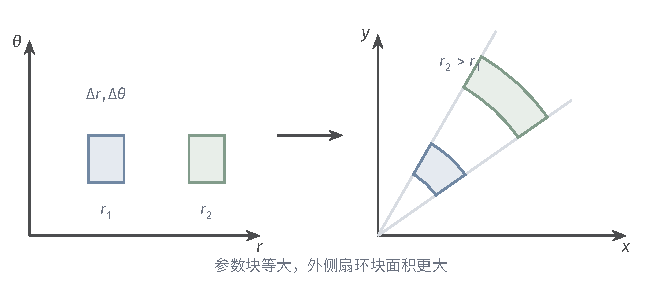
\includegraphics[width=112mm]{figures/00-shared/mathematical-preliminaries-upper/00-shared/tikz/mathematical-language-combinatorics-analysis-optimization-comprehension-additions/polar-area-weight.pdf}
  \caption{极坐标映射中的两个等大参数块，具有相同的$\Delta r,\Delta\theta$，但外侧半径$r_2$较大。对应扇环块的精确面积为$(r\Delta r+(\Delta r)^2/2)\Delta\theta$，一阶项为$r\Delta r\Delta\theta$，因此面积元为$r\,\mathrm dr\,\mathrm d\theta$。图只比较局部块，坐标原点与接缝的处理见正文。}
  \label{fig:vol1-add-polar-area-weight}
\end{figure}

用极坐标可以直接核对示例~\ref{ex:region-power-function-threshold}得到的阈值。
\begin{example}[用极坐标核对幂函数的可积阈值]
\label{ex:region-polar-power-check}
设$0<a<b$，在圆环$\{a\leq\lVert\bm x\rVert_2\leq b\}$上积分$\lVert\bm x\rVert_2^{-p}$。
在开集$(a,b)\times(0,2\pi)$上使用极坐标，被去掉的两条圆周和一条线段都是零测集；被积函数只依赖半径，于是
\[
 \int_{a\leq\lVert\bm x\rVert_2\leq b}\lVert\bm x\rVert_2^{-p}\,\mathrm d\bm x
 =\int_0^{2\pi}\int_a^br^{-p}\cdot r\,\mathrm dr\,\mathrm d\theta
 =2\pi\int_a^br^{1-p}\,\mathrm dr.
\]
令$a\downarrow0$，它有界当且仅当$1-p>-1$，即$p<2$；令$b\to\infty$，它有界当且仅当$1-p<-1$，即$p>2$，与壳层估计一致。
取$p=0$、$a=1$、$b=2$，得到$2\pi\int_1^2r\,\mathrm dr=3\pi$，这就是示例~\ref{ex:region-power-function-threshold}中的$\alpha=m_2(A_0)$。
\end{example}

面积因子$r$正是壳层估计中“面积随半径增长”的来源：半径约为$r$、厚度为$\Delta r$的细圆环，面积约为$2\pi r\Delta r$。

极坐标与累次积分结合，还能计算一个没有初等原函数的一元积分。
\begin{example}[用极坐标计算Gauss积分]
\label{ex:region-gauss-integral}
函数$e^{-x^2}$没有初等原函数，但平面函数$e^{-(x^2+y^2)}$非负，在极坐标下只依赖半径。
对开集$(0,\infty)\times(0,2\pi)$使用换元公式，被去掉的原点和正$x$轴是零测集，于是
\[
 \int_{\mathbb R^2}e^{-(x^2+y^2)}\,\mathrm d(x,y)
 =\int_0^{2\pi}\int_0^\infty e^{-r^2}r\,\mathrm dr\,\mathrm d\theta
 =2\pi\cdot\frac12=\pi.
\]
另一方面，由Tonelli定理，左侧等于
\[
 \begin{aligned}
 \int_{\mathbb R}\left(\int_{\mathbb R}e^{-x^2}e^{-y^2}\,\mathrm dy\right)\mathrm dx
 &=\int_{\mathbb R}e^{-x^2}\,\mathrm dx\cdot\int_{\mathbb R}e^{-y^2}\,\mathrm dy\\
 &=\left(\int_{\mathbb R}e^{-x^2}\,\mathrm dx\right)^2.
 \end{aligned}
\]
这个积分为正，因此$\int_{\mathbb R}e^{-x^2}\,\mathrm dx=\sqrt\pi$。
\end{example}

这个结果给出正态分布密度的归一化常数。
计算同时用到了换元和累次积分：换元把平面积分变成可算的径向积分，累次积分把同一个平面积分拆成两个相同的一元积分。

\paragraph{柱坐标}

在三维中，柱坐标在极坐标之外保留高度$z$：
\[
 (x,y,z)=(r\cos\theta,r\sin\theta,z).
\]
参数小块对应的是一块极坐标小块再沿竖直方向拉高$\Delta z$，体积约为$r\Delta r\Delta\theta\Delta z$。
Jacobian矩阵左上角是极坐标的$2\times2$块，右下角为$1$，其余元素为零，行列式仍为$r$，故体积元是$r\,\mathrm dr\,\mathrm d\theta\,\mathrm dz$。
用这个体积元可以直接算出圆柱体的体积。
\begin{example}[圆柱体的体积]
\label{ex:region-cylinder-volume}
半径$R$、高度$H$的圆柱体由$0\leq r\leq R$、$0\leq\theta\leq2\pi$、$0\leq z\leq H$描述。
与极坐标相同，在开参数长方体$(0,R)\times(0,2\pi)\times(0,H)$上换元，去掉的竖直半平面片和圆柱表面都是零测集。于是
\[
 \int_0^H\int_0^{2\pi}\int_0^R r\,\mathrm dr\,\mathrm d\theta\,\mathrm dz
 =H\cdot2\pi\cdot\frac{R^2}{2}=\pi R^2H.
\]
\end{example}

关于竖直轴对称的物体，如圆柱、圆锥、旋转抛物面所围的区域，用柱坐标描述时上下限最简单。

\paragraph{球坐标}

球坐标用到原点的距离$\rho$、从正$z$轴量起的夹角$\varphi$和绕$z$轴的角$\theta$：
\[
 (x,y,z)=(\rho\sin\varphi\cos\theta,\rho\sin\varphi\sin\theta,\rho\cos\varphi).
\]
在球面上，$\varphi$相当于纬度（从北极量起），$\theta$相当于经度。
参数小块对应的近似长方体有三条边：沿径向长$\Delta\rho$；沿经线长$\rho\Delta\varphi$；沿纬线圆长$\rho\sin\varphi\Delta\theta$，因为纬线圆的半径是$\rho\sin\varphi$。
三边相乘得到体积约为$\rho^2\sin\varphi\,\Delta\rho\Delta\varphi\Delta\theta$；靠近两极时纬线圆变小，参数小块对应的体积也随之变小。

按$(\rho,\varphi,\theta)$的次序写出Jacobian矩阵，沿第三行展开行列式，
\[
 \det\begin{bmatrix}
 \sin\varphi\cos\theta&\rho\cos\varphi\cos\theta&-\rho\sin\varphi\sin\theta\\
 \sin\varphi\sin\theta&\rho\cos\varphi\sin\theta&\rho\sin\varphi\cos\theta\\
 \cos\varphi&-\rho\sin\varphi&0
 \end{bmatrix}
\]
等于
\[
 \cos\varphi\cdot\rho^2\sin\varphi\cos\varphi+\rho\sin\varphi\cdot\rho\sin^2\varphi
 =\rho^2\sin\varphi,
\]
与几何估计一致；在$0<\varphi<\pi$上它为正，故体积元为$\rho^2\sin\varphi\,\mathrm d\rho\,\mathrm d\varphi\,\mathrm d\theta$。
用这个体积元可以算出球的体积。
\begin{example}[球的体积]
\label{ex:region-ball-volume}
半径$R$的球由$0\leq\rho\leq R$、$0\leq\varphi\leq\pi$、$0\leq\theta\leq2\pi$描述。
和极坐标一样，在开参数长方体$(0,R)\times(0,\pi)\times(0,2\pi)$上换元，它覆盖的是球内部去掉半平面片$\{y=0,\ x\geq0\}$后的区域；被去掉的半平面片（其中包含$z$轴上的一段）与球面都是零测集，补回后不改变积分。于是
\[
 \int_0^{2\pi}\int_0^\pi\int_0^R\rho^2\sin\varphi\,\mathrm d\rho\,\mathrm d\varphi\,\mathrm d\theta
 =2\pi\cdot2\cdot\frac{R^3}{3}
 =\frac{4\pi R^3}{3},
\]
其中$\int_0^\pi\sin\varphi\,\mathrm d\varphi=2$，$\int_0^R\rho^2\,\mathrm d\rho=R^3/3$。
\end{example}

球在球坐标下变成参数长方体，三组上下限都是常数；以原点为中心对称的区域，或只依赖$\rho$的被积函数，用球坐标计算最简单。

\subsection{参数积分}
\label{sec:multivariable-parameter-integrals}

换元改变的是空间坐标。
参数积分则固定积分区域，让被积函数依赖一个实参数$\theta$，研究积分所得的总量怎样随参数变化。
例如$\theta$是时间，$g(\bm x,\theta)$是时刻$\theta$的质量密度，积分就是该时刻的总质量；或者$\theta$是模型中的参数，积分是依赖该参数的平均损失。
这里要回答三个问题：总量是否随参数连续变化，总量的变化率能否由密度的变化率累计得到，以及积分区间的端点也随参数移动时怎样求导。

\subsubsection{参数积分的定义}

设$D\in\mathcal L(\mathbb R^d)$，$I$为实参数区间，且对每个$\theta\in I$，$g(\cdot,\theta)$都是$D$上可积的标量函数。定义
\[
 G(\theta)=\int_Dg(\bm x,\theta)\,\mathrm d\bm x.
\]
固定参数后，$\bm x$是被积变量；积分完成以后，$G$是参数$\theta$的一元函数。
例如$D=[0,\infty)$、$g(x,\theta)=e^{-\theta x}$（$\theta>0$）时，$G(\theta)=1/\theta$。

点态连续或点态可微只描述每个固定位置$\bm x$处的变化。
总量$G$还可能因为“质量”在参数变化时移向无穷远，或集中到越来越小的区域而突变，这些现象在任何固定位置都看不出来。
下面的例子中，密度在每一点都趋于零，总质量却保持不变。
\begin{example}[$\theta e^{-\theta x}$的质量逃向无穷远]
\label{ex:region-escaping-mass}
在$[0,\infty)$上令$g(x,\theta)=\theta e^{-\theta x}$（$\theta>0$）。对每个$\theta>0$，
\[
 G(\theta)=\int_0^\infty\theta e^{-\theta x}\,\mathrm dx=1.
\]
另一方面，$\theta\downarrow0$时，对每个固定的$x$都有$g(x,\theta)\to0$。
质量被摊薄并推向远处：由$\int_c^\infty\theta e^{-\theta x}\,\mathrm dx=e^{-\theta c}$，总质量的一半位于$x\geq(\log2)/\theta$的位置，而这个位置随$\theta\downarrow0$趋于无穷远。
若在$\theta=0$处按点态极限令$g(x,0)=0$，则$G(0)=0\neq1=\lim_{\theta\downarrow0}G(\theta)$。
\end{example}

可见点态极限本身不能决定总量的极限；要把点态性质传递给$G$，还需要控制整族函数，防止质量逃逸。

\subsubsection{参数积分的连续性}

所需的控制由支配收敛定理提供：用同一个可积函数控制附近全部参数的密度，贡献就不能集中到越来越小的区域，也不能移向无穷远。
\begin{theorem}[可积控制下参数积分的连续性]
设$\theta_0\in I$，每个$g(\cdot,\theta)$可测。假设存在$\theta_0$在$I$中的一个相对邻域$J$、同一个可测零测集$N$及非负可积函数$h$，使对每个$\bm x\in D\setminus N$，$g(\bm x,\cdot)$在$\theta_0$连续，且
$|g(\bm x,\theta)|\leq h(\bm x)$对所有$\theta\in J$成立。
则$G(\theta)$在$J$上有有限值，并在$\theta_0$连续。
\end{theorem}
\begin{proof}
任取$\theta_n\to\theta_0$，充分大时$\theta_n\in J$。在$D\setminus N$上，$g(\bm x,\theta_n)\to g(\bm x,\theta_0)$，且绝对值都不超过$h(\bm x)$。
支配收敛给出$G(\theta_n)\to G(\theta_0)$，由序列判据得到连续性。
\end{proof}

控制函数$h$的作用是给所有邻近参数的密度一个共同的、总量有限的上方包络，质量就无法逃到包络以外。
示例~\ref{ex:region-escaping-mass}中不存在这样的包络：对任意$\delta>0$，当$x>1/\delta$时，
\[
 \sup_{0<\theta<\delta}\theta e^{-\theta x}=\frac{1}{ex},
\]
上确界在$\theta=1/x$处取到，而$1/(ex)$在$(1/\delta,\infty)$上不可积。

相反，对$g(x,\theta)=e^{-\theta x}$，固定$\theta_0>0$，在邻域$\theta>\theta_0/2$内有$e^{-\theta x}\leq e^{-\theta_0x/2}$，后者在$[0,\infty)$上可积，故$G$在$\theta_0$连续。
控制函数只需覆盖所考察参数点的邻域，不要求同一上界适用于全部参数；这里每个$\theta_0>0$各用一个包络，就得到$G$在整个$(0,\infty)$上连续。

\subsubsection{积分号下求导}

若$g(\bm x,\theta)$是时刻$\theta$的密度，自然希望总质量的变化率等于各处密度变化率的累计，即$G'(\theta)=\int_D\partial_\theta g(\bm x,\theta)\,\mathrm d\bm x$。
这实际是交换参数差商的极限与积分。
各点偏导数存在只确定差商的点态极限；用同一个可积函数控制全部差商，才足以将这个极限移入积分号。
\begin{theorem}[可积导数界下的积分号内求导]
设$I$是包含$\theta_0$的开区间，对每个$\theta\in I$，$\bm x\mapsto g(\bm x,\theta)$可测，并且$g(\cdot,\theta_0)$可积。
假设存在一个可测零测集$N$，使每个$\bm x\in D\setminus N$处的$\theta\mapsto g(\bm x,\theta)$在整个$I$内可微；对每个$\theta$，偏导数作为$\bm x$的函数可测，并且存在非负可积函数$h$使
\begin{equation}
 \left|\frac{\partial g}{\partial\theta}(\bm x,\theta)\right|\leq h(\bm x)
 \quad\text{对所有$\bm x\in D\setminus N$及所有$\theta\in I$成立},
 \label{eq:analysis-parameter-derivative-domination}
\end{equation}
则对每个$\theta\in I$，$g(\cdot,\theta)$在$D$上可积，且
\begin{equation}
 G'(\theta_0)=\int_D\frac{\partial g}{\partial\theta}(\bm x,\theta_0)\,\mathrm d\bm x.
 \label{eq:analysis-differentiate-under-integral}
\end{equation}
\end{theorem}
\begin{proof}
对$\bm x\notin N$，一元中值定理给出
$|g(\bm x,\theta)-g(\bm x,\theta_0)|\leq|\theta-\theta_0|h(\bm x)$，
所以$I$中每个$g(\cdot,\theta)$都被可积函数$|g(\cdot,\theta_0)|+|\theta-\theta_0|h$控制，因而可积，$G$在$I$内有有限值。
对非零$t$且$\theta_0+t\in I$，令
\[
 q_t(\bm x)=\frac{g(\bm x,\theta_0+t)-g(\bm x,\theta_0)}{t}.
\]
中值定理又给出
\[
 |q_t(\bm x)|\leq h(\bm x)\qquad(\bm x\notin N),
\]
并且$t\to0$时，$q_t(\bm x)$在$D\setminus N$上趋于$\partial g/\partial\theta(\bm x,\theta_0)$。
对任意非零序列$t_n\to0$应用支配收敛，都得到同一个积分极限$\int_D\partial_\theta g(\bm x,\theta_0)\,\mathrm d\bm x$；
由实数极限的序列判据，它就是差商$\bigl(G(\theta_0+t)-G(\theta_0)\bigr)/t$在$t\to0$时的极限，即式~\eqref{eq:analysis-differentiate-under-integral}。
\end{proof}

这里的零测集$N$和控制函数$h$都不能随参数改变：参数范围不可数，不能靠取全部参数例外集的并自动获得一个零测集。
条件~\eqref{eq:analysis-parameter-derivative-domination}是一组便于核对的充分条件；更一般的版本也可以直接控制参数差商。

控制函数通常只在所考察参数点的一个邻域内取得。
\begin{example}[对$e^{-\theta x}$在积分号下求导]
\label{ex:region-differentiate-exponential}
令$g(x,\theta)=e^{-\theta x}$，$x\in[0,\infty)$、$\theta>0$，则$G(\theta)=1/\theta$。
固定$\theta_0>0$，取$I=(\theta_0/2,3\theta_0/2)$，则对$\theta\in I$，
\[
 |\partial_\theta g(x,\theta)|=xe^{-\theta x}\leq xe^{-\theta_0x/2}=:h(x).
\]
分部积分给出$\int_0^\infty h(x)\,\mathrm dx=4/\theta_0^2<\infty$；不等式对每个$x$都成立，可取$N=\varnothing$。
由积分号下求导的定理，
\[
 G'(\theta_0)=-\int_0^\infty xe^{-\theta_0x}\,\mathrm dx=-\frac{1}{\theta_0^2},
\]
与$G(\theta)=1/\theta$的直接求导一致。
\end{example}

例中的控制函数依赖于$\theta_0$：若参数范围包含任意接近零的正数，$xe^{-\theta_0x/2}$就不再控制全部导数。
交换求导与积分所需的，只是所考察参数点附近的统一控制。

若所考察参数点附近找不到可积的导数界，交换求导与积分可能失败。
下面的反例发生在参数区间的端点$\theta=0$，考察的是右导数。
\begin{example}[参数积分中的控制函数失效]
\label{ex:analysis-parameter-integral-failure}
对$\theta\geq0$与$x\in(0,1)$，定义
\[
 g(x,\theta)=
 \begin{cases}
 \dfrac{\theta x}{x^2+\theta^2}, & \theta>0,\\[5pt]
 0, & \theta=0.
 \end{cases}
\]
在$\theta=0$处，对每个固定$x>0$，差商$g(x,\theta)/\theta=x/(x^2+\theta^2)\to1/x$，所以关于$\theta$的右偏导数都等于$1/x$，但$1/x$在$(0,1)$上不可积。
直接积分（令$u=x^2+\theta^2$）得到
\[
 G(\theta)=\frac{\theta}{2}\log\left(\frac{1+\theta^2}{\theta^2}\right)\quad(\theta>0),
 \qquad G(0)=0.
\]
于是$G(\theta)/\theta=\frac12\log(1+\theta^{-2})$在$\theta\downarrow0$时发散，$G$在$0$处没有有限右导数。
积分内的逐点右导数虽然存在，却缺少统一可积控制，因此这里不能交换右求导与积分。
\end{example}

从密度的角度看，$g(\cdot,\theta)$在$x=\theta$处取峰值$1/2$；$\theta$变小时峰值向原点移动，差商$g(\cdot,\theta)/\theta$在峰值处等于$1/(2\theta)$，它的累计随之变得无界。

\subsubsection{变限积分的求导}

积分号下求导的定理固定了积分区域。
端点也变化时，即使被积函数不依赖参数，积分仍然会变化：例如$G(\theta)=\int_0^\theta1\,\mathrm dx=\theta$的导数为$1$，而被积函数对参数的偏导数为零，只累计偏导数会遗漏端点移动的贡献。

用质量来理解：区间$[a(\theta),b(\theta)]$上的总质量有两种变化来源，一是区间内部各处的密度在变，二是端点移动时把新的位置划入或划出区间。
右端点在参数增加$\Delta\theta$时向右移动约$b'(\theta)\Delta\theta$，新划入的一小段上密度约为$g(b(\theta),\theta)$，带来质量约$g(b(\theta),\theta)b'(\theta)\Delta\theta$；左端点向右移动则划出一小段，减少质量约$g(a(\theta),\theta)a'(\theta)\Delta\theta$。
要用端点处的函数值估计这一小段的质量，被积函数需要在端点附近连续。
\begin{theorem}[变限参数积分的求导]
设$a(\theta),b(\theta)$在$\theta_0$附近可微，且$a(\theta)<b(\theta)$。
若$g(x,\theta)$和$\partial_\theta g(x,\theta)$在包含这些邻近积分区间的一个紧矩形上连续，则
\begin{equation}
 \begin{aligned}
 \frac{\mathrm d}{\mathrm d\theta}\int_{a(\theta)}^{b(\theta)}g(x,\theta)\,\mathrm dx
 &=\int_{a(\theta)}^{b(\theta)}\partial_\theta g(x,\theta)\,\mathrm dx\\
 &\quad+g(b(\theta),\theta)b'(\theta)
 -g(a(\theta),\theta)a'(\theta).
 \end{aligned}
\label{eq:measurable-moving-boundary-integral}
\end{equation}
\end{theorem}
\begin{proof}
记$a_0=a(\theta_0)$、$b_0=b(\theta_0)$。积分差可分解为
\[
 \begin{aligned}
 G(\theta)-G(\theta_0)
 &=\int_{a_0}^{b_0}\bigl[g(x,\theta)-g(x,\theta_0)\bigr]\,\mathrm dx\\
 &\quad+\int_{b_0}^{b(\theta)}g(x,\theta)\,\mathrm dx
 -\int_{a_0}^{a(\theta)}g(x,\theta)\,\mathrm dx.
 \end{aligned}
\]
短区间积分按端点次序采用有向约定。
第一项是固定区间上的参数积分：$\partial_\theta g$在紧矩形上连续，因而有界，常数界在有界区间$[a_0,b_0]$上可积，满足条件~\eqref{eq:analysis-parameter-derivative-domination}，所以第一项除以$\theta-\theta_0$后趋于$\int_{a_0}^{b_0}\partial_\theta g(x,\theta_0)\,\mathrm dx$。
$g$在紧矩形上一致连续，当$\theta\to\theta_0$时，短区间$[b_0,b(\theta)]$上的$g(x,\theta)$一致地接近$g(b_0,\theta_0)$，所以第二项等于
$g(b_0,\theta_0)[b(\theta)-b_0]+o(|b(\theta)-b_0|)$。端点的可微性保证$|b(\theta)-b_0|=O(|\theta-\theta_0|)$，所以它的差商趋于$g(b_0,\theta_0)b'(\theta_0)$。
第三项同理，并保留前面的负号，得到下端点贡献。三项相加即得公式。
\end{proof}

紧矩形上的连续性是一组便于核对的充分条件。
对一般可测函数，公式中的端点值$g(b(\theta),\theta)$需要另外赋予意义：几乎处处相等的两个函数可以在端点上取不同的值，不能从几乎处处的等价类中直接读出边界上的值。

\FloatBarrier

\section{同一空间上的测度比较}
\label{sec:measure-same-space-comparison}

假设我们已经在同一个可测空间$(X,\mathcal A)$上有了两种非负测度，比如同一个数据集上的两种分布、或同一组事件上的两种赋权。
怎样判断它们是不是“一回事”？如果不是，又差在哪里？
本节按从粗到细的顺序回答三层问题。
第一层只看零集：一种测度认为可以忽略的集合，另一种是否也能忽略。
第二层看表示：能否找到一个密度函数，用一种测度把另一种完整地写出来；写不出的部分又集中在哪里。
第三层看距离：用一个数概括两者整体差异时，不同指标各自在衡量什么。

要特别提醒：同一个可测空间只保证两种测度能对\emph{同一个事件}读数，它既不自动给出密度，也不提供任何几何距离。
零集关系和Radon–Nikodym密度、\term{Lebesgue分解}对一般非负$\sigma$有限测度就有意义；为了描述“两测度之差”，我们会引入允许取负值的有符号测度；再往后的全变差、Hellinger、KL和Wasserstein则统一以概率测度为对象。

\subsection{\term{绝对连续}、等价与\term{相互奇异}}

零集是比较两种测度时最基本的相容性信息。
本小节区分三种关系：一种测度的零集是否都是另一种的零集（单向）、两者是否恰好共享零集（双向）、以及两者的质量能否分别集中在互不相交的范围内（分离）。
它们是三种可以分别检验的关系，并不是把测度划分成几个互斥类别。

\subsubsection{绝对连续与\term{等价测度}}

\paragraph{绝对连续的定义与方向}

先问一个单向问题：只要$\mu$认为某集合没有质量，$\nu$是否也一定认为它没有质量？
若对每个可测集$A$都有
\[
 \mu(A)=0\ \Longrightarrow\ \nu(A)=0,
\]
就称$\nu$相对于$\mu$\term{绝对连续}，记作$\nu\ll\mu$。
符号的方向很重要：被比较的是“$\nu$的零集是否包含在$\mu$的零集里”。
这是对\emph{整个可测集合}提出的要求，不是比较两个密度函数逐点值的大小。

如果$\nu$已经能用一个非负可测函数相对$\mu$表示，
\[
 \nu(A)=\int_A f\,d\mu,
\]
那么在$\mu$零集上积分自然为零，立刻有$\nu\ll\mu$。
也就是说，“有密度”是绝对连续的充分条件；反过来，零集相容是否足以保证存在这样的密度函数，正是Radon–Nikodym定理要回答的。

绝对连续不是连续空间的专利，在离散集合上同样可以定义；但有两个直觉陷阱要避开。
第一个陷阱是把点质量当成绝对连续：实轴上$\delta_0$相对于勒贝格测度并不绝对连续，因为$\lambda(\{0\})=0$而$\delta_0(\{0\})=1$。
第二个陷阱是以为“检查所有单点”就够了。
取$P,Q$分别均匀分布在$[0,1]$和$[2,3]$上：每个单点在两者下质量都是零，看似零集相同，但$P([0,1])=1$而$Q([0,1])=0$，所以$P$并不对$Q$绝对连续。
原因是$[0,1]$这样的集合不可数，不能用可数可加性把它的质量拆成单点质量之和；只验证单点，覆盖不了定义中“每个可测集”的要求。

\paragraph{等价测度与共同零集}

若两个方向的绝对连续同时成立，$\mu\ll\nu$且$\nu\ll\mu$，就记作$\mu\sim\nu$，称两测度等价。
等价的含义非常具体：两者有完全相同的可测零集。
但等价\emph{不意味着相等}：同一个非零集合在两种测度下可以有很不一样的质量，只是“谁为零”完全一致。

一个常用的充分判据是：若$\nu=f\mu$且密度$f>0$在$\mu$几乎处处成立，则两测度等价。
我们已经知道$\nu\ll\mu$；反方向只需证明$\nu(A)=0\Rightarrow\mu(A)=0$。
把$\{f>0\}$按高度切成可数层$\{f\geq1/m\}$：若$\int_Af\,d\mu=0$，则
\[
 \mu\bigl(A\cap\{f\geq1/m\}\bigr)
 \leq m\int_Af\,d\mu=0
\]
对每个$m$成立；可数并起来，$A$在$\{f>0\}$内的部分质量为零，而$f>0$几乎处处成立，所以$\mu(A)=0$。
直觉上，用一个处处为正的密度重新加权，只会改变各区域的质量比例，不会把任何原本有质量的区域压成零。

\subsubsection{相互奇异}

\paragraph{相互奇异与可测集中范围}

与“共享零集”相反的另一种极端是：两种质量各占一块互不重叠的可测范围。
如果存在可测集$E$，使
\[
 \mu(X\setminus E)=0,\qquad \nu(E)=0,
\]
即$\mu$的质量几乎全在$E$上、$\nu$的质量几乎全在补集$X\setminus E$上，就称$\mu$与$\nu$\term{相互奇异}，记作$\mu\perp\nu$。

勒贝格测度与$\delta_0$就是标准例子：取$E=\mathbb R\setminus\{0\}$，连续长度全部集中在$E$上（$\{0\}$长度为零），点质量全部集中在补集$\{0\}$上。
要注意相互奇异只要求可测意义下的集中范围分离，并不要求这两个范围在几何上隔开——$E=\mathbb R\setminus\{0\}$的闭包仍是整条实轴，与$\{0\}$在拓扑上并不分离。
此外，一个测度完全可能“两张单子都有钱”：既在连续区域里铺开一部分、又在参考看不见的集合里藏一部分，于是它整体既不绝对连续也不奇异。
下一小节的Lebesgue分解就专门处理这种混合情形。

\begin{figure*}[htbp]
\centering
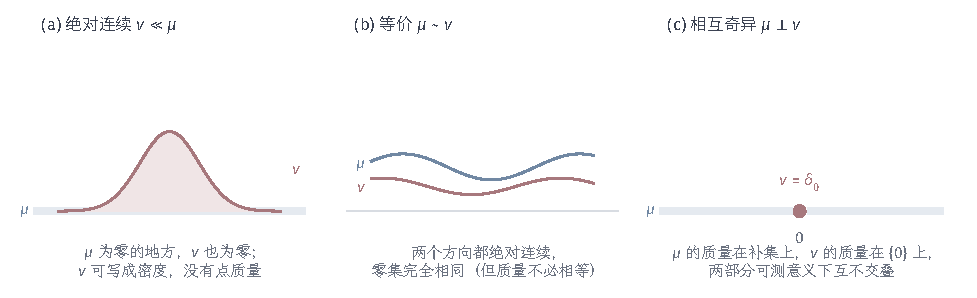
\includegraphics[width=169mm]{figures/00-shared/mathematical-preliminaries-upper/05-space-and-geometry/tikz/zero-set-relations/figure.pdf}
\caption{同一参考测度（蓝色横线）下，两种测度之间的三种零集关系。(a) 绝对连续$\nu\ll\mu$：$\nu$（红色密度）只在$\mu$有质量的地方取非零值，没有点质量。(b) 等价$\mu\sim\nu$：两个方向都绝对连续，零集完全相同，但同一区域上的质量大小仍可不同。(c) 相互奇异$\mu\perp\nu$：长度与点质量$\delta_0$各占一个可测范围，在可测意义下互不交叠。}
\label{fig:zero-set-relations}
\end{figure*}

\subsection{相对密度与测度分解}

本小节回答四个递进的问题：在什么条件下能找到密度、密度上的数值到底代表什么、怎样用它改写积分、以及当整个测度不能由密度表示时怎样把它拆开。
需要强调，这里的“导数”$d\nu/d\mu$是\emph{两种积分权重之比}，与坐标对坐标的普通导数没有关系。

\subsubsection{相对密度的存在与几乎处处唯一}

\paragraph{相对密度的存在与有限性}

绝对连续只告诉我们零集相容，我们还希望更具体：用一个函数$f$就能恢复$\nu$在\emph{每一个}可测集上的质量。

\begin{theorem}[Radon–Nikodym定理]
\label{thm:measure-radon-nikodym}
设$\mu,\nu$是同一可测空间上的非负$\sigma$有限测度，且$\nu\ll\mu$。
则存在非负可测函数$f$，使
\[
 \nu(A)=\int_A f\,d\mu\qquad(A\in\mathcal A).
\]
\end{theorem}

这个$f$记作$\dfrac{d\nu}{d\mu}$，称为$\nu$相对于$\mu$的\term{Radon–Nikodym密度}。
它的直觉是：在$x$附近取一个很小的可测块，$\nu$给这块的质量约等于$f(x)$乘以$\mu$给它的质量，密度就是两种称重方式在局部的换算比例。
$\sigma$有限是本定理常用的充分条件，不应说成一切密度存在的必要条件；对已经写出连续密度或离散权重的情形，那个已知函数本身就是Radon–Nikodym密度。

目标测度$\nu$的$\sigma$有限性还能保证密度不取无穷值。
设$E_k$覆盖$X$且$\nu(E_k)<\infty$，考虑$N=\{f=\infty\}$：
若$\mu(N\cap E_k)>0$，则$\nu(E_k)=\int_{E_k}f\,d\mu\geq+\infty$，矛盾。
故每个$N\cap E_k$都是$\mu$零集，可数并得$\mu(N)=0$。
因此总可以选一个几乎处处有限的代表，这也为后面等价测度取倒数做了准备。

\paragraph{密度的几乎处处唯一}

密度只在“零测集可以忽略”的意义下唯一。
若$f,g$都恢复$\nu$，把空间切成有限质量块、再把函数取值切成有界层和严格间隔层，就能在每一块上比较。
关键一步是：在某个$f\geq g+1/m$的可测层$D$上，两种表示给出
\[
 \int_Df\,d\mu=\nu(D)=\int_Dg\,d\mu,
\]
但若$\mu(D)>0$，左侧至少比右侧多$\mu(D)/m>0$，矛盾，所以$D$是零集。
可数合并所有块、所有层，得到$f>g$和$g>f$的集合都是零集，即
\[
 \frac{d\nu}{d\mu}=f=g\qquad\mu\text{几乎处处}.
\]
在$\mu$零集上随意改动密度值不影响任何集合的测度，所以密度并不规定每一个点上的数值，只规定“几乎处处”的局部比例。

\subsubsection{密度值与单点质量}

\paragraph{密度系数与单点质量的区别}

密度描述的是质量\emph{怎样沿集合分布}，不是“某一点上的概率”，这两者很容易混淆。
若$\nu=f\mu$且$\{x\}$可测，则
\[
 \nu(\{x\})=\int_{\{x\}}f\,d\mu.
\]
等式两边是不同对象：右边是用密度系数在单点上累计出的质量。

在$[0,1]$上取概率密度$p(x)=1$和$q(x)=2x$。
两者给每个单点的质量都是零，但在区间$[0,1/2]$上的质量不同：
\[
 \int_0^{1/2}1\,dx=\frac12,\qquad
 \int_0^{1/2}2x\,dx=\frac14.
\]
可见密度值大并不代表该点概率大，密度控制的是一整段区域的质量。

只有当参考测度在单点上本身有正质量，即$0<\mu(\{x\})<\infty$时，单点上的积分才退化为乘法$f(x)\mu(\{x\})$，此时
\[
 f(x)=\frac{\nu(\{x\})}{\mu(\{x\})}
\]
才真正是两点质量之比——离散权重表中的相对频率正是这种情形。
反过来，若$\mu(\{x\})=0$，随便改$f(x)$都不会改变测度。

用$\delta_0$还能看清密度表示的边界：任何普通非负函数$f$在单点$\{0\}$上的勒贝格积分都是$0$，不可能恢复$\delta_0(\{0\})=1$，所以$\delta_0$没有相对勒贝格测度的普通密度。
广义函数里的Dirac-$\delta$要在分布理论中另立框架，不能当成Radon–Nikodym可测函数；同理，也不能指望“在某个点填一个无穷大密度值”就表示出点质量。

\subsubsection{积分的换测度公式}

\paragraph{用相对密度改写积分}

有了密度$f=d\nu/d\mu$，对$g$的积分就能换一种参考测度来算：
\[
 \int_X g\,d\nu=\int_X gf\,d\mu.
\]
这个等式先对指示函数$g=\mathbf 1_A$成立（它就是Radon–Nikodym表示本身），再对简单函数由线性成立，最后对一般非负可测$g$由单调逼近成立，允许两边同为$+\infty$。
它做的事情只是“换一杆秤来称同一个函数”，输入点没有移动，输出集合也没有重新生成。
对有符号$g$则分别处理正负部分，在不会出现$+\infty-(+\infty)$时合并；特别地
\[
 \int|g|\,d\nu=\int|g|f\,d\mu
\]
把两种写法下的绝对可积条件对齐。

\paragraph{重加权、限制与归一化}

换测度公式反过来用就是“造一个新测度”：取非负可测权重$w$，定义
\[
 \nu(A)=\int_Aw\,d\mu.
\]
可数可加性由指标上的可加性和单调收敛保证。
若总权重$Z=\int_Xw\,d\mu$满足$0<Z<\infty$，归一化后$Q(A)=\nu(A)/Z$就是概率测度，密度为$w/Z$；$Z=0$或$Z=+\infty$时无法这样归一化。

取$w=\mathbf 1_E$得到\term{限制测度}$\mu_E(A)=\mu(A\cap E)$，归一化后就是“只在$E$内部按原相对比例分配质量”的条件分布。
注意三种“限制”的区别：乘以权重改变的是赋权、底集不变；推前测度会把输入点送到另一个空间；限制到子$\sigma$代数则只是减少可见集合。
在$[0,1]$均匀概率下取$w=2\mathbf 1_{[0,1/2]}$，得到的概率把全部质量放在前半段，它对原测度绝对连续，却不再等价——原来有质量的后半段被压成了零。

\paragraph{链式换参考与倒数公式}

密度可以像换算单位一样连乘。
若$\rho\ll\nu\ll\mu$，对集合指标连续换两次参考，得到链式法则
\[
 \frac{d\rho}{d\mu}=\frac{d\rho}{d\nu}\frac{d\nu}{d\mu}
 \qquad\mu\text{几乎处处},
\]
在密度为零处把乘积约定为零，避免无意义的$0\cdot\infty$。

如果两测度等价$\mu\sim\nu$，密度$f=d\nu/d\mu$不仅几乎处处非零，还几乎处处有限，于是可以取倒数。
对可测集$B$，
\[
 \int_B\frac1f\,d\nu=\int_B\frac1f\,f\,d\mu=\mu(B),
\]
所以$d\mu/d\nu=1/f$在$\nu$几乎处处成立。
单向绝对连续不足以走到这一步——密度可能在一整块区域上为零，倒数会爆炸。
用常数权重检验方向最直观：$\nu=2\mu$、$\rho=3\nu$时，$d\nu/d\mu=2$、$d\rho/d\nu=3$、$d\rho/d\mu=6$，反向$d\mu/d\nu=1/2$。
这些公式的依据始终是“恢复所有可测集上的质量”，不能形式地把微分符号当分数约掉。

\subsubsection{Lebesgue分解}

\paragraph{绝对连续部分与奇异部分}

拿一杆参考秤$\mu$去称一个新测度$\nu$，最理想的情况是处处都有换算密度。
但现实中$\nu$可能是两笔性质完全不同的“钱”：一笔均匀摊开、能用面积密度按平方计费，另一笔却集中放在个别点上、只按个数收固定费用。
拿面积秤去称第二笔，读数恒为零，怎么乘密度都乘不出那笔固定费用。
最典型的例子就是
\[
 \nu=\lambda+\delta_0,
\]
它给开区间$(a,b)$（不含$0$）的读数是长度$b-a$，却给单点$\{0\}$读数$1$。
所以整体地问“$\nu$有没有密度”会得到尴尬答案：它一部分能写成密度、另一部分写不成。

Lebesgue分解的作用，就是把这两笔账干净地分开：

\begin{theorem}[Lebesgue分解]
\label{thm:measure-lebesgue-decomposition}
设$\mu,\nu$是同一可测空间上的非负$\sigma$有限测度。
则存在唯一的非负测度$\nu_{\mathrm{ac}},\nu_{\mathrm s}$，使
\[
 \nu=\nu_{\mathrm{ac}}+\nu_{\mathrm s},\qquad
 \nu_{\mathrm{ac}}\ll\mu,\qquad
 \nu_{\mathrm s}\perp\mu.
\]
\end{theorem}

绝对连续部分再用Radon–Nikodym定理写成$\nu_{\mathrm{ac}}=f\mu$，于是每个集合的质量都拆成两笔：
\[
 \nu(A)=\int_Af\,d\mu+\nu_{\mathrm s}(A).
\]
两个定理的分工要分清：Lebesgue分解负责把“能连续表示的”和“必须单独放的”分开，Radon–Nikodym只负责表示其中的第一部分。
当奇异部分非零时，$f$不能称为整个$\nu$的密度。

\begin{figure*}[htbp]
\centering
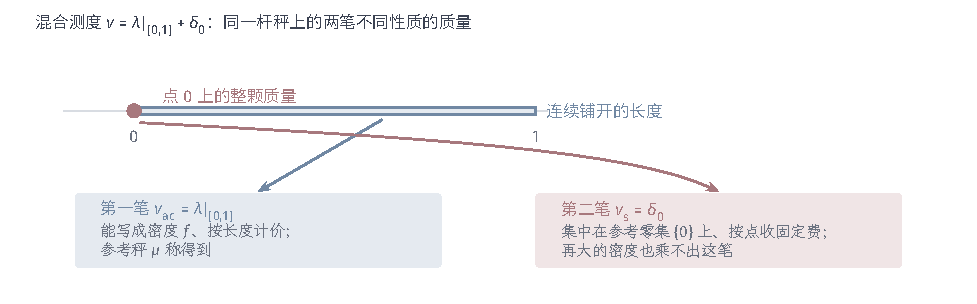
\includegraphics[width=169mm]{figures/00-shared/mathematical-preliminaries-upper/05-space-and-geometry/tikz/lebesgue-decomposition/figure.pdf}
\caption{Lebesgue分解像把混合收入拆成两笔计价规则不同的账。$\nu=\lambda|_{[0,1]}+\delta_0$中，连续铺开的长度$\nu_{\mathrm{ac}}$可以写成密度、按长度计价，参考测度$\mu$称得到；集中在参考零集$\{0\}$上的点质量$\nu_{\mathrm s}$按点收固定费，任何普通密度都乘不出这笔。每个集合收到的总质量等于两笔之和。}
\label{fig:lebesgue-decomposition}
\end{figure*}

\paragraph{分解的示例与参考测度依赖}

再看$[0,1]$上参考$\mu=\lambda|_{[0,1]}$、$\nu=\lambda|_{[0,1]}+\delta_0$这个例子，两部分的归属一目了然：铺在区间上的长度对$\mu$绝对连续（按面积的那笔），点$0$上的质量与$\mu$奇异（固定费那笔），所以
\[
 \nu_{\mathrm{ac}}=\lambda|_{[0,1]},\qquad \nu_{\mathrm s}=\delta_0.
\]
不含$0$的区间只收到长度$b-a$，集合$\{0\}$只收到点质量$1$，含$0$的区间则两笔都要算。

更通俗地说，Lebesgue分解有点像会计把一笔混合收入拆成“按面积结算”和“按点结算”两张单子：只要报上来的还是同一空间的集合，两张单子合起来就是总收入，可两张单子的计价规则谁也代替不了谁。

哪张单子非空，取决于你选用哪杆参考秤，所以分解是相对于所选参考而言的，不是测度自带的标签。
同一个$\nu$，若改取参考$\mu'=\nu$，那么每一笔质量都能按“自己称自己”换算，密度恒为$1$、奇异部分为零。
还要再次强调：奇异部分不必是孤立点；在更一般的例子里它可以由不可数个点组成、自身完全连续，却整体铺在一个参考零集上（例如后面会遇到的康托尔集）。

\subsection{有限有符号测度与全变差}

要量化两个非负测度的差异，最直接的想法是逐集合相减。
但相减的结果允许为负，不再是测度；我们需要先弄清这种“带符号的集合赋权”具有什么结构，它的正负部分和绝对变化总量怎样定义，然后才能用它给出概率之间的\term{全变差距离}。

\subsubsection{有限有符号测度与\term{总变差测度}}
\label{sec:measure-signed-total-variation}

\paragraph{集合赋权的正负分量}

对两个有限非负测度，定义
\[
 \eta(A)=\mu(A)-\nu(A).
\]
它仍然可数可加，但$\eta(A)$可以是负数。
这种取有限实值、可数可加的集合赋权称为有限\term{有符号测度}。
请注意区分：这里允许取负值的是\emph{给集合的赋权本身}，与“函数有正有负、但积分测度仍非负”是两回事。

\begin{theorem}[\term{Hahn分解}与\term{Jordan分解}]
\label{thm:measure-hahn-jordan}
对有限有符号测度$\eta$，存在互不相交且并为$X$的可测集$E_+,E_-$，使$\eta$在$E_+$的每个可测子集上非负、在$E_-$的每个可测子集上非正。
令
\[
 \eta^+(A)=\eta(A\cap E_+),\qquad
 \eta^-(A)=-\eta(A\cap E_-),
\]
则$\eta^+,\eta^-$是相互奇异的非负有限测度，且
\[
 \eta=\eta^+-\eta^-;
\]
这两个Jordan分量作为测度是唯一的。
\end{theorem}

Hahn分解选出的正负区域可以不唯一，但由此得到的正、负分量测度唯一。
可以用一张“结账表”来想这件事：同一批事件上，有的项目要额外收费（正分量）、有的项目给退款（负分量），Jordan分解就是把这张表拆成“收费单”和“退款单”两张分别只含正数的单子；总营业额是两单之差，账面上净收$0$只说明两单金额相等，绝不等于什么都没发生。
例如$\eta=\delta_0-\delta_1$在$\{0\}$上为$+1$、在$\{1\}$上为$-1$，全空间总和为$0$，可这个“总和为零”绝不意味着$\eta$处处为零。
也请把Jordan分解与Lebesgue分解区分开：前者按\emph{正负号}拆分一张有收有退的账单，后者按\emph{按面积还是按点计费}拆分一笔非负收入，两种拆分服务于不同问题。

\paragraph{总变差测度与有符号积分}

把正负部分重新加起来，得到总变差测度和\term{总变差范数}：
\[
 |\eta|=\eta^++\eta^-,\qquad
 \|\eta\|_{\mathrm{var}}=|\eta|(X).
\]
对集合$A$的任意有限分割，各块绝对赋权之和不超过$|\eta|(A)$，而按$A\cap E_+$、$A\cap E_-$分割恰好取等号；因此$|\eta|(A)$也是“把$A$切成任意小块后，绝对质量总和”的最大值。
它的作用是累计正负变化、不让它们抵消：$\eta(X)=0$时总变差仍可能很大。

对满足$\int|g|\,d|\eta|<\infty$的可测函数，定义对有符号测度的积分
\[
 \int g\,d\eta=\int g\,d\eta^+-\int g\,d\eta^-,
\]
于是
\[
 \left|\int g\,d\eta\right|\leq\int|g|\,d|\eta|
 \leq\|g\|_\infty\|\eta\|_{\mathrm{var}}.
\]
这说明要控制一个有符号赋权的积分读数，必须看它的总变差，不能只看可能正负抵消的净值$\eta(X)$。
特别地，若$\eta(A)=\int_Af\,d\mu$且$f$可积，则$f^+\mu$和$f^-\mu$正是它的Jordan分量，故$|\eta|=|f|\mu$，这把有符号测度又接回了熟悉的非负积分。

\subsubsection{全变差距离与测试积分}

现在专门比较两个概率测度$P,Q$。
先引入一个共同参考会很方便：令$\lambda=P+Q$。
因为$P,Q$都是有限测度且都对$\lambda$绝对连续，由Radon–Nikodym定理可写
\[
 p=\frac{dP}{d\lambda},\qquad q=\frac{dQ}{d\lambda}.
\]
在这个共同参考下，两者密度之差$p-q$的正负部分恰好等重——这会带来全变差特有的$1/2$系数。

\paragraph{事件质量差与密度公式}

最直接的比较，是看两个概率在同一个事件上的读数最多差多少：
\[
 \operatorname{TV}(P,Q)=\sup_{A\in\mathcal A}|P(A)-Q(A)|.
\]
它只关心“同一事件、两种权重”，不涉及事件在空间中的位置。
由概率质量介于$0,1$之间可知$0\leq\operatorname{TV}\leq1$；对称性、三角不等式和“距离为零即两测度相同”都可直接验证，所以TV是概率测度间的真正距离。

为什么它又等于密度差的$L^1$距离的一半？令$h=p-q$。
因为总质量都是$1$，$\int h\,d\lambda=0$，$h$的正部总量等于负部总量。
取正差集合$A_+=\{p\geq q\}$，任何事件上的质量差都不超过正部总量，而$A_+$恰好达到它；正负两部分合在一起得
\[
 \operatorname{TV}(P,Q)
 =\frac12\int|p-q|\,d\lambda
 =\frac12|P-Q|(X).
\]
$1/2$来自两个概率总质量相等（正差、负差各算一次才是$\int|p-q|$）；换成另一个共同有限参考，事件差上确界不变，所以数值与参考选择无关。
但若比较的是总质量不等的一般有限测度，这个$1/2$约定就要重新考虑。

\paragraph{有界观测量的误差控制}

TV之所以有用，是因为它立刻控制有界函数的期望误差。
若$g$取值在$[a,b]$内，先减去常数$(a+b)/2$再用密度差估计：
\[
 \left|\int g\,dP-\int g\,dQ\right|
 \leq(b-a)\operatorname{TV}(P,Q).
\]
特别地，$0\leq g\leq1$时系数为$1$，而正差集合的示性函数正好达到上确界，所以
\[
 \operatorname{TV}(P,Q)=\sup_{0\leq g\leq1}\left|\int g\,dP-\int g\,dQ\right|.
\]
若改用归一化$\|g\|_\infty\leq1$，系数则为$2$。
这两个“测试函数”表示后面比较测度核时还会用到。
几何上，TV只认事件不认位置：$a\neq b$时$\operatorname{TV}(\delta_a,\delta_b)=1$，无论两点离得近还是远；这个缺口正是\term{Wasserstein距离}要补的。

\subsection{\term{Hellinger距离}与KL散度}

全变差累计的是密度的绝对差$|p-q|$。
同样在共同参考下比较密度，还可以换成别的函数：对平方根差累计得到Hellinger距离，对有向对数比求期望得到KL散度。
它们衡量的是密度差异的不同侧面，因此性质也不同。

\subsubsection{Hellinger距离}

\paragraph{平方根密度与参考无关性}

定义
\[
 H^2(P,Q)=\frac12\int(\sqrt p-\sqrt q)^2\,d\lambda,
\qquad H(P,Q)=\sqrt{H^2(P,Q)}.
\]
用$\int p=\int q=1$展开，可化成更便于计算的形式
\[
 H^2(P,Q)=1-\int\sqrt{pq}\,d\lambda.
\]
其中$\int\sqrt{pq}$是密度的“几何平均重叠”，由Cauchy–Schwarz不等式介于$0,1$之间，所以$0\leq H\leq1$。
$H$只在$P,Q$共享的质量区域上统计重叠，与共同参考的选择无关。

\paragraph{距离性质与端点情形}

非负性、对称性显然；$H=0$等价于$\sqrt p=\sqrt q$几乎处处，即两概率相同。
三角不等式可在三者统一参考$P+Q+R$下，对平方根差用Cauchy–Schwarz证明。
两个端点也很直观：$P=Q$时$H=0$；$P\perp Q$时两者正密度区域不相交、$\sqrt{pq}=0$，$H=1$。
请注意距离是开平方后的$H$，不是$H^2$。

\subsubsection{KL散度与有限性}

\paragraph{有向定义与积分合法性}

\term{KL散度}衡量“用$Q$的编码去描述$P$时平均多花多少信息量”，它是\emph{有方向}的。
当$P\ll Q$时，定义
\[
 D_{\mathrm{KL}}(P\|Q)=\int\log\frac{dP}{dQ}\,dP
 =\int p\log\frac pq\,d\lambda,
\]
用自然对数；若$P$不对$Q$绝对连续（$Q$为零处$P$却有正质量），约定$D_{\mathrm{KL}}=+\infty$。

这个积分总是有良好定义的。写成$f=dP/dQ$后被积函数是$f\log f$；由$t\log t\geq-1/e$，其负部被$Q(X)=1$控制，不会出现$-\infty$，正部则允许为$+\infty$。
非负性来自$t\log t\geq t-1$：
\[
 D_{\mathrm{KL}}(P\|Q)=\int f\log f\,dQ\geq\int(f-1)\,dQ=0,
\]
等号只在$f=1$即$P=Q$时成立。
一定要把“积分有定义”和“积分有限”分开：绝对连续只保证前者，不保证后者。

\paragraph{方向差别与无穷值的例子}

交换$P,Q$会同时改变加权测度和对数比，所以两个方向的KL一般不同，它既不对称也不满足三角不等式，不能当距离用。
两点概率$P=(1/2,1/2)$、$Q=(3/4,1/4)$就能算出两个不同的有限值。

更能说明问题的是“互相绝对连续但KL无穷”。
在正整数上取重尾分布$p_n=c/n^2$和几何分布$q_n=(e-1)e^{-n}$：每个点两者权重都为正，零集关系完全相容；但
\[
 \log\frac{p_n}{q_n}=n-2\log n+O(1),
\]
在大$n$处$p_n\log(p_n/q_n)$像$1/n$一样衰减，其和发散。
可见“存在密度”只解决零集问题，对数比是否有足够的可积性是另一项独立要求。

\subsubsection{全变差、Hellinger与KL的关系}
\label{sec:measure-metric-relations}

固定同一对概率，三种指标可以在一定程度上互相控制。

\paragraph{全变差与Hellinger的双向控制}

由$(\sqrt a-\sqrt b)^2\leq|a-b|$积分，得
\[
 H^2(P,Q)\leq\operatorname{TV}(P,Q).
\]
反方向把$|p-q|=|\sqrt p-\sqrt q|(\sqrt p+\sqrt q)$拆开并用Cauchy–Schwarz，结合$\operatorname{TV}=\frac12\int|p-q|$，得
\[
 \operatorname{TV}(P,Q)\leq\sqrt2\,H(P,Q).
\]
所以$H$趋零和TV趋零是等价的，只是数值尺度不同。

\paragraph{Pinsker界与反向控制的边界}

自然对数下有\term{Pinsker不等式}
\[
 \operatorname{TV}(P,Q)^2\leq\frac12D_{\mathrm{KL}}(P\|Q).
\]
直觉是：KL在全部取值上的“信息差”，至少不小于只问“落在$P$更重的那一半没有”这个二元问题的信息差；对二元KL用凸性和二阶导数下界即可得到该式。
它的实用方向是：KL小就能推出TV小，进而控制所有事件概率和有界函数的期望差。

反方向一般不成立。取
\[
 P_\varepsilon=(1-\varepsilon)\delta_0+\varepsilon\delta_1,\qquad Q=\delta_0,
\]
则$\operatorname{TV}(P_\varepsilon,Q)=\varepsilon$可以任意小，但$P_\varepsilon$在$Q$的零集$\{1\}$上有正质量，$D_{\mathrm{KL}}(P_\varepsilon\|Q)=+\infty$。
所以一串分布在TV下逼近，KL却可能始终无穷。

\subsection{共同底层距离下的Wasserstein比较}

TV、Hellinger、KL都只在固定位置上比较密度或事件，完全不使用“两点相隔多远”的信息：$\delta_a$与$\delta_b$只要$a\neq b$，TV就是$1$。
本小节加上空间自带的距离$d$，让“把质量从一处搬到另一处要走多远”也进入差异的度量。

\subsubsection{\term{耦合}与质量配对}

\paragraph{两个边缘与耦合候选}

固定同一度量空间$X$上的概率$P,Q$。
一个耦合就是乘积空间$X\times X$上的联合概率$\gamma$，它的两个边缘恰好是$P,Q$：
\[
 \gamma(A\times X)=P(A),\qquad
 \gamma(X\times B)=Q(B).
\]
满足这两条边缘约束的全体联合概率记为$\Pi(P,Q)$。
可以把$\gamma$想象成一张“运输方案”：$\gamma(A\times B)$表示从源区域$A$搬到目标区域$B$的质量份额，行方向保证源质量不增不减，列方向保证目标收到恰好的质量。
耦合不一定来自一个确定映射——同一源点的质量允许拆给多个目标点；独立耦合$P\otimes Q$总是可行，说明候选集合非空。

\subsubsection{Wasserstein距离}

\paragraph{距离幂成本与有限矩范围}

给定完备可分度量$d$和$1\leq p<\infty$，先把讨论限制在$p$阶矩有限的概率上：固定基点$x_0$，令
\[
 \mathcal P_p(X)=\left\{P:\int d(x,x_0)^p\,dP(x)<\infty\right\}.
\]
换基点不改变这个集合，因为到两个基点的距离只相差常数倍。

对$P,Q\in\mathcal P_p(X)$，在所有运输方案中最小化总搬运代价，再开$p$次方恢复距离尺度：
\[
 W_p(P,Q)=\left(\inf_{\gamma\in\Pi(P,Q)}
 \int d(x,y)^p\,d\gamma(x,y)\right)^{1/p}.
\]
距离$d$衡量位置差，边缘约束保证质量守恒。
有限代价的候选确实存在：对独立耦合用不等式
\[
 d(x,y)^p\leq2^{p-1}\bigl[d(x,x_0)^p+d(y,x_0)^p\bigr],
\]
右边由两者的有限$p$阶矩控制。
但“候选非空”“最优代价有限”“最小值被某个耦合取到”是三个不同结论，后者要靠紧性，不能从下确界自动得到。

\paragraph{距离性质与最优计划的范围}

在Polish空间和有限矩条件下，$W_p$是$\mathcal P_p(X)$上的真正距离，且最优耦合存在：三角不等式要把两份耦合在中间空间拼接，同一性说明零成本只能在对角线上配对，存在性则依赖耦合族的紧性（\ref{sec:measure-tightness}小节会证明）。
最优耦合不一定由确定性映射实现；矩不足时代价可为无穷；没有共同距离时更无法定义$W_p$。

\paragraph{点质量与有限分布的计算}

两个点质量之间只有一种配对，所以
\[
 W_p(\delta_a,\delta_b)=d(a,b):
\]
全部质量从$a$搬到$b$，代价就是两点距离。
这与TV形成鲜明对照——后者恒为$1$，前者随两点接近而趋于零。
对有限离散分布$P=\sum_i\alpha_i\delta_{x_i}$、$Q=\sum_j\beta_j\delta_{y_j}$，求$W_p$就是在线性约束
\[
 \gamma_{ij}\geq0,\qquad
 \sum_j\gamma_{ij}=\alpha_i,\qquad
 \sum_i\gamma_{ij}=\beta_j
\]
下最小化$\sum_{i,j}\gamma_{ij}d(x_i,y_j)^p$，这正是经典的离散运输问题；产品耦合给出可行点，有限维紧可行集保证最小值取到。

\subsection{测试函数族与比较方式的对照}

各种距离到底控制了什么？一个统一的看法是：把每个函数看成一次“观测”或“探针”，两种测度在允许的探针上的积分读数最多差多少，就决定了差异能在多大程度上被观测到。

\subsubsection{指定观测类的最大积分差}

\paragraph{允许的观测与可辨认范围}

给定一类实值可测函数$\mathcal F$，定义
\[
 d_{\mathcal F}(P,Q)
 =\sup_{f\in\mathcal F}\left|\int f\,dP-\int f\,dQ\right|,
\]
称为\term{积分概率度量}。
它遍历的是“允许读取的观测”，不是源点也不是耦合。
如果观测类太小，它可能分不开不同测度：取$P=\frac12\delta_{-1}+\frac12\delta_1$、$Q=\delta_0$，只用$f(x)=x$探测时两边均值都是$0$，差异完全看不见。
函数类允许放大的倍数也必须受限，否则一个非零积分差乘任意大常数会使上确界成为无穷。
前面的TV正是这种观点的两个特例：用$0\leq f\leq1$的探针得到TV，用$\|f\|_\infty\leq1$的探针得到$2\operatorname{TV}$。

\subsubsection{Lipschitz观测与一阶Wasserstein}

\paragraph{由耦合成本控制积分差}

若探针$g$是$L$-Lipschitz函数，它对位置小幅移动不敏感，敏感性被$L$控制。
对任意耦合$\gamma$，把积分差写成联合形式：
\[
 \int g\,dP-\int g\,dQ
 =\int[g(x)-g(y)]\,d\gamma(x,y).
\]
由$|g(x)-g(y)|\leq L\,d(x,y)$，
\[
 \left|\int g\,dP-\int g\,dQ\right|
 \leq L\int d(x,y)\,d\gamma.
\]
对所有耦合取下确界，得到
\[
 \left|\int g\,dP-\int g\,dQ\right|\leq L\,W_1(P,Q).
\]
这给出一个非常实用的解释：$W_1$小，意味着任何对位置小幅移动不敏感的观测，其期望误差都小。
这里只证明了一个方向。

\paragraph{Lipschitz测试的对偶表示}

事实上反方向也成立，这就是\term{Kantorovich–Rubinstein对偶}：
\[
 W_1(P,Q)
 =\sup_{\operatorname{Lip}(f)\leq1,\ f(x_0)=0}
 \left|\int f\,dP-\int f\,dQ\right|.
\]
总质量相等允许给$f$减去任意常数（不改变积分差），基点归零后函数增长完全由距离控制。
反向等号是标准的对偶结论，不是前面那一行不等式能推出来的，但它说明$W_1$恰好等于“最敏感的1-Lipschitz探针”看到的差异。

\subsubsection{权重差异与位置差异的对照}

用点质量把几类指标并排放在一起最能说明问题。对$a\neq b$：
\[
 \operatorname{TV}(\delta_a,\delta_b)=1,\quad
 H(\delta_a,\delta_b)=1,\quad
 D_{\mathrm{KL}}(\delta_a\|\delta_b)=+\infty,
\]
而
\[
 W_p(\delta_a,\delta_b)=|a-b|.
\]
前三者只问“事件或密度是否相同”，只要不是同一个点就判为完全不同；Wasserstein还问“隔得多远”，$b$越接近$a$差异越小。
所以关心有界观测误差时用TV/Hellinger/KL，允许小范围搬动质量时用Wasserstein，两类问题不能互相替代。

再看有限离散分布与连续分布：有限支撑的点概率$\widehat P$和无原子概率$P$相互奇异，TV恒为$1$，无论点取多密都不能在TV下逼近连续目标；要谈粒子近似是否有效，必须改用弱观测或几何标准并附加抽样条件。
至此，同一空间上的比较工具已经齐备；下一节让输入和输出位于不同空间，研究质量怎样在空间之间传递。

\section{不同空间上的映射与比较}
\label{sec:measure-cross-space}

上一节的两种测度始终生活在同一个空间里，可以直接比较同一个事件。
但在机器学习中，输入和输出往往是不同性质的对象：图片与类别、状态与动作、一句外语与一句母语。
这时要先解决“质量怎样从一个空间传到另一个空间”，才能谈比较。

本节沿三条递进的线索展开。
第一条是\emph{确定映射}：每个输入被送到唯一的输出点，输入测度由此在输出空间诱导出一个\term{推前测度}。
第二条把确定映射放宽为\term{测度核}：每个输入不再对应一个点，而是对应输出空间上的一项概率分布——这正是“随机通道”“转移概率”的抽象。
第三条保留输入与输出的配对信息，用\emph{联合测度}同时描述两边，并研究何时能从联合分布反推出条件核；最后再讨论给定跨空间成本时的最优运输。
请始终注意：输出端是否匹配、以及实现这种匹配要搬动多远，是两个不同的问题。

\subsection{\term{可测映射}的推前与密度变换}

\subsubsection{\term{推前测度}与输出积分}

\paragraph{推前的定义与质量边界}

设$T:(X,\mathcal A)\to(Y,\mathcal B)$是一个可测映射，$\mu$是输入空间上的测度。
对任意目标集合$B$，一个很自然的问题是：$T$把多少输入质量送进了$B$？
答案就是$B$的原像上的输入质量：
\[
 (T_\#\mu)(B)=\mu\bigl(T^{-1}(B)\bigr).
\]
这样定义的$T_\#\mu$称为推前测度（也叫像测度）。
可测性在这里的作用是保证$T^{-1}(B)$一定是输入端的合法可测集；记号$T^{-1}$只表示取原像，并不要求$T$可逆。

$T_\#\mu$确实是一个测度：空集的原像为空，质量为零；不相交集合的原像仍不相交，且取原像与可数并可交换，所以可数可加性从$\mu$原样传过来。
又因为$T^{-1}(Y)=X$，总质量守恒：
\[
 (T_\#\mu)(Y)=\mu(X).
\]
因此有限测度推前后仍有限，概率推前后仍是概率。
但$\sigma$有限不一定保持：实轴上无限的勒贝格测度被常值映射$T(x)=0$压到一个点上，得到总质量为$+\infty$的$\delta_0$，输出空间再也无法被有限质量集覆盖。
若多个源点映到同一目标点，该点收到的质量就是各源点权重之和。

\paragraph{输出观测在输入端的表示}

推前测度最重要的计算性质，是把“对输出的平均”翻译成“对输入的平均”。
先在指示函数$g=\mathbf 1_B$上看：
\[
 \int_Y\mathbf 1_B\,d(T_\#\mu)
 =(T_\#\mu)(B)=\mu(T^{-1}B)
 =\int_X\mathbf 1_B(Tx)\,d\mu.
\]
经简单函数和非负单调逼近，对任意非负可测$g$都有
\begin{equation}
 \int_Y g\,d(T_\#\mu)=\int_X g(Tx)\,d\mu(x),
 \label{eq:measure-pushforward-integral}
\end{equation}
即“$g$在输出端的平均，等于$g\circ T$在输入端的平均”；有符号函数在绝对可积时同样成立。
这个恒等式是后面一切核计算和矩计算的入口。

接连使用两个映射时，先送$T$再送$S$与直接送复合映射一致：
\[
 (S\circ T)_\#\mu=S_\#(T_\#\mu),
\]
因为$(S\circ T)^{-1}(C)=T^{-1}(S^{-1}(C))$。
若某个自映射$T:X\to X$恰好满足$T_\#\mu=\mu$，称它\term{保持测度}，例如抛硬币中“交换正反面”的操作；这只是质量守恒的一个特例。

\subsubsection{输出密度与质量重组}

\paragraph{回用欧氏换元计算输出密度}

推前恒等式~\eqref{eq:measure-pushforward-integral}并不要求输出有密度；只有在给定参考体积且映射足够光滑时，才能谈输出密度长什么样。
设$U,V\subseteq\mathbb R^d$是同维开集，$T:U\to V$是$C^1$微分同胚（全局一一对应、逆映射光滑），输入测度相对勒贝格体积有密度$p$。
对非负测试函数$g$，先用推前恒等式，再用多元换元：
\[
 \int_Vg(y)\,d(T_\#\mu)(y)
 =\int_U g(Tx)\,p(x)\,dx
 =\int_V g(y)\,p(T^{-1}y)\,|\det DT^{-1}(y)|\,dy.
\]
对所有$g$都成立，所以输出密度为
\[
 q(y)=p(T^{-1}y)\,|\det DT^{-1}(y)|,
\]
等价地
\[
 q(Tx)\,|\det DT(x)|=p(x).
\]
直觉是：映射在$x$附近把体积放大了$|\det DT(x)|$倍，密度就要相应缩小同样倍数，才能保持小块质量不变。
平移只平移密度$q(y)=p(y-b)$；可逆线性映射$T(x)=Ax$给出$q(y)=p(A^{-1}y)/|\det A|$；镜像等负行列式映射由绝对值处理。
多对一、降维或退化映射不满足全局微分同胚条件，不能随便选一个逆分支套公式，必须老老实实用原像把所有分支的贡献加起来。

\paragraph{合并、投影与原子输出}

即使不可逆，推前测度仍然有定义，只是输出未必有普通密度。
两个典型情形值得对比。
一是投影：若$\mathbb R^2$上有密度$p(x,y)$，$T(x,y)=x$，则目标集合$B$的原像是$B\times\mathbb R$，由Tonelli定理
\[
 (T_\#\mu)(B)=\int_B\left(\int_{\mathbb R}p(x,y)\,dy\right)dx,
\]
所以输出仍是连续分布，边缘密度是把被积掉的坐标积分掉：$q(x)=\int p(x,y)\,dy$。
二是常值映射$T(x,y)=y_0$：任何目标集合的原像不是全空间就是空集，有限输入总质量$m$被整个压成一个原子$m\delta_{y_0}$，在正维空间里相对勒贝格测度没有普通密度。
对比可见：不可逆映射既可能输出连续密度，也可能输出原子；而“一个输入只对应一个输出点”始终是确定映射的限制。
若同一个输入还要按随机性把质量分给多个输出，就需要下一小节的测度核。

\subsection{测度核与\term{测度值映射}}

\subsubsection{随输入变化的输出权重}

\paragraph{测度核的两项条件}

先用有限情形建立直觉。
设输入、输出都是有限集合，一个“随机转移规则”就是一张非负矩阵$K$：第$x$行第$y$列的数表示输入$x$把多少质量送给输出$y$，把一行中若干列加起来，就得到输入$x$送给某个输出集合的总质量。
把这个想法搬到一般空间，会遇到两个要求：固定输入时，输出端的赋值必须是一个测度（才能对集合相加）；固定输出集合时，其质量随输入的变化必须可测（才能对输入测度积分）。

\begin{definition}[测度核]
\label{def:measure-kernel}
设$(X,\mathcal A)$、$(Y,\mathcal B)$是可测空间。映射
\[
 K:X\times\mathcal B\to[0,\infty]
\]
若满足：
\begin{enumerate}
 \item 对每个$x\in X$，$K_x=K(x,\cdot)$是$(Y,\mathcal B)$上的非负测度；
 \item 对每个$B\in\mathcal B$，函数$x\mapsto K(x,B)$是$\mathcal A$可测函数，
\end{enumerate}
就称$K$为从$X$到$Y$的\term{测度核}，记作$K:X\leadsto Y$。
\end{definition}

第一条管“每个输入怎样在输出端分配质量”，第二条管“这种分配怎样随输入可测地变化”，缺一不可。
请注意这里的测度核与函数空间章里衡量相似度的正定核（kernel function）只是同名，数学对象完全不同。

一般定义不限制每个$x$送出多少总质量。
本章的运算为方便起见，额外假设存在一个与$x$无关的$M<\infty$，使
\[
 K(x,Y)\leq M\qquad\text{对所有 }x,
\]
称为统一有限质量界；逐点有限$K(x,Y)<\infty$并不等于有共同上界。
若进一步
\[
 K(x,Y)=1\qquad\text{对所有 }x,
\]
则称$K$为\term{归一化测度核}（概率核、马尔可夫核）：无论输入是什么，送出的总质量恰好为$1$。
归一化是额外条件，不写进一般核的定义。

确定映射是核的最简单特例。
对可测映射$T:X\to Y$，取
\[
 K_T(x,B)=\delta_{T(x)}(B)=\mathbf 1_B(Tx):
\]
每个输入把全部质量集中在唯一输出点$T(x)$，它是一个归一化核。
所以“推前”只是“核传递”当每行都是点质量时的特例；一般核允许输入把质量分散到多个输出，且总质量可以随输入变化。

\begin{figure*}[htbp]
\centering
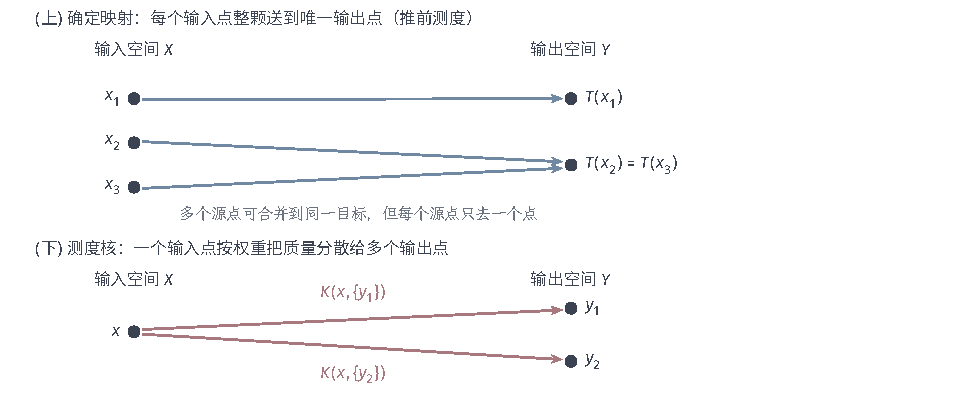
\includegraphics[width=169mm]{figures/00-shared/mathematical-preliminaries-upper/05-space-and-geometry/tikz/pushforward-and-kernel/figure.pdf}
\caption{确定映射（推前测度）与测度核的对照。上排：每个输入点的全部质量沿唯一箭头送到一个输出点，多个输入点可以合并到同一目标（$x_2,x_3$），但单个输入点不能拆开。下排：一般测度核允许同一个输入$x$按权重$K(x,\{y_1\})$、$K(x,\{y_2\})$把质量分给多个输出；归一化核满足这些权重之和为$1$。}
\label{fig:pushforward-and-kernel}
\end{figure*}

\subsubsection{核积分与核复合}

\paragraph{输出测度与观测函数的传递}

有了输入测度$\mu$和核$K$，怎样得到输出空间上的总测度？
直观上是“每个输入$x$送出质量分布$K_x$，再按$\mu$中$x$的权重把这些分布加权求和”：
\[
 (\mu K)(B)=\int_X K(x,B)\,\mu(dx).
\]
对固定$x$，$K(x,\cdot)$可数可加；对不相交的$B_n$，用单调收敛把求和与积分交换，可知$\mu K$仍是测度。
其总质量为
\[
 (\mu K)(Y)=\int_XK(x,Y)\,d\mu\leq M\mu(X).
\]
因此统一质量界保证有限输入测度产生有限输出测度；核归一化时总质量守恒$(\mu K)(Y)=\mu(X)$，一般核则不守恒。

对应地，输出函数$g$沿核传回输入：
\[
 Kg(x)=\int_Y g(y)\,K(x,dy).
\]
对非负可测$g$，$Kg$可测，并且有核积分恒等式
\begin{equation}
 \int_Y g\,d(\mu K)=\int_X Kg\,d\mu,
 \label{eq:measure-kernel-integral}
\end{equation}
即“先核传递再对输出取平均”等于“先沿核算条件平均、再对输入平均”。
有界函数满足$|Kg(x)|\leq M\|g\|_\infty$；一般有符号函数在绝对可积时可选取可测版本后合并。

用一个小数字例子核对。
输入点$a,b$的质量分别为$1,2$，输出点$0,1$；核的两行取$(2,1)$和$(0,2)$（注意这不是归一化核）。
输出两点的质量分别是
\[
 1\cdot2+2\cdot0=2,\qquad 1\cdot1+2\cdot2=5,
\]
总质量$7$等于按输入权重累计的行总质量$1\cdot3+2\cdot2=7$，但不等于输入总质量$3$。
取$g(y)=y$，沿核的条件平均在两行是$1,2$，输入加权$1\cdot1+2\cdot2=5$，与直接对输出积分一致。

\paragraph{连续两次传递的复合}

若$K:X\leadsto Y$、$L:Y\leadsto Z$，从$X$经$Y$到$Z$的总规则是“先按$K_x$在$Y$中取一个中间点，再按该点的$L$核送出”，即
\[
 (KL)(x,C)=\int_Y L(y,C)\,K(x,dy).
\]
统一质量界相乘：$(KL)(x,Z)\leq N\,K(x,Y)\leq NM$；两核都归一化时复合核也归一化。
先后传递与先后传回观测彼此一致：
\[
 (\mu K)L=\mu(KL),\qquad (KL)g=K(Lg).
\]
把$K,L$取成映射$T,S$的点核，就恢复$K_TK_S=K_{S\circ T}$，说明核复合是映射复合的自然推广。

\subsubsection{测度值映射的可测性}

\paragraph{用集合质量检验测度族的可测依赖}

有时要把“一个$X$上的点映到$Y$上的一整项测度”本身看成映射$F:X\to\mathcal M_+(Y)$。
怎样定义这种映射可测？
在测度空间$\mathcal M_+(Y)$上，用所有评价映射
\[
 e_B(\nu)=\nu(B),\qquad B\in\mathcal B
\]
生成一个$\sigma$代数。
在这个结构下，$F$可测当且仅当对每个$B$，$x\mapsto F(x)(B)$都是可测函数——也就是说，\emph{每个目标集合收到的质量随输入可测地变化}。
测度核的第二条条件恰好保证$x\mapsto K_x$是这样一项可测的测度值映射。

一个直接的例子是经验测度：给定非负权重$a_i$，
\[
 F(y_1,\ldots,y_n)=\sum_{i=1}^n a_i\delta_{y_i}
\]
对每个$B$的评价$\sum_i a_i\mathbf 1_B(y_i)$都是坐标的可测函数，所以“由样本点形成加权点测度”这个操作是可测的；取$a_i=1/n$就是常用的\term{经验测度}。

\subsection{联合测度与测度\term{核分解}}

输出测度$\mu K$只告诉我们目标端最终收到多少质量，却丢掉了“哪部分输入送给了哪部分输出”的配对信息。
要保留这种信息，必须在乘积空间$X\times Y$上使用联合测度。
本小节先正向构造联合测度，再研究反向问题：给定一个联合测度，能否恢复“给定输入时输出的条件分布”。

\subsubsection{由输入测度和核构造联合测度}

\paragraph{联合权重、两个边缘与乘积特例}

给定有限输入测度$\mu$和核$K:X\leadsto Y$，先在矩形上规定
\[
 J(A\times B)=\int_A K(x,B)\,\mu(dx),
\]
含义是“从$A$中的输入出发、最终落入$B$的质量”。
再推广到一般乘积可测集：
\[
 J(E)=\int_X\left[\int_Y\mathbf 1_E(x,y)\,K(x,dy)\right]\mu(dx).
\]
截面积分关于$x$可测，单调收敛保证$J$可数可加，总质量不超过$M\mu(X)$。

在矩形上取$B=Y$和$A=X$，得到两个边缘：
\[
 (\pi_X)_\#J(A)=\int_A K(x,Y)\,d\mu(x),\qquad
 (\pi_Y)_\#J=\mu K.
\]
第一边缘是“每个输入实际送出多少质量”，只有核归一化时它才等于原$\mu$；第二边缘就是前面的输出测度。
对联合函数$h$，相应积分规则为
\begin{equation}
 \int_{X\times Y}h\,dJ
 =\int_X\int_Y h(x,y)\,K(x,dy)\,\mu(dx),
 \label{eq:measure-joint-integral}
\end{equation}
记号$\mu(dx)K(x,dy)$表示的就是这种“先输入、再沿条件核”的联合累计。

两个特例帮助定位。
若$K(x,\cdot)=\nu$与$x$无关，$J$就是乘积测度$\mu\otimes\nu$（“输入与输出独立地各算各的”）。
若$K=K_T$是确定映射的点核，$J=(\operatorname{id},T)_\#\mu$是集中在图像$\{(x,Tx)\}$上的\term{图测度}（“输出完全由输入确定”）。
乘积和图测度都只是联合测度的特例；给定同样的边缘，通常还有许多携带不同配对信息的联合测度。

\subsubsection{从联合测度反求测度核}

\paragraph{子$\sigma$代数上的\term{条件积分}与观测值表示}

反向分解的核心问题是：只看输入$x$，输出$y$的条件分布是什么？
为理解它，先看一个预备概念——在较粗的信息下保留积分。
在有限测度空间上，给定可积函数$h$和子$\sigma$代数$\mathcal G$，把$\nu(A)=\int_Ah\,d\mu$限制到$\mathcal G$的集合上。
这个受限赋权对$\mu|_{\mathcal G}$绝对连续，由Radon–Nikodym定理存在$\mathcal G$可测的函数$H$，使
\[
 \int_A H\,d\mu=\int_A h\,d\mu\qquad(A\in\mathcal G).
\]
$H$就是$h$在“只能看到$\mathcal G$”时的积分代表：它保存每个粗集合上的累计，却不必逐点等于$h$。
这正是条件期望/条件积分的思想，这里只用它作为分解的桥梁。

若$\mathcal G=\sigma(S)$由某个观测$S$生成，则$H$只通过$S$取值：$H=\phi\circ S$。
也就是说，只能根据观测$S$得到的信息，必然是观测值的函数，而不能在“$S$相同、但不可区分”的点上给出不同值。

把这一想法用于联合测度$J$：令第一坐标投影为$\pi_X$、$\mathcal G=\sigma(\pi_X)$，对每个目标集$B$取$h=\mathbf 1_B(y)$。
条件积分只依赖$x$，记为$k_B(x)$，则
\[
 \int_A k_B(x)\,d\mu_X(x)=J(A\times B),
\]
其中$\mu_X=(\pi_X)_\#J$是第一边缘。
$k_B(x)$正是“给定输入$x$时输出落入$B$的条件概率”的雏形，取值在$[0,1]$。
但对每个$B$分别找到$k_B$，还不能保证它们彼此拼得起来：对固定的$x$，要求$B\mapsto k_B(x)$可加、且$k_Y(x)=1$；而逐集合用Radon–Nikodym定理得到的代表，可能在不同集合上各自挑了一个零测集上的取值，彼此冲突。
在有限情形里这毫无问题——条件分布就是联合频数表里每一行归一化：行内各列频数除以行和，天然加起来等于$1$。
一般空间的困难只在于“行”可以有不可数个、没有一张写好的频数表，需要下面的存在定理保证能选出一套彼此一致的行分布。

\paragraph{标准Borel范围内的联合分解}

\term{核分解}（条件分布的正则化）在足够规整的可测空间中一定存在。

\begin{theorem}[测度的核分解]
\label{thm:measure-disintegration}
设$X,Y$为标准Borel空间，$J$是$X\times Y$上的非零有限测度，第一边缘$\mu_X=(\pi_X)_\#J$。
则存在归一化测度核$K:X\leadsto Y$，使
\[
 J(A\times B)=\int_A K(x,B)\,\mu_X(dx),
\]
即
\[
 J=\mu_X(dx)\,K(x,dy),
\]
且第二边缘为$\mu_XK$。
\end{theorem}

直觉上，联合测度总能解释成“先按$\mu_X$抽取输入$x$，再按条件核$K_x$抽取输出$y$”；归一化是按实际第一边缘分解的结果，并不要求$J$本身是概率。
标准Borel空间的规整之处，是它的可测集合能由可数个基本集合决定，于是前面逐个集合得到的条件概率可以改造成一套彼此相容的行分布（这叫“正则版本”）；每个$x$送出的那一项$K_x$只在$\mu_X$的一个零集之外唯一——也就是说，对输入中几乎必然取到的点，条件分布没有歧义，个别零测输入点上怎样指定都不影响计算。

对角图测度的例子很能说明“联合密度”和“条件核”的区别。
令$X=Y=[0,1]$，$J=(\operatorname{id},\operatorname{id})_\#\lambda$集中在对角线$\{x=y\}$上。
它的两个边缘都是$\lambda$，但$\lambda\otimes\lambda$给对角线质量$0$、$J$给它质量$1$，所以$J$相对乘积测度没有密度；尽管如此，条件核$K(x,\cdot)=\delta_x$仍然把$J$完整重建。
因此“没有联合密度”和“没有条件分解”是两回事。

\subsection{建立共同空间后的测度比较}

有了推前和核，就能把位于不同空间的测度“搬到同一个地方”再用上一节的指标比较。
本小节强调：比较的对象是变换后的输出，比较结果只反映这种特定表示能看到的差异；表示本身可能丢失信息。

\subsubsection{目标空间与共同表示}

\paragraph{指定映射后的目标端差异}

给定输入空间上的概率$P$、目标空间上的概率$Q$和固定映射$T:X\to Y$，先形成$R=T_\#P$，再在$Y$上比较$R$与$Q$。
我们不能直接对不同空间的$P,Q$做密度相减，因为同一个目标事件$B$对应的其实是源事件$T^{-1}(B)$。
用核时同理，取$R=PK$；一般核可能改变总质量，比较前要先核对输出范围。

各类指标需要的条件照旧：TV、Hellinger只需在$Y$上取共同有限参考$R+Q$；$D_{\mathrm{KL}}(R\|Q)$要检查$R\ll Q$和对数可积性；Wasserstein则要求$(Y,d_Y)$是Polish空间且$R,Q$有有限$p$阶矩。
尤其要注意：输出矩要在输出空间计算，
\[
 \int d_Y(y,y_0)^p\,dR(y)=\int d_Y(Tx,y_0)^p\,dP(x),
\]
源空间的矩不能代替它。
例如输入是$[0,1]$上的均匀分布、$T(x)=1/x$（$x>0$），输入各阶矩都有限，但输出矩$\int_0^1x^{-p}dx=+\infty$，输出分布无法进入Wasserstein的有限距离范围。

\paragraph{在共同表示空间中比较}

若两侧都要换表示，就固定映射$S:X\to Z$、$T:Y\to Z$，在第三个空间$Z$上比较$S_\#P$与$T_\#Q$。
比较什么指标，就在$Z$上配什么结构：比权重差异取共同参考，比几何差异则让$Z$成为Polish度量空间并核对矩，再算$W_p^Z(S_\#P,T_\#Q)$。
$X,Y$内部各自的距离$d_X,d_Y$并不能自动给出一个跨空间距离$d(x,y)$。
这种比较的结果依赖所选表示：若把两侧都映成同一个常值，输出当然完全相同，却只说明该常值表示看不到任何输入差异，不能说明原对象相同。

\subsubsection{输出规则与可辨认范围}

\paragraph{确定映射下的信息丢失}

取$P_1=\delta_{-1}$、$P_2=\delta_1$和绝对值映射$T(x)=|x|$：两个截然不同的输入分布推前后都变成$\delta_1$，目标端TV、Hellinger、Wasserstein差异全部为零。
输出相同只意味着“用$|x|$这个观测分不开$+1$和$-1$”。

对同一个映射$T$，比较在变换后只会变小：逐事件有
\[
 |(T_\#P_1)(B)-(T_\#P_2)(B)|
 =|P_1(T^{-1}B)-P_2(T^{-1}B)|
 \leq\operatorname{TV}(P_1,P_2),
\]
取上确界得
\[
 \operatorname{TV}(T_\#P_1,T_\#P_2)\leq\operatorname{TV}(P_1,P_2).
\]
原因是输出端能检验的事件，只对应输入端的一部分事件（原像）。
但两侧用的是\emph{不同}表示时，这个收缩不成立：同为$\delta_0$的输入，经$S(0)=0$和$T(0)=1)$后输出TV为$1$。

\paragraph{同一归一化测度核下的TV控制}

固定同一个归一化核$K$，输出差为
\[
 |(PK)(B)-(QK)(B)|
 =\left|\int_XK(x,B)\,d(P-Q)(x)\right|.
\]
由于$0\leq K(x,B)\leq1$，利用TV的$[0,1]$测试表示，每个事件差不超过$\operatorname{TV}(P,Q)$，故
\[
 \operatorname{TV}(PK,QK)\leq\operatorname{TV}(P,Q).
\]
同一个随机通道不会增大可区分性，这就是“数据处理”在TV下的形式。
条件是同一核且归一化：核不同、或核不归一化（总质量改变）时结论不适用。

\paragraph{共同输入构造耦合上界}

若两个输出来自同一个带随机性的源，可用一个共同空间上的映射$F,G$构造它们的耦合$\gamma=(F,G)_\#R$，其两边缘为$F_\#R,G_\#R$。
当两输出在同一Polish空间且矩有限时，
\[
 W_p^p(F_\#R,G_\#R)
 \leq\int d(F(\omega),G(\omega))^p\,dR(\omega).
\]
应用中共同源可以是“共享噪声”：用同一个随机种子驱动两个随机系统，输出差异可用输入空间中$F,G$的距离上界控制。
这只给出一个可行耦合的成本上界，不一定最优。

\subsection{给定跨空间成本的运输比较}

到目前为止，比较要么发生在同一空间，要么先经表示映到同一空间。
但有时源空间$X$和目标空间$Y$天然不同，我们想直接问：把$X$上的质量改造成$Y$上的质量，最少要付出多大代价？
这时必须由问题本身给定一份跨空间成本表，数学不会自动从两个内部距离造出它。

\subsubsection{乘积空间上的耦合与成本}

\paragraph{跨空间质量匹配与成本累计}

把耦合推广到$X\times Y$：$\Pi(P,Q)$是所有满足
\[
 \gamma(A\times Y)=P(A),\qquad \gamma(X\times B)=Q(B)
\]
的跨空间联合概率，两个边缘约束分别保证“源质量不增不减”和“目标收到恰好的量”。
再给定一个非负的、对乘积可测的成本函数$c:X\times Y\to[0,\infty]$，定义最优运输成本
\[
 \mathcal C_c(P,Q)
 =\inf_{\gamma\in\Pi(P,Q)}\int c(x,y)\,d\gamma(x,y).
\]
它在所有质量守恒的配对中找总代价最小的一个。

请注意$\mathcal C_c$一般不是距离：成本$c$未必对称，甚至两侧空间不同时无从谈对称；取$c\equiv0$会让任何$P,Q$的成本都是零。
只有当$X=Y$、取$c(x,y)=d(x,y)^p$且矩有限时，它才成为$W_p^p$。

\subsubsection{运输映射与\term{运输计划}}

\paragraph{不可拆分的映射与可拆分的计划}

历史上有两个版本的运输问题。
\term{Monge问题}要求每个源点的质量完整送到一个目标点，即在约束$T_\#P=Q$下最小化$\int c(x,T(x))\,dP$。
\term{Kantorovich问题}放松为允许拆分：在全部耦合$\gamma\in\Pi(P,Q)$中最小化$\int c\,d\gamma$。
在标准Borel空间，计划还可由核分解写成$P(dx)K(x,dy)$，其中$K$由第一边缘$P$分解故归一化，约束$PK=Q$表示每个源点送出的总质量为$1$、各目标收到的总量正确。

一个最小的例子说明放松拆分为什么必要。
源只有一个点$X=\{0\}$，目标有两个点$Y=\{-1,1\}$，$P=\delta_0$而$Q=\frac12\delta_{-1}+\frac12\delta_1$。
任何确定映射只能把唯一源点送到一个目标，Monge问题无解；但计划
\[
 \gamma=\tfrac12\delta_{(0,-1)}+\tfrac12\delta_{(0,1)}
\]
允许把源点的质量对半拆，满足全部约束。
反过来，任何可行映射$T$的图计划都是一个Kantorovich耦合，所以映射问题嵌入计划问题；计划可行不代表映射可行。

\subsubsection{成本判定与比较范围}

\paragraph{可行、有限与达到分别判断}

使用最优运输成本时要分三步检查，不能混为一谈。
第一，可行性：独立耦合$P\otimes Q$总在$\Pi(P,Q)$中，所以计划可行域非空（这与Monge问题可能无解形成对照）。
第二，有限性：要有至少一个有限成本的候选，例如$\int c\,d(P\otimes Q)<\infty$；若$c$处处为$+\infty$，最优值只能是无穷。
第三，达到性：最小值是否真的被某个耦合取到，还需紧性与成本的下半连续性；其证明要用到\ref{sec:measure-tightness}小节的一致紧性和下半连续积分界，这里先引用结论。

\paragraph{目标匹配、运输代价与结构比较边界}

最后用一个小例子把两类问题彻底分开。
取$X=\{a\}$、$Y=\{b\}$、$P=\delta_a$、$Q=\delta_b$、$T(a)=b$，并规定$c(a,b)=7$。
在输出端，$T_\#P=Q$，匹配得完美无缺，同空间差异为$0$；但实现这个匹配的唯一跨空间运输成本是$7$。
“是否得到了目标分布”和“得到它要花多大代价”显然是两个问题。
因此跨空间比较之前必须先明确给定的是映射、核、共同表示还是成本函数；仅凭两个空间各自的内部距离，本书并不推导空间之间的“内在结构距离”，那是更专门的理论。

\section{测度的收敛与极限操作}
\label{sec:measure-convergence}

有了比较两个概率分布的各种指标，自然要问：一整列分布$P_1,P_2,\ldots$什么时候算趋近于某个$P$？
这个问题没有唯一答案，因为“趋近”取决于我们用什么探针去观测。
本节按探针从强到弱排列几种收敛：要求每个事件的误差一致消失的全变差收敛、只要求有界连续观测收敛的弱收敛、再加上距离矩尾部控制的Wasserstein收敛。
然后建立弱收敛下三件常用的事——事件概率怎么读、连续变换是否保持收敛、无界成本的极限下界——并回答“一族分布是否总能挑出收敛子列”。
最后把序列换成随时间变化的测度曲线，提醒不同时间尺度上的极限不能混用。
本节的比较都在同一个固定空间进行；不同空间的对象要先按上一节映到共同空间。

\subsection{测度序列的收敛方式}
\label{sec:measure-sequence-convergence}

\subsubsection{\term{逐集收敛}与全变差收敛}

\paragraph{从比较误差定义趋近}

最强的常用要求是全变差收敛：
\[
 \operatorname{TV}(P_n,P)\to0.
\]
它的含义是：存在一个与事件无关的误差界（就是TV）趋于零，从而\emph{同时}控制所有可测事件。
由前面的不等式，TV收敛等价于Hellinger收敛；KL收敛通过Pinsker界足以推出TV收敛，但反过来不成立（回想$P_\varepsilon=(1-\varepsilon)\delta_0+\varepsilon\delta_1$与$\delta_0$）。

把要求放松一档得到逐集收敛：对每一个\emph{固定}的事件$A$，
\[
 P_n(A)\to P(A).
\]
两者的差别完全在量词上。逐集收敛时，给定精度后需要等多少项$N$可以随事件$A$而变——复杂事件可能要等很久；TV收敛则要求同一个$N$对所有事件一起生效。
因此TV收敛必然推出逐集收敛，反之不然。
不过逐集收敛已经足以控制任意固定的有界可测函数$g$：先用简单函数在$\|g\|_\infty$意义下一致逼近$g$，再利用概率总质量为$1$控制逼近误差，得到
\[
 \int g\,dP_n\to\int g\,dP.
\]

\subsubsection{\term{弱收敛}与连续测试}

\paragraph{弱收敛与位置移动}

再放松一档，连“每个事件”都不要求，只保留对连续观测量的控制。
称$P_n$弱收敛到$P$，记作$P_n\Rightarrow P$，若对每个有界连续函数$\varphi$都有
\[
 \int\varphi\,dP_n\to\int\varphi\,dP.
\]
为什么只用连续函数做探针？因为事件指示函数$\mathbf 1_A$在集合边界上通常是跳变的，分布质量在边界附近的微小挪动会让$P_n(A)$剧烈变化，却不会明显影响任何连续函数的平均。

标准例子正是“质量在位置上不断靠近”。
取
\[
 P_n=\delta_{1/n},\qquad P=\delta_0.
\]
对任意有界连续$\varphi$，积分就是函数值$\varphi(1/n)\to\varphi(0)$，所以$P_n\Rightarrow P$；但事件$\{0\}$的概率始终是$0$而不是$1$，TV距离也始终为$1$。
质量明明在几何上越来越接近，逐事件比较却认为毫无进展——这清楚说明收敛结论依赖于所选标准。

\subsubsection{Wasserstein收敛与矩条件}

\paragraph{弱趋近与距离尾部的共同控制}

弱收敛只管“局部、有界”的观测，不管远处的质量；\term{Wasserstein距离}则会为远距离移动付费。
在Polish空间上，对$P_n,P\in\mathcal P_p(X)$有标准判据
\begin{equation}
 W_p(P_n,P)\to0
 \quad\Longleftrightarrow\quad
 P_n\Rightarrow P
 \ \text{且}\
 \int d(x,x_0)^p\,dP_n\to\int d(x,x_0)^p\,dP.
 \label{eq:measure-wasserstein-criterion}
\end{equation}
——既要在所有有界连续探针上收敛，又要$p$阶矩收敛。
矩条件控制的是“远处的小质量”。
记$z(x)=d(x,x_0)^p$。
先只用弱收敛，把它截断成有界函数$\min(z,R)$，能推出积分在近处（离基点不超过$R$）收敛；真正的差别在截断之外的“尾部”$\int(z-R)_+\,dP_n$。
全矩收敛加上弱收敛，可以推出一个对所有$n$统一成立的尾部估计：先取一个足够大的$R$把\emph{极限测度}的尾部压到很小，再用弱收敛保证$n$足够大时$P_n$在“$R$以外”的概率也很小，两者合起来就把整列的尾部一起压住。
这正是“距离的$p$次方关于这列测度一致可积”的含义；仅有“每个$P_n$自己的矩有限”给不出这种一致性。

\paragraph{小概率远距离的反例}

“每项矩有限”为什么不够？看下面的序列：
\[
 P_n=(1-n^{-p})\delta_0+n^{-p}\delta_n,\qquad P=\delta_0.
\]
远端那一点的概率只有$n^{-p}$，对任意有界连续观测的贡献趋于零，故$P_n\Rightarrow P$；每一项的$p$阶矩也都有限。
但把远端质量搬回原点要走距离$n$，代价是
\[
 W_p(P_n,P)^p=n^{-p}\cdot n^p=1,
\]
永不趋于零。
这把两件事分得很清楚：远端质量的\emph{概率}可以很小，但乘上很大的\emph{距离}后总代价仍是常数；没有对尾部的共同控制，Wasserstein不会收敛。

\begin{figure*}[htbp]
\centering
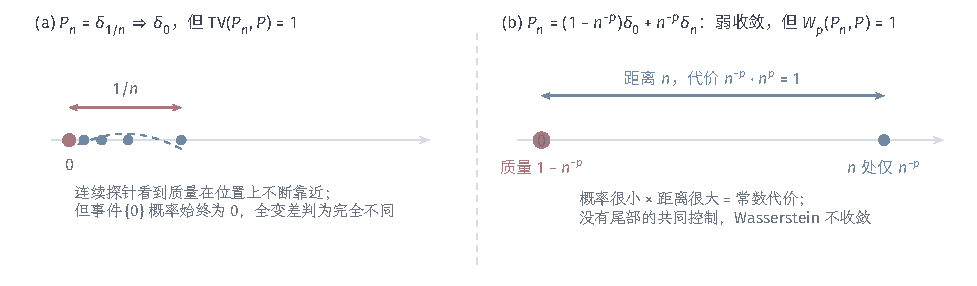
\includegraphics[width=169mm]{figures/00-shared/mathematical-preliminaries-upper/05-space-and-geometry/tikz/convergence-modes/figure.pdf}
\caption{两种“看起来在靠近、却不按更强标准收敛”的典型情形。(a) $P_n=\delta_{1/n}$在几何上不断靠近$\delta_0$，连续探针读数$\varphi(1/n)\to\varphi(0)$，故弱收敛；但事件$\{0\}$的概率始终为$0$，全变差距离恒为$1$。(b) $P_n=(1-n^{-p})\delta_0+n^{-p}\delta_n$弱收敛、每项矩都有限，但把$n$处那一点概率$n^{-p}$搬回原点的$p$次代价$n^{-p}\cdot n^p=1$，故$W_p$不趋于零。}
\label{fig:convergence-modes}
\end{figure*}

\subsection{弱收敛的判据与稳定性}

弱收敛只直接定义在有界连续测试上，实际使用时还想知道：事件概率能不能读、经过映射后还收不收敛、无界成本的极限保不保住下界。
这三者都是弱收敛这同一个概念下的推论，不是新的收敛方式。

\subsubsection{事件概率与边界质量}

弱收敛只在连续函数的积分上成立，可实际问题里我们常想直接读“落在某集合里的概率”。
什么时候这件事合法？答案是：只要极限分布不在该集合的\emph{边界}上放质量。
下面的\term{Portmanteau定理}先给出用开集、闭集表述的形式，事件概率的读法是它的直接推论：
\[
 P_n\Rightarrow P
\]
等价于对所有闭集$C$有$\limsup_nP_n(C)\leq P(C)$，也等价于对所有开集$G$有$\liminf_nP_n(G)\geq P(G)$。
用一句话说就是：当质量整体向$P$靠拢时，落在一个闭集里的概率最终不会超过$P$给它的概率（边界附近的质量可以溜出去），落在一个开集里的概率最终不会少于$P$给它的概率（质量可以从边界溜进来）。
它的实用推论是：如果极限测度不给集合$A$的边界质量，即$P(\partial A)=0$，那么
\[
 P_n(A)\to P(A).
\]

闭集方向可以直观地证明。对闭集$C$，用连续函数
\[
 h_k(x)=\max\{1-k\,d(x,C),0\}
\]
从外面“软包”一层：$h_k$有界连续、在$C$上等于$1$、离开$C$超过$1/k$就降到$0$，且$h_k\downarrow\mathbf 1_C$。
由$\mathbf 1_C\leq h_k$和弱收敛，
\[
 \limsup_nP_n(C)\leq\int h_k\,dP;
\]
再令$k\to\infty$，由支配收敛得到$\limsup_nP_n(C)\leq P(C)$。
开集方向取补集即可。
一般集合用内部$A^\circ$和闭包$\overline A$夹住：
\[
 P(A^\circ)\leq\liminf_nP_n(A)\leq\limsup_nP_n(A)\leq P(\overline A),
\]
只有边界质量为零时两端才相等。
回看$\delta_{1/n}$与事件$\{0\}$：极限测度恰好把质量放在边界$\{0\}$上，条件失败，所以$P_n(\{0\})$不收敛到$P(\{0\})$。
问题的根源始终是探针在集合边界上的跳变。

\subsubsection{连续推前与边缘保持}

弱收敛在连续变换下保持。
设$T:X\to Y$连续且$P_n\Rightarrow P$，对目标端任意有界连续$\varphi$，
\[
 \int\varphi\,d(T_\#P_n)=\int\varphi\circ T\,dP_n\to\int\varphi\circ T\,dP,
\]
因为$\varphi\circ T$仍有界连续。故
\[
 T_\#P_n\Rightarrow T_\#P.
\]
注意结论依赖\emph{连续性}：若$T$只可测不连续，可能失败。例如$P_n=\delta_{1/n}$、$P=\delta_0$，取$T=\mathbf 1_{\{0\}}$，则$T_\#P_n=\delta_0$而$T_\#P=\delta_1$。
连续坐标投影是这一结论的重要应用：若耦合列弱收敛，其两个边缘也分别弱收敛到极限耦合的边缘——这正是后面最优运输计划取极限时仍满足边缘约束的依据。

\subsubsection{\term{下半连续}成本的极限下界}

运输成本通常无界，不能直接当弱收敛的测试，但在下半连续时能保住一个方向的不等式。
所谓\term{下半连续}，直观上就是“极限点处的值不会突然变贵”：当$x_n\to x$时，恒有$c(x)\leq\liminf_n c(x_n)$——成本函数允许在某点向上跳变（如$c(x)=0$只在原点、其余为$1$），但不允许向下塌。
在这个条件下，非负下半连续函数$c$可以用一列有界连续函数从下方逼近：
\[
 c_k(x)=\min\left\{k,\ \inf_y[c(y)+k\,d(x,y)]\right\},
\]
$c_k$的$k$-Lipschitz连续性可直接验证，$c_k\uparrow c$则由下半连续性保证（若某点严格小于$c(x)$，近似取到的点必趋向$x$，与下半连续矛盾）。

设$P_n\Rightarrow P$。先固定$k$用弱收敛，再令$k\to\infty$用单调收敛：
\[
 \int c\,dP=\lim_k\int c_k\,dP
 =\lim_k\lim_n\int c_k\,dP_n
 \leq\liminf_n\int c\,dP_n.
\]
于是
\begin{equation}
 \int c\,dP\leq\liminf_n\int c\,dP_n.
 \label{eq:measure-lsc-portmanteau}
\end{equation}
直觉是：下半连续函数在“极限点处的值不超过附近点的下极限”，积分把这个性质继承下来；极限分布处的最优成本不会比逼近序列的成本下极限更贵。
这里测度本身在变，不能直接套用固定测度的Fatou引理。
这条不等式与紧性配合，正好证明最优运输计划可以取到。

\subsection{\term{一致紧性}与弱子列}
\label{sec:measure-tightness}

前面都是“先有候选极限$P$，再判断$P_n$是否趋近它”。
反过来的问题是：不给定极限，一列概率是否至少能挑出一个收敛子列？
在实轴上有界序列靠紧性总能取子列；一般空间中，类似结论成立的关键是“质量不能跑到任何紧集之外”。

\paragraph{一致紧性与极限子列}

称概率族$\mathcal F$一致紧，若对每个$\varepsilon>0$都能找到\emph{同一个}紧集$K_\varepsilon$，使族中每一个$P$都满足
\[
 P(X\setminus K_\varepsilon)<\varepsilon.
\]
紧集可以随精度$\varepsilon$变，但不能随具体的$P$变——要求的是“一整个族共用一个紧笼子”。
在一般度量空间中“有界”不一定“紧”，所以统一的矩界不能无条件代替一致紧性。

\begin{theorem}[\term{Prokhorov定理}，子列形式]
\label{thm:measure-prokhorov}
在Polish空间上，概率族$\mathcal F$一致紧，当且仅当$\mathcal F$中任意序列都有弱收敛到某个Borel概率的子列。
\end{theorem}

极限概率不必属于原来的族；“某种收敛如何定义”和“是否保证存在收敛子列”是两个独立判断。
质量逃逸的典型反例是$\{\delta_n:n\geq1\}$：每个$\delta_n$本身都是紧支撑的，但不存在一个能同时留住所有$n$的紧集，序列没有弱收敛到概率的子列。

\paragraph{固定边缘下的最优计划}

现在把紧性和下半连续界用到最优运输上，补齐“最优计划存在”的证明三步。
先证明\emph{整个}耦合族$\Pi(P,Q)$一致紧，而不只是某个耦合紧。
给定$\varepsilon>0$，用紧集$K,L$分别把$P,Q$的大部分质量套住：
\[
 P(K^c)<\frac\varepsilon2,\qquad Q(L^c)<\frac\varepsilon2.
\]
对任意$\gamma\in\Pi(P,Q)$，由边缘约束，
\[
 \gamma((K\times L)^c)\leq\gamma(K^c\times Y)+\gamma(X\times L^c)
 =P(K^c)+Q(L^c)<\varepsilon.
\]
于是所有耦合共用同一个紧集$K\times L$。

设成本$c$非负下半连续且至少有一个有限成本耦合，最优值
\[
 I=\inf_{\gamma\in\Pi(P,Q)}\int c\,d\gamma<\infty.
\]
取一列成本趋于$I$的耦合$\gamma_n$；由一致紧性和Prokhorov定理抽出弱收敛子列$\gamma_{n_k}\Rightarrow\gamma$。
连续投影保持边缘，所以$\gamma$仍是$P,Q$的耦合；下半连续积分界给出
\[
 \int c\,d\gamma\leq\liminf_k\int c\,d\gamma_{n_k}=I,
\]
而$\gamma$可行又给出反向不等式，故最小值在$\gamma$处达到。
这就把“紧子列—边缘保持—成本下界”三步接齐。
结论只保证最优\emph{计划}存在，不保证最优\emph{映射}存在；成本也必须下半连续。

\subsection{测度曲线与参数极限}

\paragraph{由序列判据读取时间连续性}

把序号$n$换成连续时间$t$，就得到概率曲线$t\mapsto\mu_t$。
称它弱连续，若每个有界连续探针的读数关于$t$连续，即
\[
 t_n\to t\ \Longrightarrow\ \mu_{t_n}\Rightarrow\mu_t.
\]
若各时刻都在$\mathcal P_p(X)$中，还可要求$W_p(\mu_{t_n},\mu_t)\to0$，由矩判据~\eqref{eq:measure-wasserstein-criterion}，这额外控制了尾部。

点质量曲线$\mu_t=\delta_t$再次显示标准的作用：
\[
 W_p(\mu_s,\mu_t)=|s-t|,
\]
所以它关于$W_p$连续；但$s\neq t$时TV恒为$1$，在全变差意义下处处不连续。
若不同时刻的测度位于不同空间，还要先固定到一个共同空间的表示，才能谈连续性。

\paragraph{固定时刻、有限时域与长时间}

比较一条近似曲线$\mu_t^h$与目标曲线$\mu_t$时，要区分三种越来越强的说法，它们的量词不能互换：
\begin{enumerate}
 \item \emph{固定时刻}：对每个固定$t$，$W_p(\mu_t^h,\mu_t)\to0$；
 \item \emph{有限时域一致}：对每个固定$T$，$\sup_{0\leq t\leq T}W_p(\mu_t^h,\mu_t)\to0$；
 \item \emph{长时间极限}：$t\to\infty$时曲线本身是否趋于某个极限。
\end{enumerate}
取$\mu_t=\delta_0$、$\mu_t^h=\delta_{ht}$（$h>0$）：固定$t$时误差为$ht\to0$，有限区间$[0,T]$上最大误差为$hT\to0$，但在随$h$移动的时刻$t=1/h$误差恒为$1$，所以在$t\geq0$全域上不一致收敛。
这提醒我们：数值近似在每个固定时刻、每个有限时间区间上可靠，并不自动推出长时间结论；演化方程、数值稳定性和极限交换都留给后续问题专门处理。


\FloatBarrier
\section{本章小结}

本章把微积分中“沿长度、体积累计”的想法推广到任意对象组成的空间，得到五条相互衔接的认识。

第一，测量分两层，而且两层互不相同。$\sigma$代数规定\emph{哪些集合看得见}，测度规定\emph{看得见的集合有多大}；还要把测度与度量分清：测度吃进一个集合给出份量，度量吃进两个点给出距离，同一底集上两者各自独立选择，讨论Wasserstein等几何问题时才在测度之外另加度量。同一个可测范围上可以配任意多种权重，也可以通过子$\sigma$代数在不删点的情况下降低分辨能力。有限、概率、$\sigma$有限是三种强度不同的质量条件，零测集和完备化说明哪些点上的例外可以忽略。当开集参与进来时，Borel结构、Polish空间和支持把“测量”与“位置”联系起来，而一般积分、三条收敛定理、乘积测度与Tonelli/Fubini都在明确条件下原样沿用。

第二，同一空间上的测度比较从零集关系开始，再到表示和定量指标。绝对连续、等价和相互奇异刻画零集之间的包含、重合与分离；Radon–Nikodym密度是两种称重方式的局部换算比例，Lebesgue分解把能这样换算的部分和集中在零集上的部分分开。为描述测度之差引入了有符号测度及其Jordan分解与总变差。全变差、Hellinger和KL只比较同一位置上的事件或密度，Wasserstein还要计入两点间的距离；积分概率度量把它们统一成“某类探针上的最大读数差”。这些指标回答的问题不同，不存在一个能代替其余的“万能距离”。

第三，跨空间时质量的传递规则从确定走向随机。可测映射的推前回答“每个输出事件收到多少输入质量”，输出积分等于输入上的复合积分；测度核把“一个输入对应一个点”放宽为“一个输入对应一项目标测度”，核积分和核复合分别统一了输出传递与观测传递。联合测度保留输入输出的配对，乘积和确定图是其特例；在标准Borel空间上，联合测度可以沿第一边缘分解为归一化条件核。条件积分只保存粗信息下的累计，条件期望等概率法则在后文展开。

第四，跨空间比较前必须先固定对应关系。给定映射或核以后，比较的是变换后的输出而不是原对象；表示可能丢失信息，所以输出相同不能反推输入相同，不同表示之间也没有收缩性质。给定跨空间成本时，Kantorovich计划允许拆分质量、Monge映射不允许，二者可行域不同；可行、有限、最优值达到要分别靠耦合非空、有限成本候选和紧性加下半连续性来保证。输出匹配为零与运输代价非零可以同时成立。

第五，测度序列是否趋近取决于探针。全变差统一控制所有事件，弱收敛只看有界连续函数，Wasserstein还要加上距离矩的尾部控制；弱收敛通过Portmanteau界读取边界零质量事件，在连续映射下保持，在下半连续成本下只给积分下界。一致紧性经Prokhorov定理保证弱子列，并支撑最优运输计划的存在性；固定时刻、有限时域一致和长时间极限是三种不能互换的逼近。
这些通用操作为后文的随机过程、条件模型、经验测度和策略分析提供了语言，但相应的概率性质、统计保证和生成机制仍需各自的条件。


